%==========================================================
%-------------------- BEGIN PREAMBLE ----------------------
%==========================================================
%\documentclass[12pt]{scrbook}
%\documentclass[12pt, twoside=true]{scrbook} % sidetall nede
%\documentclass[12pt, openany]{book} % brukt

\documentclass[12pt, oneside]{book}

%\documentclass[12pt, twoside]{book}


%\setkomafont{disposition}{\normalfont\bfseries}
\usepackage{Setup/style}
\usepackage{siunitx}
%---------------- custom style -----------------------
%----- equation numbering -------
\numberwithin{equation}{section}     % number within section
%\numberwithin{equation}{subsection} % number within subsection

%----- fig & table numbering -----
\counterwithin{figure}{section}
\counterwithin{table}{section}

%--------- format abstract ---------
\makeatletter
\renewenvironment{abstract}{
    \if@twocolumn
      \section*{\abstractname}
    \else
      \begin{center}
        {\bfseries \large\abstractname\vspace{\z@}}
      \end{center}
      \quotation
    \fi}
    {\if@twocolumn\else\endquotation\fi}
\makeatother

%----------------- tikz ---------------------------
% Define block styles
\tikzstyle{startstop} = [rectangle, rounded corners,
    minimum width=3cm, minimum height=1cm,text centered, draw=black, fill=red!30]
\tikzstyle{io} = [trapezium, trapezium left angle=70, 
    trapezium right angle=110, minimum width=3cm, minimum height=1cm, text centered, text width=3cm, draw=black, fill=blue!30]
\tikzstyle{process} = [rectangle, minimum width=3cm,
    minimum height=1cm, text centered, text width=3cm, 
    draw=black, fill=orange!30] 
\tikzstyle{decision} = [diamond, minimum width=3cm, 
    minimum height=1cm, text centered,text width=2cm, 
    draw=black, fill=green!30]
\tikzstyle{arrow} = [thick,->,>=stealth]
\tikzstyle{block} = [rectangle, draw, fill=blue!20, 
    text width=5em, text centered, rounded corners, minimum height=4em]
\tikzstyle{line} = [draw, -latex']
\tikzstyle{cloud} = [draw, ellipse,fill=red!20, node distance=3cm,
    minimum height=2em]


%---------- insert custom LaTeX commands ----------
\newcommand*{\QED}{\hfill\ensuremath{\square}}
\newcommand{\E}{\mathrm{E}}
\newcommand{\R}{\mathbb{R}}
\newcommand{\X}{\mathbf{X}}
\newcommand{\y}{\mathbf{y}}
\newcommand{\rss}{\mathrm{RSS}}
\newcommand{\MSE}{\mathrm{MSE}}
\newcommand{\Err}{\mathrm{Err}}
\newcommand{\err}{\mathrm{err}}
\newcommand{\bias}{\mathrm{Bias}}
\newcommand{\Var}{\mathrm{Var}}
\DeclareMathOperator*{\argmax}{arg\,max}
\DeclareMathOperator*{\argmin}{arg\,min}
\DeclareMathOperator*{\cv}{CV}
\DeclareMathOperator*{\df}{df}
\newcommand{\T}{\mathcal{T}}

\NewDocumentCommand{\cw}{v}{%
\textbf{\texttt{\textcolor{Blue}{#1}}}%
}


\addbibresource{bibliography.bib}   % Bibliography

% Set graphics path
\graphicspath{{latex/figures/}}

%\usepackage[titles]{tocloft}   % fix spacing in \listoffigures
%\cftsetindents{figure}{0em}{3.5em}

\usepackage[T1]{fontenc}
\usepackage[newcentury]{quotchap}
\usepackage{blindtext}

\usepackage[nouppercase]{scrlayer-scrpage} % header no upper case
\pagestyle{scrheadings}

% no page numbering on begin part and chapter pages 
\usepackage{etoolbox}
\patchcmd{\part}{plain}{empty}{}{}
\patchcmd{\chapter}{plain}{empty}{}{}


\usepackage{biblatex}
\addbibresource{bibliography.bib}
\raggedbottom

%==========================================================
%-------------------- END PREAMBLE ------------------------
%==========================================================



%==========================================================
%-------------------- MAIN CONTENT ------------------------
%==========================================================
\begin{document}

%==========================================================
%------------------------ preface -------------------------
%==========================================================

%------------------ front page -----------------------
\title{
    \Large \textbf{Likelihood-Free Inference Methods for Parameter Identification in Neuroscientific Models}
    \\[8 pt]
    \large by
    \\ [8 pt]
    \large Nicolai Haug
    \\ [40 pt]
    \large \textbf{Thesis}
    \\ [8 pt]
    \large for the degree of
    \\ [8 pt]
    \large \textbf{Master of Science}
    \\ [30 pt]
    
\includegraphics[scale=0.9]{latex/latex-report/3_Images/Logo/UiO/UiO_Segl_300dpi.png}
    %\includegraphics[scale=0.9]{Setup/DUO_UiO_segl.png}
    \\ [30 pt]
    \large Department of Informatics
    \\ [8 pt]
    \large Faculty of Mathematics and Natural Sciences
    \\ [8 pt]
    \large University of Oslo
    \\ [15 pt]
    \large November 2021
}%title end

\author{\vspace{-5ex}}
\date{\vspace{-5ex}}

% ... in Neuronal Models 
% ... in Neuroscientific Models
% ... in Mechanistic Models
% ... in Neuron Models
% ... in Neurological Models 
% ... in Mechanistic Models in Neuroscience
% ... in Neuronal Network Models
% ... in Single Neuron and Neural Network Models
% ... in Single and Network Neuronal Models

\maketitle
\pagenumbering{gobble}

%------------------ first page -----------------------
\textit{} 
\\ [100 pt]
This master's thesis is submitted under the master's program \textit{Computational Science}, with program option \textit{Imaging and Biomedical Computing}, at the Department of Informatics, University of Oslo. The scope of the thesis is 60 credits.
\\ [350 pt]
\textbf{\faCopyright \, Nicolai Haug, 2021}

\href{https://www.duo.uio.no/}{www.duo.uio.no}

Print production: Reprosentralen, University of Oslo
\pagenumbering{gobble}
\clearpage 

%------------------ abstract -------------------------
\frontmatter      % Folios in Roman numerals
%================================================================
%------------------------- Abstract -----------------------------
%================================================================
\chapter*{Abstract}
\addcontentsline{toc}{chapter}{Abstract}
\thispagestyle{plain}

%Limit the abstract to as few words as possible. The abstract should always be less than one page long, and less than 400 words. Be aware that many online referencing systems only allow the first 200 words to be included. No figures or references should be presented.Avoid extensive technical and method details where possible. Should be readable to a literate science reader familiar with your general area, but not necessarily experts-only material. 


A central challenge in building a mechanistic model of neural dynamics is to identify the model parameters consistent with experimental data. Due to intractable likelihoods, traditional methods in the toolkit of statistical inference are inaccessible for many mechanistic models. To overcome intractable likelihoods, simulation-based inference provides a framework for performing rigorous Bayesian inference without requiring numerical evaluation of likelihoods by using only forward simulations. The objective of this thesis is to investigate the viability of simulation-based inference, in particular approximate Bayesian computation (ABC) algorithms, for identifying parameters in mechanistic models of neural dynamics. Specifically, we use rejection ABC (REJ-ABC) and Markov chain Monte Carlo ABC (MCMC-ABC) to infer the conductance parameters in the Hodgkin-Huxley model for initiation and propagation of action potentials and the synaptic weight parameters in the Brunel network model for activity dynamics in local cortical networks. 

It also has the
advantage of returning an entire posterior distribution on the
value of the parameters, rather than a simple point estimate

implement the generic Python library pyLFI 

We implemented REJ-ABC with quantile-based rejection

We extensively varied hyperparameters, and found that

As the curse of dimensionality forces ABC to require a compression of data into low-level summary statistics, we use expert-crafted statistics of spiking activity. 



While rejection ABC (REJ-ABC) uses the prior as a proposal distribution, the efficiency can be improved by using sequentially refined proposal distributions (SMC) (can be said about MCMC also?). We implemented REJ-ABC with quantile-based rejection. 
We extensively varied hyperparameters. We investigated linear regression adjustment (Blum and François, 2010) and the summary statistics approach
by Prangle et al. (2014). [SBI Benchmark]



Because of the curse of dimensionality, ABC requires a compression of the data into low-dimensional summary statistics. We use various summary statistics of neural data obtained from domain knowledge.  expert-crafted summary statistics of spiking activity. If powerful low-dimensional summary statistics are established, traditional techniques can still offer a reasonable performance.

MCMC ABC, which improves the sample efficiency compared to Rej ABC by being guided by a proposal distribution ... MCMC ABC has improved sample efficiency 



In this thesis, we have used ABC with rejection sampling (Rejection ABC) and

In this thesis we implement the generic Python library pyLFI which uses ABC with both rejection and Markov chain Monte Carlo (MCMC) sampling for parameter inference/identification. In particular, we infer the conductance parameters in the Hodgkin-Huxley model for initiation and propagation of action potentials and the synaptic weight parameters in the Brunel network model for activity dynamics in local cortical networks. 

In this thesis, we have used (rejection) ABC (rejection sampling) and (MCMC) ABC (importance sampling) for identifying the conductance parameters in the Hodgkin-Huxley model for initiation and propagation of action potentials and the synaptic weight parameters in the Brunel network model for activity dynamics in local cortical networks. 

The Hodgkin-Huxley formalism is used as basis for many biophysically detailed cell models ...

Many cell models are built on the Hodgkin-Huxley formalism ... so being able to accurately constrain model parameters

using Markov chain Monte Carlo (MCMC) sampling

We were able to accurately constrain the conductance parameters of the Hodgkin-Huxley model as we obtained narrow posteriors with the ground truth parameters in regions of high posterior density. A 
For the Hodgkin-Huxley model we obtain narrow posteriors with the true parameters in regions of high posterior density, indicating that ABC is a viable method for parameter identification in the many cell models built on the Hodgkin formalism. 

As we only investigated models with few parameters, the viability of ABC on high-dimensional problems is yet to explore. 
\newpage 

%--------------- acknowledgements --------------------
%---------------------------------------------------------------
\chapter*{Acknowledgements}
\addcontentsline{toc}{chapter}{Acknowledgements}
\thispagestyle{plain}
%---------------------------------------------------------------

The work in this thesis was conducted at the Centre for Integrative Neuroplasticity (CINPLA).

%Without some people, this thesis would not have been possible. I first want to express my gratitude towards my supervisors professor Gaute Einevoll, associate professor Joakim Sundnes and researcher Alexander Stasik. Thank you all for your great support, guidance and meaningful discussions. I have learned a lot about scientific processes and in great part thanks to you. Thank you Gaute for showing me the world of computational neuroscience.

% AT, for helping with the formalities
% JS, code reviews
% AS, expertise in the field has been invaluable
% GE, keeping the project focused and help with uncovering the fascinating aspects of the neuroscience behind it all

%Working from home during the Covid-19 outbreak has been a challenging experience, but I believe it in some ways has taught me a lot about discipline and communication. 

I would like to thank my friends and family, especially my parents for their unconditional support and love in my years as a student in physics and computational science. I would also like to express my gratitude towards my partner Oda for her endless support throughout my degree. 
\\ [8 pt]

\begin{flushright}

\includegraphics[height = 1.5ex]{latex/latex-report/3_Images/Logo/UiO/uio-colon.pdf}\, \textbf{Nicolai Haug}
\\
Oslo, November 2021
\end{flushright}

\newpage

%----------------- abbreviations ---------------------
%----------------------------------------------------------------
\chapter*{Abbreviations}
\addcontentsline{toc}{chapter}{Abbreviations}
\thispagestyle{plain}
%---------------------------------------------------------------

%All abbreviations used in the thesis should be listed here, with their definitions, in alphabetical order.  This includes trivial and commonly used abbreviations (at your own discretion), but not words that have entered into general English usage (such as laser or DNA).  In particular, non-standard abbreviations should be presented here.  This is an aid to the reader who may not read all sections of the thesis. % You can delete this paragraph, only the table is needed. 

%a-b-c-d-e-f-g-h-i-j-k-l-m-n-o-p-q-r-st-u-v-w-x-y-z

\begin{longtable}{rl}
    ABC & Approximate Bayesian Computation \\
    LFI & Likelihood-Free Inference \\
    MCMC & Markov Chain Monte Carlo \\
    MSE & Mean Squared Error \\
    PDF & Probability Density Function \\
    PMC & Population Monte Carlo \\
    SMC & Sequential Monte Carlo
\end{longtable}

%\begin{center}
%\begin{abbreviations}
%    \item[ABC] Approximate Bayesian Computation
%    \item[LFI] Likelihood-Free Inference 
%    \item[MCMC] Markov Chain Monte Carlo 
%    \item[MSE] Mean Squared Error
%    \item[PDF] Probability Density Function
%    \item[PMC] Population Monte Carlo
%    \item[SMC] Sequential Monte Carlo
%\end{abbreviations}
%\end{center}
\newpage

%-------------------- glossary -----------------------
%----------------------------------------------------------------
\chapter*{Glossary}
\addcontentsline{toc}{chapter}{Glossary}
\thispagestyle{plain}
%---------------------------------------------------------------

% Break up this table into several ones if it takes up more than one page
\begin{center}
\begin{longtable}{r p{0.58 \textwidth}}
Dipole Blockade & Phenomenon in which the simultaneous excitation of two atoms is inhibited by their dipolar interaction. \\
Cavity Induced Transparency & Phenomenon in which a cavity containing two atoms excited with light at a frequency halfway between the atomic frequencies contains the number of photons an empty cavity would contain.  \\ 
\end{longtable}
\end{center}
\newpage 

%------------------ nomenclature ---------------------
%----------------------------------------------------------------
\chapter*{Nomenclature}
\addcontentsline{toc}{chapter}{Nomenclature}
\thispagestyle{plain}
%---------------------------------------------------------------

% Break up this table into several ones if it takes up more than one page
\begin{longtable}{rl}
$c$ & Speed of light ($2.997\ 924\ 58 \e{8}\ \mathrm{ms}^{-1}$) \\
$\hbar$ & Planck constant ($1.054\ 572\ 66\e{-34}\ \mathrm{Js}$) \\
$k_B$ & Boltzmann constant  ($1.380\ 658\e{-23}\ \mathrm{JK}^{-1} $) \\
$Z_0$ &Impedance of free space  ($376.730\ 313\ 461\ \Omega) $ \\
$\mu_0$ &Permeability of free-space ($4\pi\e{-7}\ \mathrm{Hm}^{-1}$) \\
\end{longtable}
\newpage 

%--------------- table of contents --------------------
\tableofcontents    
\newpage 
\mainmatter       % Folios in Arabic numerals for rest of document


%==========================================================
%------------- introduction and objective -----------------
%==========================================================

%------------------ introduction ---------------------
%================================================================
\chapter{Introduction and Objective of the Study}
%================================================================

%================================================================
\section{Introduction}\label{sec:Introduction}
%================================================================

\subsection{Parameter Identification}


%------------------- objective -----------------------
%================================================================
\section{Objective of the Study}
%================================================================ 

The overall objective of this thesis is to investigate the ability and utility of simulation-based inference for identifying parameters in mechanistic models of neural dynamics. Specifically, we will investigate the performance of ABC using rejection sampling with post-sampling regression adjustment and the machine learning algorithm SNPE on two neuroscientific models; the Hodgkin-Huxley model \cite{HH1952} and the Brunel network model \cite{Brunel2000}. The primary focus of the study will be on ABC, and SNPE will be used mostly for comparison. 

The seminal Hodgkin-Huxley model is a biophysically detailed description of the ionic mechanisms underlying the initiation and propagation of action potentials in squid giant axons. We will assess the identifiability of the potassium and sodium conductance parameters by examining the width and location of the resulting posterior estimates. As many biophysically detailed neuron models use the Hodgkin-Huxley formalism, the original Hodgkin-Huxley model becomes an ideal case for assessing and illustrating the application of simulation-based inference. 

We also consider the Brunel network model for activity dynamics in local cortical networks. Much effort in computational neuroscience today concerns mechanistic models at the network level and the Brunel network is thoroughly analyzed in the literature. The Brunel network is a sparsely connected recurrent network consisting of one excitatory and one inhibitory population of leaky integrate-and-fire (LIF) neurons. The network may be in several different states of spiking activity, largely dependent on the values of the synaptic weight parameters. For the current investigation, we limit our analysis to two of these states; the synchronous regular (SR) state, where the neurons fire almost fully synchronized at high rates; and the asynchronous irregular (AI) state, where the neurons fire mostly independently at low rates. We will assess and compare the identifiability of the synaptic weight parameters with the network both in the SR and AI state. 

The choice of summary statistics is crucial for the performance of simulation-based inference algorithms, in particular ABC, as they need to constrain the model well. Therefore, we will also investigate summary statistics of spiking activity in detail. 

We divide the overall objective into six parts:
\begin{enumerate}
    \item Implement simulators for both the Hodgkin-Huxley and Brunel network model in Python. 
    \item Implement a general ABC rejection sampler with post-sampling regression adjustment in Python.
    \item Determine suitable summary statistics of the spiking activity using domain knowledge and develop or find methods for extracting them from the simulated neural data. 
    \item Assess how well the summary statistics constrain the model parameters by examining sensitivity through a correlation analysis. Based on the correlation analysis, implement an importance weighting procedure for the statistics. 
    \item Estimate the model parameter posteriors with both ABC and SNPE by using synthetic observed data generated by the simulators. 
    \item Compare the results obtained via ABC and SNPE and insights they might provide about the neuroscientific models. 
\end{enumerate}




%------------------ contribution ---------------------
%================================================================
\section{Why Bayesian?}
%================================================================ 






%================================================================
\section{My Contribution}
%================================================================

%Drop this
%--------------------- code --------------------------
%================================================================
\section{Code and Documentation}
%================================================================ 

(reproducible)

All code used to carry out the present study is made publicly available in the GitHub repository:

\begin{center}
    \url{https://github.com/nicolossus/Master-thesis}
\end{center}


The \cw{pyLFI} package is located in a separate repository:

\begin{center}
    \url{https://github.com/nicolossus/pylfi}
\end{center}

The \cw{pyLFI} package documentation can be found at:

\begin{center}
    \url{https://pylfi.readthedocs.io/en/latest/}
\end{center}
%------------------- notation  -----------------------
%================================================================
\section{Notation}\label{sec:notation}
%================================================================ 

In general, only standard and common mathematical notation will be used in this thesis, and special symbols will always be introduced where necessary. The notational convention in this thesis is based on a combination of the ones used in \cite{ABC_ch1} and \cite{BDA}.

\subsubsection{General Notation}


As general notation, we let $\theta$ denote unobservable vector quantities or population \textit{parameters} of interest, $y$ denote the observed data, and $\tilde{y}$ denote unknown, but potentially observable, quantities. In general these symbols represent multivariate quantities. Observed or observable scalars and vectors are generally denoted by lower case Roman letters, and observed or observable matrices by upper case Roman letters. Parameters of models and distributions will mostly be denoted by Greek letters. However, due to notational conventions in the field, this will not be strictly followed when dealing with neuroscientific models. For example, a conductance of a neuroscientific model is usually indicated by $g$, although it may represent a model parameter from a statistical perspective. When using matrix notation, we consider vectors as column vectors throughout; for example, if $u$ is a vector with $n$ components, then $u^T u$ is a scalar and $uu^T$ an $n\times n$ matrix. \textit{Statistical estimates} of model parameters are indicated by a hat “\^{}”, as standard in statistics, e.g., $\hat{\theta}$. Sometimes the hat symbol is also used to indicate a \textit{predicted} value, as in $\hat{y}$.

%\textit{Statistical estimates} of model parameters are indicated by a hat "\^{}", as standard in statistics, e.g., $\hat{\theta}$. Sometimes the hat symbol is also used to indicate a \textit{predicted} value, as in $\hat{y} = f(x)$

\subsubsection{Probability Notation}

We let $p(\cdot \mid \cdot)$ denote a \textit{conditional probability density} and $p(\cdot)$ a \textit{marginal distribution}. The conditional probability $p(A \mid B)$ is the likelihood of event $A$ occurring given that $B$ is true, and the marginal probability $p(A)$ is the probability of observing $A$. The terms \textit{distribution} and \textit{density} are used interchangeably. For brevity, the term \textit{probability density} will often be condensed into \textit{density}. A \textit{probability mass function}, which gives the probability that a discrete random variable is exactly equal to some value, is abbreviated \textit{pmf}. Similarly, a \textit{probability density function}, associated with continuous rather than discrete random variables, is abbreviated \textit{pdf}. The same notation is used for continuous density functions and discrete probability mass functions. Furthermore, we refer to both pdf and pmf as pdf, when the nomenclature makes no difference. 

In a statistical analysis, the assumption is usually that the $n$ values $y_i$ may be regarded as \textit{exchangeable}, meaning that we express uncertainty as a joint density $p \qty(y_1, ..., y_n)$ that is invariant to permutations of the indices. We commonly model data from an exchangeable distribution as \textit{independently and identically distributed} (iid) given some parameter vector $\theta$ with distribution $p(\theta)$. The tilde symbol “$\sim$” is used in the sense of “distributed according to”, as common in statistics. When using a standard distribution, we use notation based on the name of the distribution. For example, if $\theta$ is distributed according to a normal distribution with mean $\mu$ and variance $\sigma^2$, we write $\theta \sim \mathrm{N} \qty(\mu, \sigma^2)$ or $p(\theta) = \mathrm{N}\qty(\mu, \sigma^2)$. 


%Notation and formulas for a selection of standard distributions can be found in \autoref{sec:Appendix A}.

\subsubsection{Bayesian Inference}

In Bayesian inference we encounter conditional densities called \textit{posterior} and \textit{likelihood}. In order to make the distinction clear, we will denote the former by $\pi(\cdot \mid \cdot)$ and the latter by $p(\cdot \mid \cdot)$. We also encounter a marginal density called \textit{prior}, which we will denote by $\pi(\cdot)$.  
%------------------- structure -----------------------
%================================================================
\section{Structure of the Thesis}
%\section{How This Thesis is Organized}
%================================================================

How This Book is Organized (ISL)

Our view is that one must understand simple methods before trying to grasp more complex ones. Hence, after giving an overview of the supervising learning problem in Chapter 2, we discuss linear methods for regression and classification in Chapters 3 and 4. In Chapter 5 we describe splines, wavelets and regularization/penalization methods for a single predictor, while Chapter 6 covers kernel methods and local regression. Both of these sets of methods are important building blocks for high-dimensional learning techniques. Model assessment and selection is the topic of Chapter 7, covering the concepts of bias and variance, overfitting and methods such as cross-validation for choosing models. Chapter 8 discusses model inference and averaging, including an overview of maximum likelihood, Bayesian inference and the bootstrap, the EM algorithm, Gibbs sampling and bagging, A related procedure called boosting is the focus of Chapter 10.
In Chapters 9–13 we describe a series of structured methods for supervised learning, with Chapters 9 and 11 covering regression and Chapters 12 and 13 focusing on classification. Chapter 14 describes methods for unsupervised learning. Two recently proposed techniques, random forests and ensemble learning, are discussed in Chapters 15 and 16. We describe undirected graphical models in Chapter 17 and finally we study high- dimensional problems in Chapter 18.
At the end of each chapter we discuss computational considerations important for data mining applications, including how the computations scale with the number of observations and predictors. Each chapter ends with Bibliographic Notes giving background references for the material.


%==========================================================
%----------- part 1: theoretical background ---------------
%==========================================================
\part{Theoretical Background}

%-------------- bayesian inference -------------------
%================================================================
%\chapter{The Bayesian Paradigm}\label{chap:bayesian}
\chapter{Bayesian Inference}\label{chap:bayesian}
%================================================================

\epigraph{A decision was wise, even though it led to disastrous consequences, if the evidence at hand indicated it was the best one to make; and a decision was foolish, even though it led to the happiest possible con-\\sequences, if it was unreasonable to expect those consequences.}{Herodotus, around 500 BC}


The aim of statistical inference is to learn about underlying properties of a population from observed data.  In statistical inference, there are, broadly speaking, two paradigms for the analysis of observed data: \textit{frequentist} inference and \textit{Bayesian} inference. These often differ with each other on the fundamental interpretation of probability. In the frequentist view, the probabilities of events are defined as their relative frequencies in a repeatable objective process, and are thus ideally devoid of opinion. From a Bayesian perspective, probabilities are measures that quantifies the uncertainty level of statements based on the degree of belief about the state of the world. Probabilities can be assigned to any statement, even when a random process is not involved. Bayesian inference is the process of revising beliefs about the state of the world in the light of new evidence.     

%The Bayesian view of probability, on the other hand, is based on the degree of belief about the state of the world, and probabilities can be assigned to any statement, even when a random process is not involved. Bayesian inference is the process of revising beliefs about the state of the world in the light of new evidence.   

%This chapter introduces the fundamentals of Bayesian inference, with a particular focus on parameter inference. The content of this chapter is mainly based on the material in the Bayesian textbooks \cite{BDA}, \cite{BAP} and \cite{Sivia}.

This chapter introduces the fundamentals of Bayesian inference, with a particular focus on parameter inference. The content of this chapter is based on the material in the Bayesian textbooks \cite{BDA}, \cite{BAP} and \cite{Sivia}.


%================================================================
%\section{Bayesian Inference}\label{sec:bayes_paradigm}
\section{Bayes' Theorem}\label{sec:bayes_paradigm}
%================================================================

In terms of parameter inference, the Bayesian approach differs from the frequentist in that unknown parameters $\theta$ are treated as random variables rather than fixed quantities. In the Bayesian paradigm, all available information about an unknown parameter is incorporated in a \textit{prior probability distribution}, expressing our beliefs before some evidence is taken into account. We usually have a prior pdf $\prior$, since there will typically be a continuum of possible values of a parameter rather than just a discrete set. In the case of substantial prior knowledge about a parameter $\theta$, the prior pdf is narrow and concentrated about some central value, whereas a lack of information yield a wider and relatively flat prior pdf as shown in \autoref{fig:prior_illustration}. The prior is often specified by a particular distribution among a set of well-known and tractable distributions, with the purpose of making evaluation of prior probabilities and random generation of $\theta$ values straightforward.

%In terms of parameter inference, the Bayesian approach differs from the frequentist in that unknown parameters $\theta$ are treated as random variables rather than fixed quantities. In the Bayesian paradigm, all available information about an unknown parameter is incorporated in a \textit{prior probability distribution}, expressing our beliefs before some evidence is taken into account. We usually have a prior pdf $\prior$, since there will typically be a continuum of possible values of a parameter rather than just a discrete set. In the case of substantial prior knowledge about a parameter $\theta$, the prior pdf is narrow and concentrated about some central value, whereas a lack of information yield a wider and relatively flat prior pdf as shown in \autoref{fig:prior_illustration}. The prior is often specified by a particular distribution among a set of well-known and tractable distributions (see \autoref{sec:Appendix A}), with the purpose of making evaluation of prior probabilities and random generation of $\theta$ values straightforward.

%\begin{figure}[H]
%    \centering
%    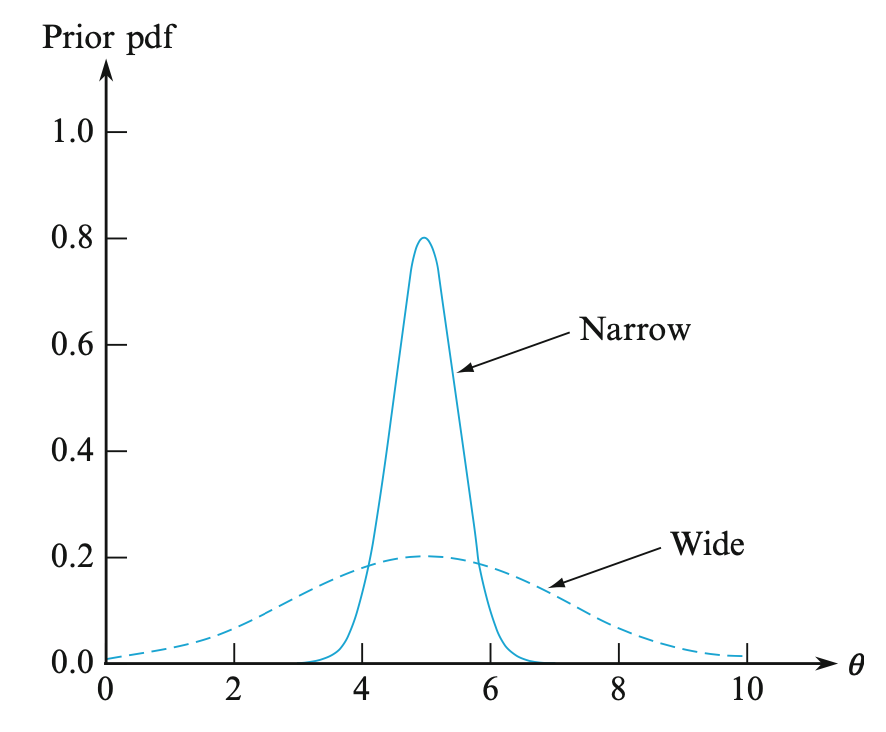
\includegraphics[scale=0.6]{./3_Images/prior_illustration.png}
%    \caption{A narrow concentrated prior about some central value and a wider less informative prior.}
%    \label{fig:prior_illustration}
%    \source{Figure 14.3 in \cite{STK}.}
%\end{figure}


\begin{figure}[H]
    \centering
    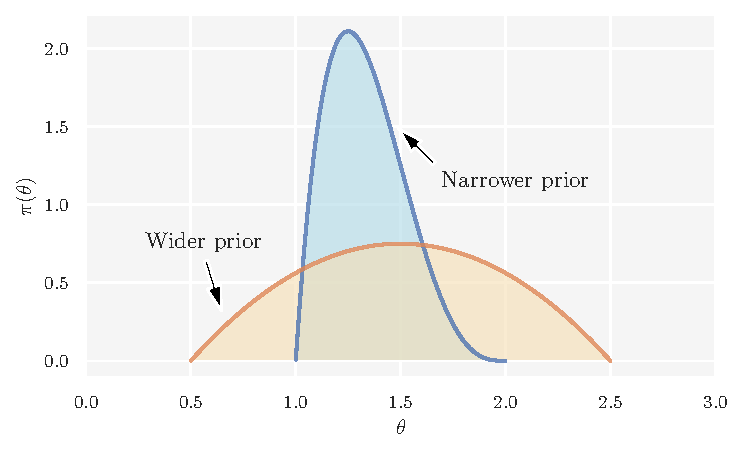
\includegraphics[scale=1.0]{prior_plot}
    \caption{Two prior distributions $\pi (\theta)$. A narrow concentrated prior (more certainty) about some central value and a wider less informative prior (less certainty).}
    \label{fig:prior_illustration}
    %\source{Figure 14.3 in \cite{STK}.}
\end{figure}

Our prior state of knowledge is modified by data $y$, obtained by performing experiments, through the conditional \textit{sampling distribution} $\lhood$. When regarded as a function of $\theta$, for fixed $y$, $\lhood$ is called the \textit{likelihood function}. In order to make probability statements about $\theta$ given sample data $y$, a probabilistic model representing the joint probability distribution for $\theta$ and $y$ must be provided. The joint pmf or pdf can be written as a product of the prior distribution $\prior$ and the likelihood function $\lhood$:

\begin{equation*}
    \joint = \lhood \prior .
\end{equation*}

At this point, Bayes' theorem is used to produce the \textit{posterior distribution}, which represents our state of knowledge about $\theta$ in the light of $y$. A common incarnation of Bayes' theorem is:

\begin{equation}\label{eq:bayes_theorem}
    \posterior = \frac{\joint}{p(y)}  = \frac{\lhood \prior}{p(y)},
\end{equation}

where the marginal probability of the data $p(y) = \int \lhood \prior \dd \theta$ in the case of continuous parameters, or, in the case of a discrete set of parameters, $p(y) = \sum_\theta \lhood \prior$, where the sum is over all possible values of $\theta$.

$p(y)$ is the same for all possible $\theta$, as it does not depend on $\theta$. With fixed $y$, this factor can thus be omitted in parameter inference since it constitutes a normalizing constant and does not enter into determining the relative posterior probabilities of different values of $\theta$. Omitting the factor $p(y)$ yields the unnormalized posterior distribution: 

\begin{equation}\label{eq:bayes_unnorm}
    \posterior \propto p(\theta, y) =  \lhood \prior .
\end{equation}

In this formulation, $\lhood$ is taken as a function of $\theta$ and not $y$.  

The core of Bayesian inference is encapsulated in \autoref{eq:bayes_theorem} and \autoref{eq:bayes_unnorm}. The principal task is to develop the joint probability model $\joint$ and perform the computations to obtain the posterior $\posterior$.

%The core of Bayesian inference is encapsulated in \autoref{eq:bayes_theorem} and \autoref{eq:bayes_unnorm}. The principal task is to develop the joint probability model $\joint$ and perform the computations to summarize the posterior $\posterior$.


%================================================================
%\section{Prior and Posterior Predictive Distributions}\label{sec:predictive}
%\section{Single-parameter Models}\label{sec:single_inference}
%================================================================  



%================================================================
\section{Parameter Inference}\label{sec:param_inference}
%\section{Single-parameter Models}\label{sec:single_inference}
%================================================================  

The way in which Bayes' theorem operates is best seen through examples. In the following we discuss Bayesian inference in the context of statistical models where closed forms are available. Such models are sometimes unrealistic, but their analysis often provides a useful starting point when it comes to constructing more realistic models. The focus of this section will be on how we can summarize the obtained posteriors with various graphical checks and numerical measures. 

%The way in which Bayes’s theorem operates is best seen through examples. In the following we develop some problem formulations to apply Bayesian analysis on for parameter inference. We will focus on situations where closed forms are available, that is, situations where we can use probability models based on the standard distributions. In particular, we will look at probability models based on the binomial and normal distributions. The binomial distribution is motivated from counting exchangeable outcomes, and the normal distribution applies to a random variable that is the sum of many exchangeable or independent terms. Such models are sometimes unrealistic, but their analysis often provides a useful starting point when it comes to constructing more realistic models. The toy problems developed in this section will later serve as benchmark problems. 

%================================================================
\subsection{The Beta-Binomial Model and the Effect of Priors}\label{sec:coin_flipping}
%===============================================================

The beta-binomial model is one of the simplest Bayesian models, and useful for introducing important concepts and computational methods in Bayesian analysis. The model is often illustrated in the context of the classical coin-flipping problem, where only a single scalar parameter, the success probability $\theta$, is to be estimated. 

In the coin-flipping problem, we toss a coin $n$ times and record the observations: either \textit{heads} or \textit{tails}. Based on this data, we try to answer questions such as \textit{is the coin fair?} Or, more generally, \textit{how biased is the coin?} In order to estimate the bias of a coin in a Bayesian setting, we need observed data, a probabilistic model of the data generating process, i.e., the likelihood, and a prior placed on the unknown model parameter. For this example, we assume that the data-gathering part is already done and we have recorded the number of heads after a number of coin flips. The bias of the coin is represented by the $\theta$ parameter, and we say that a coin with $\theta=1$ will always land heads, one with $\theta=0$ always tails and one with $\theta=0.5$ has an equal chance of landing either heads or tails. Assuming that only two outcomes are possible, heads or tails, and the random variable \textit{coin toss} is independent and identically distributed (iid), a candidate for the likelihood is the binomial distribution: 

% p \qty(y \mid \theta)
\begin{equation}\label{eq:coin_flip_likelihood}
    \lhood = \binom{n}{y} \theta^y \qty(1 - \theta)^{n-y}.
\end{equation}

This is a discrete distribution returning the probability of getting $y$ heads (or in general, successes) out of $n$ coin tosses (or in general, trials or experiments) given a fixed value of $\theta$ (probability of success). 

\autoref{fig:binom_distribution} illustrates the binomial distribution for different $\theta$. From the figure we see that $\theta$ indicates how likely it is to obtain a head when tossing a coin, making the binomial distribution a reasonable choice for the likelihood. 

\begin{figure}[ht]
    \centering
    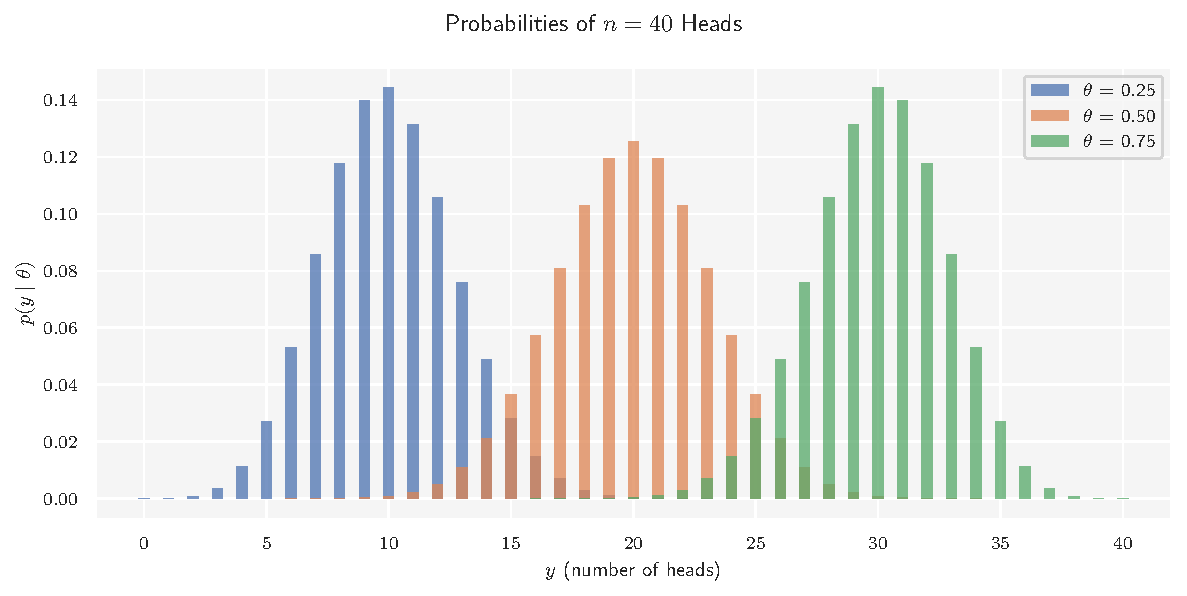
\includegraphics[scale=1]{binomial_distribution}
    \caption{Binomial distributions with $n=40$ coin flips and different success probabilities $\theta$. The coin is biased towards tails when $\theta < 0.5$ (blue) and heads when $\theta > 0.5$ (green). For $\theta=0.5$ (orange) the coin is unbiased (or fair). The legend indicates the values of the $\theta$.}
    \label{fig:binom_distribution}
\end{figure} 

If the value of $\theta$ is known, the binomial distribution tells us the expected distribution of heads. However, $\theta$ is an unknown model parameter, and thus we need to place a prior on it. For mathematical convenience, we choose a family of prior densities that lead to simple posterior densities. Considered as a function of $\theta$, \autoref{eq:coin_flip_likelihood} is of the form: 
\begin{equation*}
    \lhood \propto \theta^a \qty(1 - \theta)^b.
\end{equation*} 

If the prior density is of the same form, with its own parameterization of $a$ and $b$, then the posterior will also be of this form. Such a prior density can be parameterized as: 

\begin{equation*}
    \prior \propto \theta^{\alpha - 1} \qty(1 - \theta)^{\beta -1},
\end{equation*}

which is the beta distribution with shape parameters $\alpha>0$ and $\beta>0$. The parameters of the prior distribution are often called \textit{hyperparameters}. In order to ensure that the total probability is 1, the beta function,

\begin{equation*}
    B (\alpha, \beta) = \frac{\Gamma(\alpha)\Gamma(\beta)}{\Gamma(\alpha + \beta)},
\end{equation*}

where $\Gamma (z)$ is the gamma function, can be used as a normalizing constant:

\begin{equation}\label{eq:beta_prior}
    \prior = \frac{1}{B(\alpha, \beta)} \theta^{\alpha -1} (1-\theta)^{\beta -1}.
\end{equation}

The beta distribution is defined on the interval $[0, 1]$. \autoref{fig:beta_distribution} shows the beta distribution with different shape parameters. The figure displays the versatility of the beta distribution; the distribution adopts several shapes, determined by the shape parameters, including the uniform distribution with $\alpha = \beta = 1$. The uniform (blue) prior represents all the possible values for $\theta$ being equally likely a priori. The Gaussian-like (orange) prior is concentrated about $\theta=0.5$, and reflects a belief that the coin is equally probable to land heads or tails. The reverse J-shaped (green) prior is skewed towards a tail-biased outcome.

\begin{figure}[ht]
    \centering
    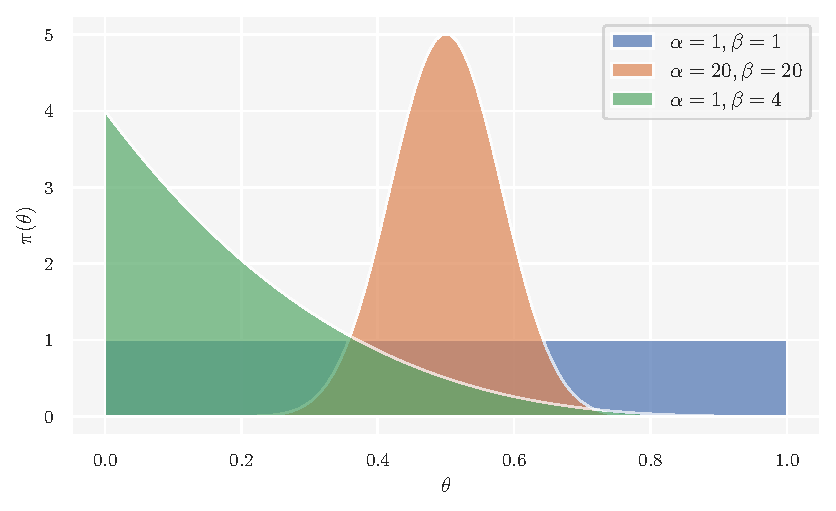
\includegraphics[scale=1]{beta_distribution}
    \caption{The beta prior probability distribution with different parameterizations by the two positive shape parameters. The beta distribution adopts several shapes controlled by the shape parameters; $\alpha=\beta=1$ gives a uniform distribution (blue), $\alpha=\beta=20$ gives a bell curve centered at $\theta=0.5$ (orange) and finally $\alpha=1$ and $\beta=2$ gives a reverse J-shaped distribution with a right tail (green).
    }
    \label{fig:beta_distribution}
\end{figure} 


Bayes' theorem, \autoref{eq:bayes_unnorm}, states that the posterior is proportional to the product of the likelihood and the prior. Thus, for our problem the posterior density for $\theta$ is given as: 

\begin{equation*}
    \pi (\theta \mid y) \propto \binom{n}{y} \theta^y (1-\theta)^{n-y} \frac{1}{B(\alpha, \beta)} \theta^{\alpha-1}(1-\theta)^{\beta -1}.
\end{equation*}

With fixed $n$ and $y$, the factor $\binom{n}{y}$ does not depend on the unknown parameter $\theta$, and neither does the beta function $B(\alpha, \beta)$. Thus can both be treated as constants when calculating the posterior distribution of $\theta$:

\begin{align*}
    \posterior &\propto \theta^y (1-\theta)^{n-y} \theta^{\alpha-1}(1-\theta)^{\beta -1} \\
    &= \theta^{\alpha + y -1} (1-\theta)^{\beta + n-y -1},
\end{align*}

or, more concisely:

\begin{equation}\label{eq:coin_posterior}
    \posterior \propto \theta^{\alpha' -1} (1-\theta)^{\beta' -1},
\end{equation}

with $\alpha'=\alpha+y$ and $\beta' = \beta + n - y$. We recognize that the expression above has the same functional form as the unnormalized beta distribution. The property that the posterior distribution follows the same parametric form as the prior distribution is called \textit{conjugacy}, and we say that the beta distribution is a \textit{conjugate prior} for the binomial likelihood.  

\autoref{fig:coin_flip_posterior} shows how the posteriors for the priors in \autoref{fig:beta_distribution} evolve as more and more data become available. For easier comparison, they have all been scaled vertically to have the same maximum value. \autoref{fig:coin_flip_posterior} clearly reveals the effect of the different priors; when there are few data, the shape of the posteriors vary in detail; as the number of data increases, the shape and location of the posteriors tend to converge and they all become sharply peaked. Since the priors reflect the different information or assumptions before the results, and the posteriors the updated knowledge in the light of data, this seems quite reasonable. If the data only are the outcome of a few flips, the analysis of these data is dominated by the prior information. However, as the data increases, the posterior is dominated by the likelihood and we are eventually led to the same conclusions regardless of our initial beliefs. In the limit of infinite data, all priors will provide the same posterior. From a practical point of view, we could obtain nearly indistinguishable posteriors for a finite amount of data. Thus, the choice of the prior becomes largely irrelevant given a sufficiently large amount of data.

\begin{figure}[H]
    \centering
    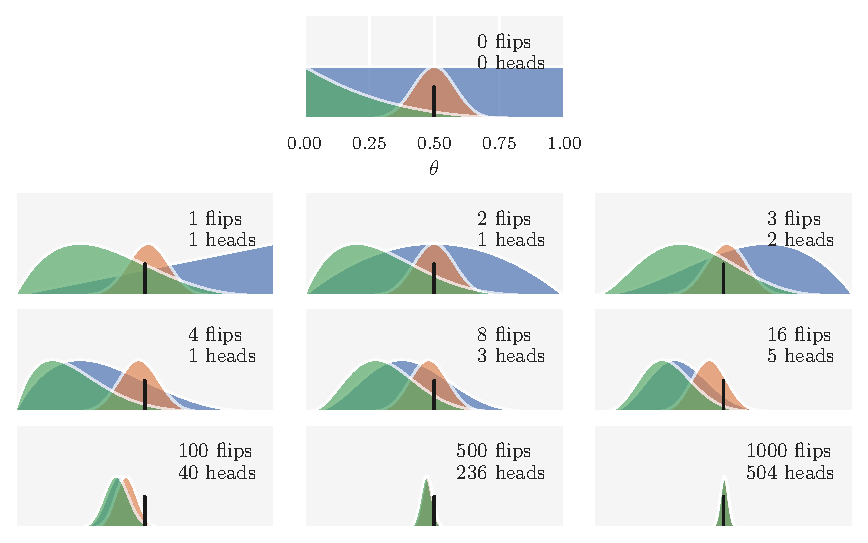
\includegraphics[scale=1]{coin_flip_posterior}
    \caption{The effect of different priors on the posterior as the number of data available increases. To aid in the comparison, they have all been scaled vertically to have the same maximum value. The number of data analyzed is indicated at the upper right-hand corner of each panel. In the first panel there are zero flips, and thus the densities represent the priors from \autoref{fig:beta_distribution}. The ground truth, $\theta=0.5$ (the coin is indeed fair), is indicated by the black vertical line. 
    }
    \label{fig:coin_flip_posterior}
\end{figure} 

 
Non-, weakly and informative priors. 

\url{http://www.stat.columbia.edu/~gelman/research/published/p039-_o.pdf}

An informative prior expresses specific, definite information about a variable. (then an example that I didn't understand).

An uninformative prior or diffuse prior expresses vague or general information about a variable. The term "uninformative prior" is somewhat of a misnomer. Such a prior might also be called a not very informative prior, or an objective prior, i.e. one that's not subjectively elicited. Uninformative priors can express "objective" information such as "the variable is positive" or "the variable is less than some limit".

%Two further curious points may be noted: (i) it takes quite a lot of flips to be able to estimate the bias-weighting with some degree of confidence (about a thousand to pin it down between 0.2 and 0.3); (ii) the posterior pdfs for the solid and dotted lines converge together quite quickly, but the dashed case takes much longer. The answer to the first observation is that it just does, but the number of flips required will depend on the actual bias-weighting of the coin. If the coin was tossed ten times and came up tails on every occasion, we would rapidly conclude that it was biased; on the other hand, the result of 45 heads and 55 tails in a hundred flips would still leave us somewhat uncertain as to whether the coin was fair. With regard to the second point, both the flat (solid) and the spiky (dotted) priors encode a large degree of ignorance about the nature of the coin. Despite the peculiar shape of the latter, it is fairly flat for most values of H; the strange-looking spikes at H = 0 and H = 1 disappear as soon as a head and a tail have been observed. The ‘fair-minded’ prior (dashed line), however, claims to be moderately well-informed about the character of the coin regardless of the data. It, therefore, takes much more to be convinced that the coin is not fair. Even though the prior probability for H = 0.5 was about a million times greater than that of H = 0.25, a thousand flips were enough to drag it (kicking and screaming, perhaps) to the conclusion that the value of H was less than 0.3 (but more than 0.2).

%non-, weakly and informative priors.

%These rules of thumb follow directly from the nature of the Bayesian analysis procedure:

%If the prior is uninformative, the posterior is very much determined by the data (the posterior is data-driven)

%If the prior is informative, the posterior is a mixture of the prior and the data

%The more informative the prior, the more data you need to "change" your beliefs, so to speak because the posterior is very much driven by the prior information

%If you have a lot of data, the data will dominate the posterior distribution (they will overwhelm the prior) 

%================================================================
%\section{Gaussian Models and Posterior Checks}\label{sec:gaussian_models}
\section{Summarizing the Posterior}
%\section{Summarizing the Posterior}
%================================================================ 

The result of a Bayesian analysis is a posterior distribution which contains all the current information about the parameters $\theta$. 


Commonly used summaries of location are the mean, median and mode(s) of the distribution; variation is commonly summarized by the standard deviation, the interquartile range and other quantiles. Each summary has its own interpretation: for example, the mean is the posterior expectation of the parameter, and the mode may be interpreted as the single 'most likely' value, given the data (and the model).


\subsection{Point estimates}

People often choose the median, just because it is more robust to outliers than the mean, or use the mean just because is a simple and familiar concept, or because they think their observable is truly the average of some process at some level, like molecules bouncing to each other or genes interacting with themselves and the environment.

\subsection{Posterior quantiles and intervals}







In principle, the posterior distribution contains all the information about the possible parameter values. In practice, we must also present the posterior distribution somehow. If the examined parameter  
θ
  is one- or two dimensional, we can simply plot the posterior distribution. Or when we use simulation to obtain values from the posterior, we can draw a histogram or scatterplot of the simulated values from the posterior distribution. If the parameter vector has more than two dimensions, we can plot the marginal posterior distributions of the parameters of interest.

However, we often also want to summarize the posterior distribution numerically. The usual summary statistics, such as the mean, median, mode, variance, standard devation and different quantiles, that are used to summarize probability distributions, can be used. These summary statistics are often also easier to present and interpret than the full posterior distribution.

THIS IS NEW

The result of a Bayesian analysis is a posterior distribution, and all the information about the parameters given a dataset and a model is contained in the posterior distribution. Thus, by summarizing the posterior, we are summarizing the logical consequences of a model and data. A common practice is to report, for each parameter, the mean (or mode or median) to have an idea of the location of the distribution and some measure, such as the standard deviation, to have an idea of the dispersion and hence the uncertainty in our estimate. The standard deviation works well for normal-like distributions but can be misleading for other type of distributions, such as skewed ones. So, an alternative is to use the following measure.

\subsection{Posterior Predictive Check}

To make inferences about an unknown variable, often called predictive inferences, we follow a similar logic. Before the data $y$ are considered, the distribution of unknown but observable $y$ is 

\begin{equation}\label{eq:prior_predictive}
    \pi (y) = \int \lhood \prior \dd{\theta}
\end{equation}

%BDA, side 7

Posterior predictive check
Comparing the data to the posterior predictions of the model is called a posterior predictive check. When there appear to be systematic discrepancies that would be meaningful to address, you should consider expanding or changing the model so it may be a better description of the data.

One way to evaluate whether the least unbelievable parameter values are any good is via a posterior predictive check. A posterior predictive check is an inspection of patterns in simulated data that are generated by typical posterior parameters values. The idea of a posterior predictive check is as follows: If the posterior parameter values really are good descriptions of the data, then the predicted data from the model should actually “look like” real data. If the patterns in the predicted data do not mirror the patterns in the actual data, then we are motivated to invent models that can produce the patterns of interest.

---

Posterior Predictive Distributions
For evaluating the fit of a model, perhaps the most flexible approach is to examine the Bayesian posterior predictive distribution. The posterior predictive distribution is the distribution of future observable data, based on the posterior distribution. It is defined as: 

eq same as 6.1 in BDA 

In this equation, $y_{rep}$ is future data that could be drawn from the posterior distribution, $y$ is the current data, and $\theta$ is the model parameter. Notice that the last two terms (prior to $d\theta$) are the posterior density for the parameter. The first term is the sampling density for future data, conditional on the parameter. This equation simply specifies a form for the distribution of future data, given the model parameter and data. If a model fits the current data well, then we expect that simulated future data should look much like the current data. Thus, we can simulate data from the posterior predictive distribution, compare it to the observed data, and determine whether the model has an appropriate fit. 

---

Following the same logic, prior predictive distribution  


\subsection{Measures of Predictive Accuracy}

Goodness of fit in Bayesian analyses is routinely assessed using a method referred to as the ‘Bayesian p-value’ and posterior predictive checks (Gelman et al., 1996).

s. 166/167 i BDA 

%================================================================
%\section{Gaussian Models and Posterior Checks}\label{sec:gaussian_models}
\subsection{Bayesian Analysis}
%\section{Summarizing the Posterior}
%================================================================


Posterior - all information

We will use a Gaussian model with unknown mean and variance to illustrate the following, since it is continuous and

The Bayesian Toolkit

One point that must be clear from the beginning is that the Bayesian approach is a complete inferential approach. Therefore, it covers confidence evaluation, testing, prediction, model checking, and point estimation. We will progres- sively cover the different facets of Bayesian analysis in other chapters of this book, but we address here the issue of confidence intervals because it is rather a straightforward step from point estimation.

normal models important blabla

As we saw in the previous section, conjugacy ensures tractable posteriors. Sufficent summary statistics, (mean and variance for normal)

The derivation requires some tedious algebra, so we simply state the result (Murphy, 07)

\url{https://en.wikipedia.org/wiki/Conjugate_prior#When_likelihood_function_is_a_continuous_distribution}


The comprehensive derivation can be found in appendix B. 

Devore, p. 781 

Note that the posterior mean $\mu_0'$ is a weighted average of the prior mean $\mu_0$ and the data mean $\bar{x}$, with weights that are the reciprocals of the prior variance and the variance of $\bar{x}$. It makes sense to define the \textbf{precision} as the reciprocal of the variance because a lower variance implies a more precise measurement and the weights then are the corresponding precisions. Furthermore, the posterior variance is the reciprocal of the sum of the reciprocals of the two variances, but this can be described much more simply by saying that the posterior precision is the sum of the prior precision plus the precision of $\bar{x}$.  


Sufficient statistics are useful in algebraic manipulations of likelihoods and posterior distributions.

sufficient summary statistics, lfi for cogsci, side 16, Fisher-Neyman Factorization Theorem

\url{https://bookdown.org/mrwhalen/bayes_book/summarizing-posterior-distributions.html}

Summarizing Posterior Distributions
Obtaining a posterior distribution is great, but does not provide us with much concrete to discuss or convey to others. Therefore, we need ways to distill the distribution into point estimates, or summary statistics. The most common summary statistics for posterior distributions will be the posterior mean, posterior mode and posterior median.

At times, there will be different reasons to use each summary statistic, but most often a safe assumption is to report the posterior mean $\pm$ posterior standard devition.

From a decision theory standpoint there technically are mathematical ways to determine which point estimate is the best to use in certian instances, but that is beyond the scope of this tutorial. However, here are the answers that come from magic (maybe I will post the proofs in the appendix:

1. If the loss function is quadratic, the best estimate is the posterior mean.
2. If the loss function is an absolute loss, the best estimate is the posterior median.
3. If the loss function is an All-or-nothing loss, the best estimate is the posterior mode

The posterior mode is just the expected value of the parameter estimate, using the posterior distribution.

Recall that a mode is simply the most frequent point in a data set. In a Bayesian distribution, this refers to the peak of the distribution (the parameterestimate with the highest overall weight). 

The posterior median refers to the value which divides the distribution in half. This is a bit more challenging to calculate by hand (and is the least frequently used summary statistic) but it is worth seeing where this value comes from.

We need to find the value $\theta$ which has 50\% of the probability to the left and 50\% to the right. It is also worth noting that the median is tricky to calculate for discrete distributions (hence why it is rarely seen).


Credible Intervals

There is a lot to say about the difference between Bayesian Credible Intervals and Classical Confidence Intervals. I will avoid this entire discourse and just say that in Bayesian statistics a Credible Interval is the interval in which we have a 95\% probabilistic belief the parameter is in that interval.

In Chapter 1, Thinking Probabilistically, we introduced the concept of posterior predictive checks, and, in subsequent chapters, we have used it as a way to evaluate how well models explain the same data that's used to fit the model. The purpose of posterior predictive checks is not to dictate that a model is wrong; we already know that! By performing posterior predictive checks, we hope to get a better grasp of the limitations of a model, either to properly acknowledge them, or to attempt to improve the model. Implicit, in the previous statement is the fact that models will not generally reproduce all aspects of a problem equally well. This is not generally a problem given that models are built with a purpose in mind. A posterior predictive check is a way to evaluate a model in the context of that purpose; thus, if we have more than one model, we can use posterior predictive checks to compare them.

%================================================================
%\section{Summarizing the Posterior}
%================================================================

In Bayesian inference, posterior beliefs about parameters are updated according to \textit{Bayes' theorem} upon observing data.  

The mean of this posterior distribution gives a point estimate of $\theta$. 

An interval having a posterior probability $.95$ gives a $95\%$ \textit{credibility} interval, an interval within which an unobserved parameter value falls with a particular probability, the Bayesian analogue of a $95\%$ confidence interval \cite[p. 777]{STK}.

Credible intervals 

HDI 

Energy

- mean, median, mode: point estimates

- variance and standard deviation: spread -> uncertainty 

- credible intervals, highest density posterior (hdp) 


RMSE, true value, SEM 

In practice, we generally do not have the value of the true parameter $\theta$ at hand. Instead, we have an estimation in the form of a posterior distribution. Thus, what we can do is find out the value of $\hat{\theta}$ that minimizes the expected loss function. By expected loss function, we mean the loss function averaged over the whole posterior distribution. 

%================================================================
%\subsubsection{With Unknown Mean and Variance}
%================================================================

%The comprehensive derivation can be found in appendix B. 




%================================================================
%\section{The Influence of the Prior and How to Choose One}\label{sec:prior}
%================================================================

%\url{http://www.stat.columbia.edu/~gelman/research/published/p039-_o.pdf}

%\begin{itemize}
%    \item Flat
%    \item Uninformative
%    \item Diffuse
%    \item The Jeffreys’ Prior: Suppose we cannot easily find the natural scale on which the likelihood is in data-translated format, or that such a decomposition does not exist. Jeffreys (1961) proposed a general prior in such cases, based on the Fisher information I of the likelihood. 
%    \item When a prior distribution is not integrable it is said to be \textit{improper}
%\end{itemize}


%================================================================
%\subsection{Conjugate Prior Distributions}
%================================================================

%In Bayesian probability theory, if posterior distributions are in the same family as the prior distributions, then both prior and posterior are called conjugate distributions and the prior is called conjugate prior.

%Conjugacy is formally defined as follows. If $\mathcal{F}$ is a class of sampling distributions $p \left(y | \theta \right)$, and $\mathcal{P}$ is a class of prior distributions for $\theta$, then the class $\mathcal{P}$ is \textit{conjugate} for $\mathcal{F}$ if

%\begin{equation}
%    \pi \left(\theta | y \right) \in \mathcal{P} \, \forall p \left(\cdot | \theta \right) \in \mathcal{F} \land \pi (\cdot) \in \mathcal{P}
%\end{equation}

%This definition is formally vague since if we choose $\mathcal{P}$ as the class of all distributions, then $\mathcal{P}$ is always conjugate no matter what class of sampling distributions is used. We are most interested in \textit{natural} conjugate prior families, which arise by taking $\mathcal{P}$ to be the set of all densities having the same functional form as the likelihood \cite{ABC_ch1}.

%A conjugate prior of a likelihood is a prior that, when used in combination with a given likelihood, returns a posterior with the same functional form as the prior. cite BAP

%================================================================
%\section{Prior and Posterior Predictive Checks}
%================================================================

%\begin{itemize}
    %\item \url{https://docs.pymc.io/notebooks/posterior_predictive.html}
    %\item \url{https://avehtari.github.io/masterclass/slides_ppc.pdf}
    %\item \url{https://vasishth.github.io/bayescogsci/book/sec-priorpred.html}
    %\item \url{https://betanalpha.github.io/assets/case_studies/principled_bayesian_workflow.html#113_Prior_Predictive_Checks}
    %\item \url{http://bebi103.caltech.edu.s3-website-us-east-1.amazonaws.com/2018/tutorials/t6a_model_generation_and_prior_predictive_checks.html} python
%\end{itemize}

%================================================================
%\section{Uncertainty/Sensitivty Analysis in the Bayesian Paradigm}
%================================================================






%================================================================
%\subsection{The Prior and Posterior Predictive Distributions}\label{sec:predictive}
%================================================================

%BDA, side 7





%================================================================
%\section{Why Bayes?}
%================================================================

%End chapter with this? No, move to introduction
 
%================================================================
%\chapter{Inference Engines}\label{chap:infeng}
\chapter{Bayesian Computation}\label{chap:infeng}
%================================================================


%================================================================
\section{Inference Engines}
%================================================================ 

While conceptually simple, Bayesian methods can be mathematically and numerically challenging. The main reason is that the marginal likelihood, the denominator in Bayes' theorem (see equation 1.4), usually takes the form of an intractable or computationally-expensive integral to solve. For this reason, the posterior is usually estimated numerically using algorithms from the Markov Chain Monte Carlo (MCMC) family or, more recently, variational algorithms. These methods are sometimes called inference engines, because, at least in principle, they are capable of approximating the posterior distribution for any probabilistic model. 

There are several methods to numerically compute the posterior. I have ordered them into two broad groups: Non-Markovian methods (Grid computing, Quadratic approximation, Variational methods) and Markovian methods (Metropolis-Hastings, Hamiltonian Monte Carlo, Sequential Monte Carlo). We will not discuss non-Markovian methods as the focus of this thesis is MCMC methods.

%================================================================
\subsection{Markov Chain Monte Carlo Methods}
%================================================================ 



There is a family of related methods, collectively known as MCMC methods. These stochastic methods allow us to get samples from the true posterior distribution as long as we are able to compute the likelihood and the prior point-wise. While this is the same condition that we need for the grid-approach, MCMC methods outperform the grid approximation. The is because MCMC methods are capable of taking more samples from higher-probability regions than lower ones. In fact, an MCMC method will visit each region of the parameter-space in accordance to their relative probabilities.

To understand what MCMC methods are, we are going to split the method into the two MC parts; the Monte Carlo part and the Markov Chain part.

%================================================================
\subsection{Diagnosing Markov Chains}
%\section{Diagnosing Posterior Samples}
%================================================================ 


%================================================================
\subsection{Other methods}
%\section{Diagnosing Posterior Samples}
%================================================================

NUTS

%================================================================
\section{Density Estimation}\label{sec:dens_est}
%================================================================

The probability density function (pdf) is a fundamental concept in statistics. In the following, we will discuss \textit{density estimation}, i.e., how to construct an estimate of the pdf from sample data. The likelihood-free inference methods are based on sampling parameters and estimating the posterior from the samples, and hence is density estimation a crucial topic to address. As we will see, density estimation can give representations that have qualitatively different features and lead to entirely different interpretation of the data. 

%================================================================
\subsection{Histograms}\label{sec:histograms}
%================================================================ 

The most basic density estimator is the histogram [1]. A histogram is an approximate representation of data that divides the data into discrete bins and counts the number of points that fall in each bin. In a more general mathematical sense, a histogram is defined as follows [1]. We denote the density estimator by $\hat{f}$ and assume we are given a sample of $n$ observations $X_1, ..., X_n$ whose underlying density is to be estimated. Given an origin $x_0$ and a bin width $h$, the bins of the histogram are defined as the intervals $[x_0 + mh, x_0 + (m+1)h)$ for $m$ positive and negative integers. The histogram is then defined by

\begin{equation*}
    \hat{f}(x) = \frac{1}{nh} \times (\text{no. of } X_i \text{ in the same bin as } x)
\end{equation*}

The histogram can be generalized by allowing the bin widths to vary. Then the estimate becomes 

\begin{equation*}
    \hat{f}(x) = \frac{1}{n} \times \frac{(\text{no. of } X_i \text{ in the same bin as } x)}{\text{width of bin containing }x}
\end{equation*}

For instance, if we create some data that is drawn from a mixture density of two normal distributions, a simple  histogram, that is normalized such that the height of the bins reflects density instead of counts and have equal-width bins, will give the following representation of the data: 

\begin{figure}[H]
    \centering
    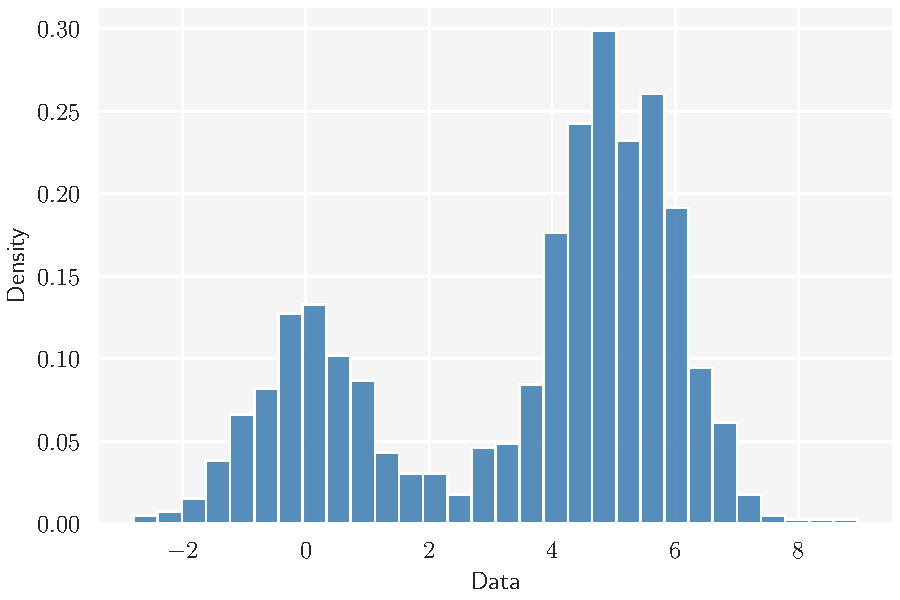
\includegraphics[scale=0.6]{bimodal_data.pdf}
    \caption{Density estimation by the histogram density estimator of 1000 observed data samples drawn from a mixed density of two normal distributions divided into 30 bins.}
    \label{fig:bimodal_data}
    \source{jakevdp book}
\end{figure}

The preceding figure illustrates why histograms are an immensely useful class of density estimates; they visualize data in an intuitive manner which is key for the presentation and exploration of data. The histogram makes clear that the data is drawn from a bimodal normal distribution.

One of the issues with using a histogram as a density estimator, however, is that the exact visual appearance depends on the choice of bin width (or number of bins) [2]. Different bin widths can give representations that have qualitatively different features and lead to entirely different interpretation of the data. Consider the following example where we draw 20 samples from the same distribution as before and use two histograms with different bin widths as density estimators:

\begin{figure}[H]
    \centering
    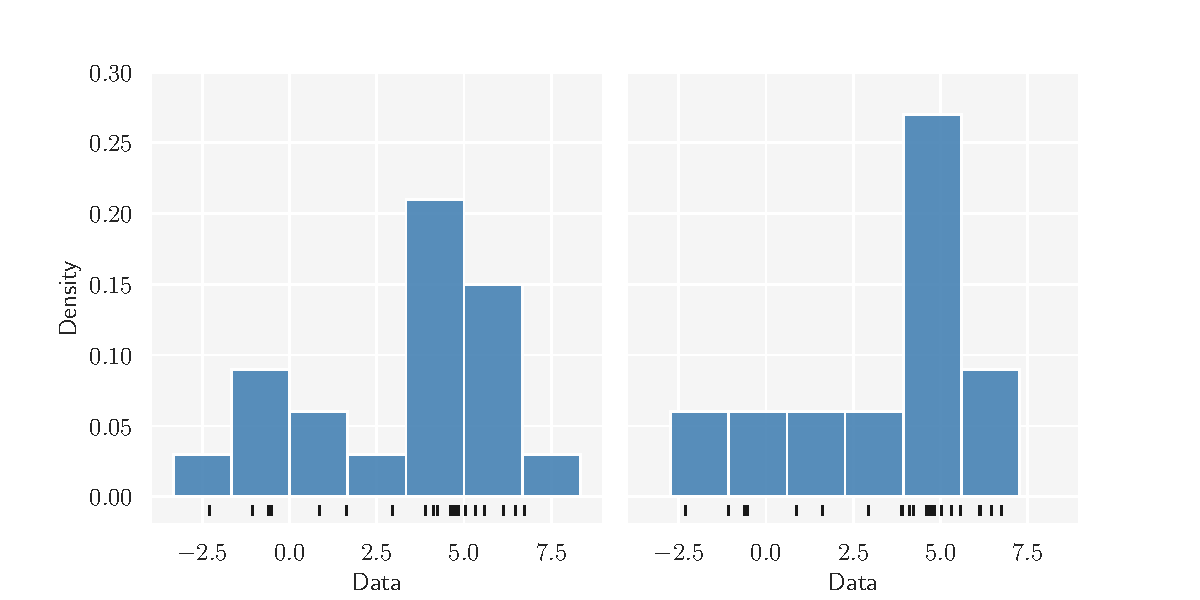
\includegraphics[scale=0.6]{bimodal_bins.pdf}
    \caption{These histograms are built from the same data, but with different bin widths. Together they illustrate one of the issues with using histograms as density estimators; the choice of bin widths can lead to vastly different representations of the data.}
    \label{fig:bimodal_bins}
    \source{jakevdp book}
\end{figure}

Without knowing that these two histograms were built from the same data, we probably would not have guessed so. The histogram on the left indicates a bimodal distribution as before, but the histogram on the right only shows a unimodal distribution with a long tail.   


%================================================================
\subsection*{Number of Bins and Width}\label{sec:binning}
%================================================================ 


There are no hard-and-fast rules concerning the bin width, and in extension the number of bins [3, p. 16]. The number of bins $k$ can be assigned directly or can be calculated from a suggested bin width $h$ as:

\begin{equation}
    k = \left \lceil \frac{\mathrm{max}\, x - \mathrm{min}\, x}{h} \right \rceil, 
\end{equation}

where $x$ is the sample data with $n$ observations. The braces indicate the ceiling function.

Smaller bin widths can make the histogram cluttered and larger bin widths may obscure nuances in the data. There are however some commonly-used rules-of-thumb, each of which has its own strengths and weaknesses. 

\subsubsection*{The Square-root Rule}

Generally, the larger the number of observations in the sample data, the more bins should be used [3, p. 16]. A reasonable rule of thumb is to take the square root of the number of observations in the sample and round to the next integer:

\begin{equation}
    k = \left \lceil \sqrt{n} \right \rceil 
\end{equation}

\textbf{Pros and Cons:} TODO

\subsubsection{Sturges' Rule}

\textbf{Rewrite, borrowed in it's entirety from Wikipedia}

Sturges' formula is derived from a binomial distribution and implicitly assumes an approximately normal distribution.

\begin{equation}
    k = \left \lceil \log_2 n \right \rceil + 1 
\end{equation}

It implicitly bases the bin sizes on the range of the data and can perform poorly if $n < 30$, because the number of bins will be small — less than seven — and unlikely to show trends in the data well. It may also perform poorly if the data are not normally distributed.

\subsubsection{Scott's Rule}

\begin{equation}
    h = \frac{3.49 \hat{\sigma}}{\sqrt[3]{n}},
\end{equation}

where $\hat{\sigma}$ is the sample standard deviation. Scott's normal reference rule is optimal for random samples of normally distributed data, in the sense that it minimizes the integrated mean squared error of the density estimate. 

\subsubsection{Freedman-Diaconis Rule}

\begin{equation}
    h = 2 \frac{\mathrm{IQR}(x)}{\sqrt[3]{n}},
\end{equation}

which is based on the interquartile range, denoted by $\mathrm{IQR}$. It replaces $3.5\sigma$ of Scott's rule with $2\,\mathrm{IQR}$, which is less sensitive than the standard deviation to outliers in data.

\subsubsection{Knuth's Rule}

Knuth's rule is a fixed-width, Bayesian approach to determining the optimal bin width of a histogram. The optimal number of bins is the value $M$ which maximizes the function 

\begin{equation}
    F(M \mid x, I) = n \log(M) + \log \Gamma \left(\frac{M}{2} \right) - \log \Gamma \left(\frac{1}{2} \right) - \log \Gamma \left(\frac{2n + M}{2} \right) + \sum_{k=1}^{M} \log \Gamma \left(n_k \frac{1}{2} \right),
\end{equation}

where $\Gamma$ is the gamma function, $n$ is the number of data points, $n_k$ is the number of measurements in bin $k$.


\begin{figure}[H]
    \centering
    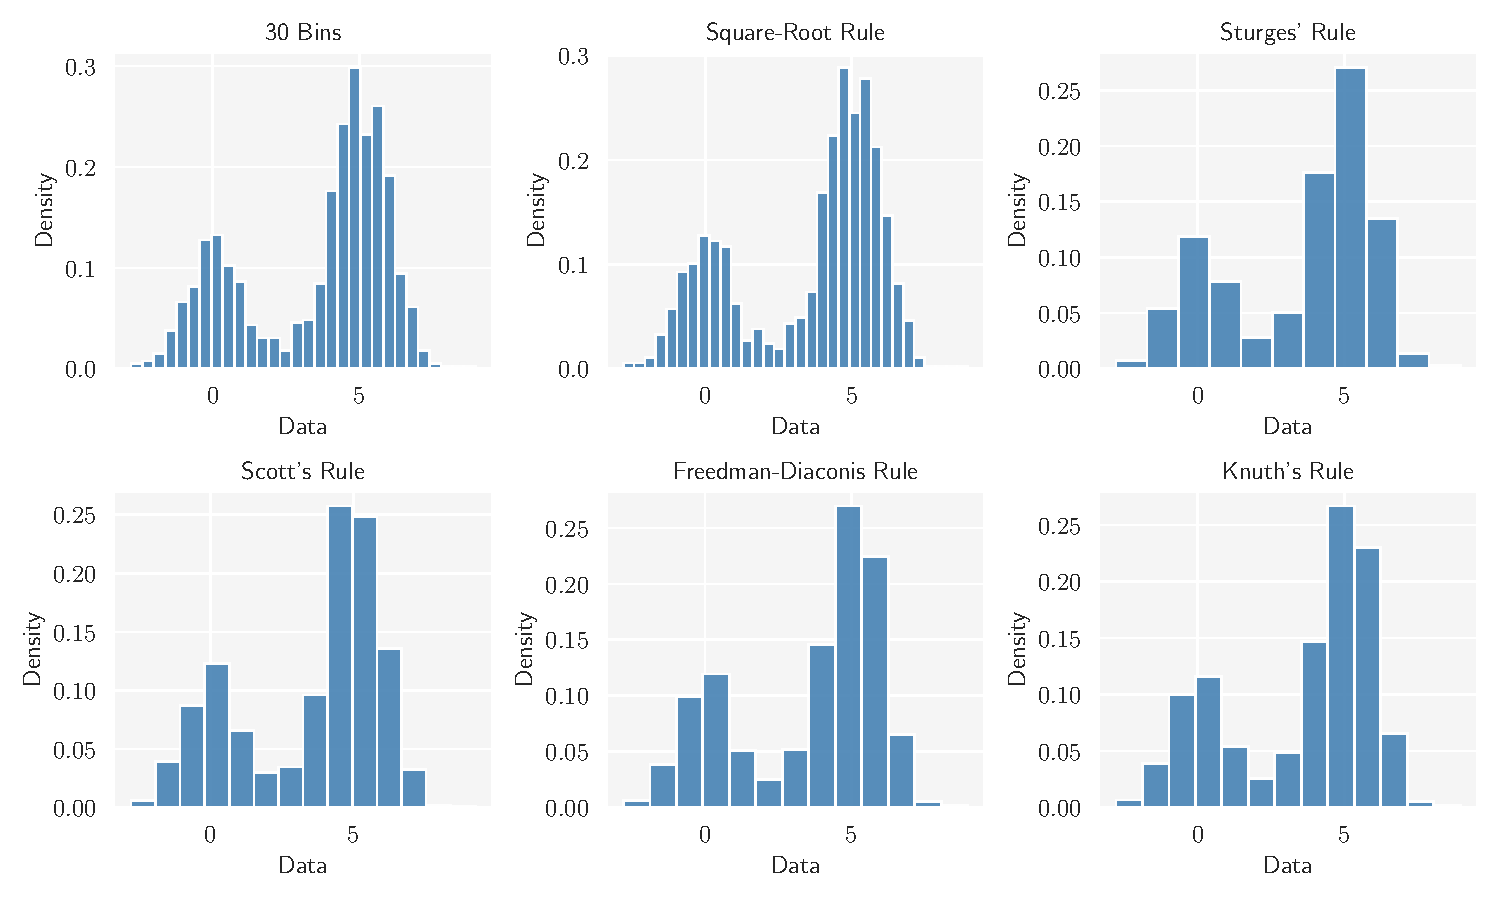
\includegraphics[scale=0.6]{histogram_rules.pdf}
    \caption{Histograms with binning as dictated by the rule specified in the subplot titles.}
    \label{fig:histogram_rules}
\end{figure}


\subsection*{References}

[1] \url{https://ned.ipac.caltech.edu/level5/March02/Silverman/paper.pdf}

[2] Python Data Science Handbook by Jake VanderPlas

[3] STK bok

[4] \url{https://clauswilke.com/dataviz/histograms-density-plots.html}

\subsubsection*{Original papers:} 

Scott, D. (1979). On optimal and data-based histograms \url{http://biomet.oxfordjournals.org/content/66/3/605}

Freedman, D. and Diaconis, P. (1981). On the histogram as a density estimator: L2 theory \url{http://www.springerlink.com/content/mp364022824748n3/}

\textbf{See also SNL thesis:} Primer on density estimation (parametric/non-parametric) and includes neural density estimators. 

\subsubsection*{Misc. sources:}

\begin{itemize}
    \item Python Data Science Handbook by Jake VanderPlas
    \item \url{https://clauswilke.com/dataviz/histograms-density-plots.html}
    \item \url{https://ned.ipac.caltech.edu/level5/March02/Silverman/paper.pdf}
    \item \url{http://users.stat.ufl.edu/~rrandles/sta6934/smhandout.pdf}
    \item \url{https://jakevdp.github.io/PythonDataScienceHandbook/04.05-histograms-and-binnings.html}
    \item \url{https://jakevdp.github.io/PythonDataScienceHandbook/05.13-kernel-density-estimation.html}
    \item \url{https://towardsdatascience.com/histograms-and-density-plots-in-python-f6bda88f5ac0}
    \item \url{https://seaborn.pydata.org/tutorial/distributions.html}
    \item \url{https://www.astroml.org/user_guide/density_estimation.html#kernel-density-estimation}
    \item \url{https://docs.astropy.org/en/stable/visualization/histogram.html#bayesian-models}
    \item \url{https://machinelearningmastery.com/probability-density-estimation/}
    \item \url{https://stackoverflow.com/questions/33458566/how-to-choose-bins-in-matplotlib-histogram/33459231}
    \item \url{https://stackoverflow.com/questions/30145957/plotting-2d-kernel-density-estimation-with-python}
\end{itemize}



\subsection*{Notes}

Histograms give a rough sense of the density of the underlying distribution of the data, and often for density estimation: estimating the probability density function of the underlying variable. The total area of a histogram used for probability density is always normalized to 1. If the length of the intervals on the x-axis are all 1, then a histogram is identical to a relative frequency plot.

A histogram can be thought of as a simplistic kernel density estimation, which uses a kernel to smooth frequencies over the bins. This yields a smoother probability density function, which will in general more accurately reflect distribution of the underlying variable. The density estimate could be plotted as an alternative to the histogram, and is usually drawn as a curve rather than a set of boxes. Histograms are nevertheless preferred in applications, when their statistical properties need to be modeled. The correlated variation of a kernel density estimate is very difficult to describe mathematically, while it is simple for a histogram where each bin varies independently. 

Though rules-of-thumb like Scott’s rule and the Freedman-Diaconis rule are fast and convenient, their strong assumptions about the data make them suboptimal for more complicated distributions. Other methods of bin selection use fitness functions computed on the actual data to choose an optimal binning. Astropy implements two of these examples: Knuth’s rule (implemented in knuth\_bin\_width()) and Bayesian Blocks (implemented in bayesian\_blocks()).

\url{https://docs.astropy.org/en/stable/visualization/histogram.html?fbclid=IwAR1qgq-CS2YLA3ui_03P9oRDcKiHXf7XE5lLYuglSjtLEXjtDSp7QBAKYag#bayesian-models}

\url{https://www.astroml.org/user_guide/density_estimation.html?fbclid=IwAR24wrXL_hTLJ8iLkzfMczUc7nUAc5elXgxpimT-A341NVaYuNKHJalXKsA#kernel-density-estimation}

\url{https://seaborn.pydata.org/tutorial/distributions.html?fbclid=IwAR3VjoNoDOcWeaERXvICVx_NL9DJ-tqhd1gBW6emPrrffgD1-0sZwtzn91I}


A rug plot is a plot of data for a single quantitative variable, displayed as marks along an axis. It is used to visualise the distribution of the data. As such it is analogous to a histogram with zero-width bins, or a one-dimensional scatter plot.

Rug plots are often used in combination with two-dimensional scatter plots by placing a rug plot of the x values of the data along the x-axis, and similarly for the y values. This is the origin of the term "rug plot", as these rug plots with perpendicular markers look like tassels along the edges of the rectangular "rug" of the scatter plot.

%================================================================
\subsection{Kernel Density Estimation}\label{sec:kde}
%================================================================

Histograms have been a popular visualization option since at least the 18th century, in part because they are easily generated by hand. More recently, as extensive computing power has become available in everyday devices such as laptops and cell phones, we see them increasingly being replaced by density plots. In a density plot, we attempt to visualize the underlying probability distribution of the data by drawing an appropriate continuous curve (Figure 7.3). This curve needs to be estimated from the data, and the most commonly used method for this estimation procedure is called kernel density estimation. In kernel density estimation, we draw a continuous curve (the kernel) with a small width (controlled by a parameter called bandwidth) at the location of each data point, and then we add up all these curves to obtain the final density estimate

Analogous to the binwidth of a histogram, a density plot has a parameter called the bandwidth that changes the individual kernels and significantly affects the final result of the plot. The plotting library will choose a reasonable value of the bandwidth for us (by default using the ‘scott’ estimate)

With many data points the rug plot can become overcrowded, but for some datasets, it can be helpful to view every data point. The rug plot also lets us see how the density plot “creates” data where none exists because it makes a kernel distribution at each data point. These distributions can leak over the range of the original data and give the impression that Alaska Airlines has delays that are both shorter and longer than actually recorded. We need to be careful about this artifact of density plots and point it out to viewers!


\url{https://github.com/COINtoolbox/CosmoABC/blob/master/cosmoabc/weighted_gaussian_kde.py} see set bandwidth function   
%================================================================
\chapter{Inference Engines}\label{chap:infeng}
%================================================================

While conceptually simple, Bayesian methods can be mathematically and numerically challenging. The main reason is that the marginal likelihood, the denominator in Bayes' theorem (see equation 1.4), usually takes the form of an intractable or computationally-expensive integral to solve. For this reason, the posterior is usually estimated numerically using algorithms from the Markov Chain Monte Carlo (MCMC) family or, more recently, variational algorithms. These methods are sometimes called inference engines, because, at least in principle, they are capable of approximating the posterior distribution for any probabilistic model. 

There are several methods to numerically compute the posterior. I have ordered them into two broad groups: Non-Markovian methods (Grid computing, Quadratic approximation, Variational methods) and Markovian methods (Metropolis-Hastings, Hamiltonian Monte Carlo, Sequential Monte Carlo). We will not discuss non-Markovian methods as the focus of this thesis is MCMC methods.

\section{Markov Chain Monte Carlo Methods}

There is a family of related methods, collectively known as MCMC methods. These stochastic methods allow us to get samples from the true posterior distribution as long as we are able to compute the likelihood and the prior point-wise. While this is the same condition that we need for the grid-approach, MCMC methods outperform the grid approximation. The is because MCMC methods are capable of taking more samples from higher-probability regions than lower ones. In fact, an MCMC method will visit each region of the parameter-space in accordance to their relative probabilities.

To understand what MCMC methods are, we are going to split the method into the two MC parts; the Monte Carlo part and the Markov Chain part.



%================================================================
\chapter{Likelihood-Free Inference}\label{chap:LFI}
%================================================================

Suppose a data-generating process is controlled by parameters $\theta$. When the process is run forward it stochastically generates a datapoint $y$ whose distribution depends on $\theta$. For every setting of $\theta$, assume that the process defines a conditional density function $\lhood$. Given an observed datapoint $y_0$ known to be generated by the process, the problem of interest is inferring plausible parameter settings that could have generated $y_0$. In particular, computing the posterior density $\pi \qty(\theta \mid y=y_0)$ obtained by Bayes theorem (\autoref{eq:bayes_theorem}) is of interest. The choice of inference algorithm primarily depends on how the data-generating process is modelled.
%\cite[p. 54]{papamakarios2019neural}. 

A purely statistical model, also known as a \textit{density model} or \textit{explicit model}, describes the conditional density function $\lhood$ of the process given values for $y$ and $\theta$. With a density model, the posterior density $\pi \qty(\theta \mid y=y_0)$ is, in general, easily evaluated using Bayes theorem. Even though the normalizing constant (or evidence) $p\qty(y_0)$ is typically intractable, samples from the posterior can be generated using a number of popular algorithms such as importance sampling and Markov chain Monte Carlo, or the posterior can be approximated with a more convenient distribution using e.g. variational inference. Such methods are referred to as \textit{likelihood-based inference methods}, as they explicitly evaluate the likelihood $\lhood$.
%\cite[p. 55]{papamakarios2019neural} \cite[p. 4]{abc_handbook}.

On the contrary, a \textit{simulator model}, also known as an \textit{implicit model}, describes how the process generates data. Many mechanical models are implicitly defined through simulator models, that is, as a set of dynamical equations and possibly a description of stochastic processes. For any parameter setting $\theta$, a simulator model can be run forward to generate independent samples from $\lhood$. Unlike for explicit density models, likelihoods are generally intractable or computationally infeasible for complex data-generating processes such as simulation-based models. The absence or complexity of the associated likelihood typically arise from it involving computationally expensive or intractable integrals, or that the simulator's internal states are unavailable. In order to perform inference in a simulator model, methods using simulations from the model rather than likelihood evaluations are needed. Such methods are referred to as \textit{likelihood-free inference methods}.
%\cite{SNL18} \cite{SNPE17} \cite[p. 55]{papamakarios2019neural}.

In general, likelihood-free methods are less efficient than likelihood-based methods as the former can require lots of simulations to produce accurate results. One of the principal topics of research in likelihood-free inference is how to obtain state-of-the-art results with fewer simulations. 
%\cite{comparison_snl_snpe}. 

%================================================================
\section{Approximate Bayesian Computation}\label{sec:abc}
%===============================================================

Approximate Bayesian Computation (ABC) constitutes a class of computational methods rooted in Bayesian statistics that can be used to evaluate posterior distributions of model parameters without having to explicitly calculate likelihoods. ABC methods approximate the likelihood function by assessing how likely it is the model could have produced the observed data, based on comparing synthetic data generated by the simulator to the observed data. The simulations that do not reproduce the observed data within a specified tolerance are discarded \cite{ABCprimer}.
%\cite[p. ix]{abc_handbook}.

ABC methods have been successfully applied to a wide range of real-world problems, and have also paved the way for a range of other likelihood-free approaches. However, even though ABC methods are mathematically well-founded, they inevitably make assumptions and approximations whose impact needs to be carefully assessed \cite{ABCprimer}. In the following, three types of ABC methods will be discussed: the vanilla \textit{rejection ABC}, and the more sophisticated variant \textit{Markov chain Monte Carlo (MCMC) ABC}.


%================================================================
\subsection{Rejection ABC}\label{sec:rejection_abc}
%================================================================

Given observed data $y_0$ and synthetic data $y$ generated by a simulator, let $\rho (\cdot, \cdot)$ be a distance metric (e.g., the Euclidean norm) defined in data space $\R^D$ and $\epsilon \geq 0$ be a tolerance. For small $\epsilon$, the ABC approximation to the posterior is 

\begin{equation}
    \pi \qty(\theta \mid y=y_0) \simeq \pi \qty(\theta \mid \rho \qty(y, y_0) \leq \epsilon)
\end{equation}


Rejection ABC is a rejection-sampling method for obtaining independent samples from the approximate posterior $ \pi \qty(\theta \mid \rho \qty(y, y_0) \leq \epsilon)$. It works by first sampling a set of parameters from the prior $\prior$, then simulating data under the model specified by the sampled parameters, and only accepting and retaining the sample if the distance between $y$ and $y_0$ is no more than $\epsilon$. The tolerance parameter $\epsilon$ controls the trade-off between estimation accuracy and computational efficiency. With sufficiently small $\epsilon$, and a sensible distance metric, the accepted samples follow the exact posterior more closely, though the algorithm accepts less often. On the other hand, the algorithm accepts more often with a large $\epsilon$, but the accepted samples will yield a replica of the prior.
%\cite[p. 58]{papamakarios2019neural} \cite{abc_handbook}. 

An issue with ABC in general is that the required number of simulations increases dramatically as $\epsilon$ becomes small. Moreover, likelihood-free inference also becomes challenging when the dimensionality of the data is large. A common approach to lessen this problem is to use lower-dimensional summary statistics, $S(y)$ and $S(y_0)$, that capture important features such as the mean and standard deviation, in place of raw data. %\cite{SNL18}. 
A further motivation for this approach is that real-world experiments often are interested in capturing summary statistics of the experimental data. A summary statistic that contains the same amount of information about model parameters as the whole dataset, is referred to as being a \textit{sufficient statistic} \cite{ABCprimer}. The acceptance criterion in the rejection ABC algorithm then becomes:

\begin{equation}
    \rho \qty(S(y), S(y_0))
\end{equation}

In \autoref{fig:abc_pipeline}, a conceptual overview of the rejection ABC algorithm is shown. 

\begin{figure}[H]
    \centering 
    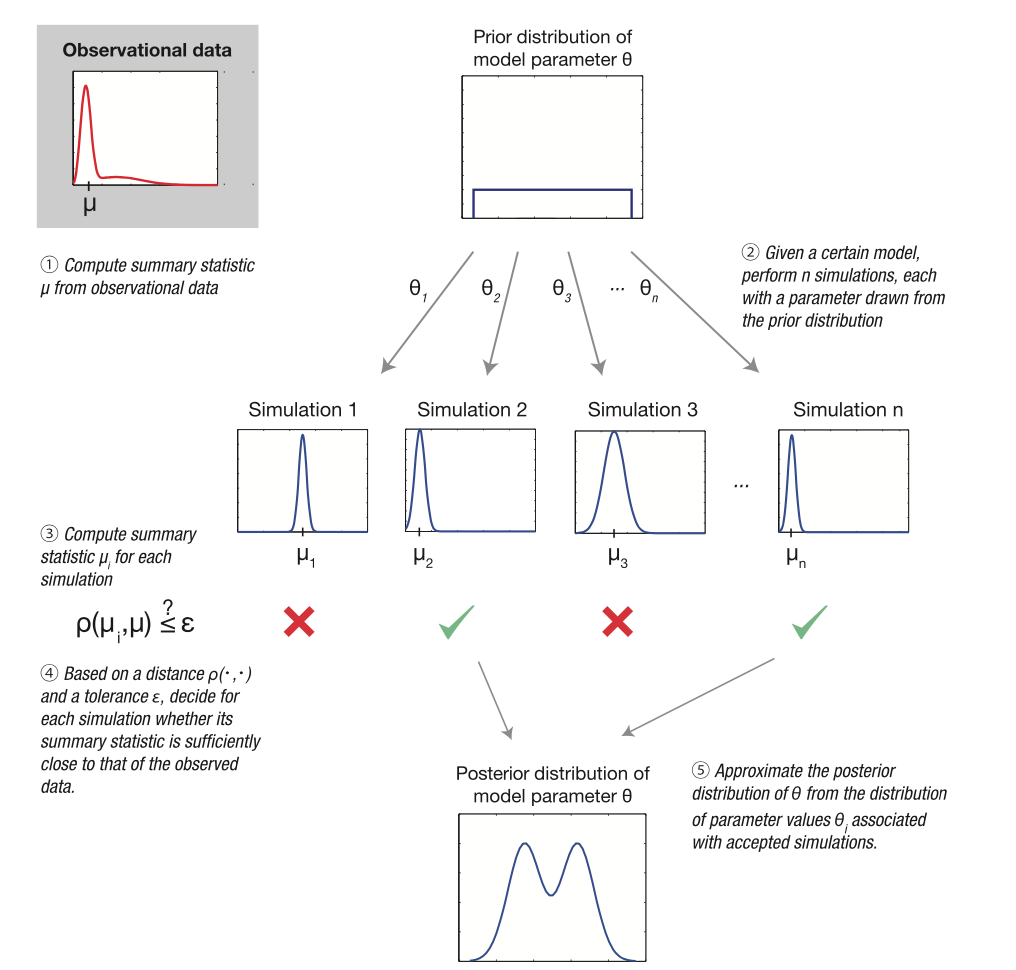
\includegraphics[scale=0.7]{./3_Images/abc_pipeline.png}
    \caption{Parameter estimation by Approximate Bayesian Computation: a conceptual overview.}
    \source{Figure 1 in \cite{ABCprimer}}
    \label{fig:abc_pipeline}
\end{figure}


%================================================================
\subsection{Markov Chain Monte Carlo ABC}\label{sec:mcmc_abc}
%================================================================

In the rejection ABC algorithm, parameters are sample from the prior $\prior$, and only parameters that are likely under the approximate posterior $\pi \qty(\theta \mid \rho \qty(y, y_0 ) \leq \epsilon )$ are accepted. The acceptance rate will be low if the approximate posterior is significantly narrower than the prior, as is often the case. %\cite[p. 59]{papamakarios2019neural}.

Markov-chain Monte Carlo (MCMC) ABC is an alternative approach that can lead to fewer rejections. Instead of proposing parameters from the prior, this method use the Metropolis-Hastings algorithm to propose new parameters $\theta'$ based on previously accepted parameters $\theta$ from the proposal density $q \qty(\theta' \mid \theta)$. By calculating the \textit{acceptance ratio}

\begin{equation}
    \alpha = \frac{p \qty(\rho \qty(y, y_0 ) \leq \epsilon \mid \theta') \pi\qty(\theta') q \qty(\theta \mid \theta')  }{p \qty(\rho \qty(y, y_0) \leq \epsilon \mid \theta) \pi\qty(\theta) q \qty(\theta' \mid \theta) },
\end{equation}

the algorithm outputs the proposed parameters $\theta'$ with probability $\min \qty(1, \alpha)$, otherwise it outputs the previous parameters $\theta$. 
%\cite[p. 59]{papamakarios2019neural}.

The approximate likelihood $p \qty(\rho \qty(y, y_0 ) \leq \epsilon \mid \theta)$ cannot be directly evaluated in the likelihood-free situation, but it can be estimated as the fraction of the simulated data $y$ whose distance from the observed data $y_0$ is no more than $\epsilon$:

\begin{equation}
    p \qty(\rho \qty(y, y_0) \leq \epsilon \mid \theta) \approx \frac{1}{N} \sum_n I \qty(\rho \qty(y_n, y_0) \leq \epsilon),
\end{equation}

where $y_n \sim p \qty(y \mid \theta)$ and $I(\cdot)$ is an indicator function. %\cite[p. 59]{papamakarios2019neural}.

Similarly to rejection ABC, the acceptance probability of MCMC ABC decreases as $\epsilon$ becomes small. Moreover, the performance of MCMC ABC strongly depends on the selection of proposal and prior density.

%================================================================
\subsection{Sequential Monte Carlo ABC}\label{sec:smc_abc}
%================================================================

TODO

%================================================================
\subsection{Population Monte Carlo ABC}\label{sec:pmc_abc}
%================================================================

TODO

\section{Notes}

\begin{itemize}
    \item See LFI for cognitive science book, Ch. 2.1
\end{itemize}

\textbf{Snippets:}

Although the steps listed above may give the impression that all likelihood- free algorithms are simple, this is unfortunately not the case. Many sophisticated techniques have been created in the hopes of increasing the efficiency of an algorithm on a given problem, and as one might expect, the efficiency of the algorithms below do vary by the type of problem to which they are applied. Because the algorithms we present later in this chapter are sometimes complex, we first introduce a few concepts at a high level by describing the different choices one can make at Steps 1, 2, or 3. 

The ABC methodology, where ABC stands for approxi- mate Bayesian computation, was mentioned as early as 1984 through a pedagogical and philosophical argument in Rubin (1984). It offers an almost automated resolution of the dif- ficulty with models which are intractable but can be simu- lated from. It was first proposed in population genetics by Tavaré et al. (1997), who introduced Approximate Bayesian Computation methods as a rejection technique bypassing the computation of the likelihood function via a simulation from the corresponding distribution. The exact version of the method can only be implemented in a small range of cases. Pritchard et al. (1999) produce a generalisation based on an approximation of the target. We study here the foundations as well as the implementation of the ABC method, with il- lustrations from time series. 

\textbf{Books/papers:} 

\begin{itemize}
    \item marin2012\_article\_abc, bra abc analyser 
\end{itemize}

LFI chapter, 2019 book statistics and data science, side 98, ligning (2): 

Unfortunately, we cannot evaluate (2) explicitly. However it is possible to drawn an IID random sample $T_N = \{ \Theta_j \}_{j=1}^N$ $(N \in \mathbb{N})$ from the quasi-posterior distribution that is characterized by (2), using the so-called rejection algorithm. 

\textbf{Links:}

\url{https://www.ncbi.nlm.nih.gov/pmc/articles/PMC4297650/}

Clearly, deciding how to characterize the data is an important choice in the likelihood-free context. Namely, it is impossible to know whether or not a set of statistics is sufficient for the unknown parameters if the likelihood is intractable.

\url{https://github.com/bmorris3/abc_interact/blob/master/abc_interact.ipynb}

\url{https://github.com/elfi-dev/elfi/blob/dev/elfi/methods/parameter_inference.py}

\textbf{MCMC} 

\url{https://github.com/davidtgonzales/ABC/blob/master/Lotka-Volterra%20ABC.ipynb}

\textbf{SMC} 

\url{https://docs.pymc.io/notebooks/SMC-ABC_Lotka-Volterra_example.html}

\url{https://github.com/pymc-devs/pymc3/tree/master/pymc3/smc}

\url{https://github.com/ICB-DCM/pyABC/blob/main/pyabc/inference/smc.py}

\url{https://github.com/vuolleko/abclib/blob/master/abclib.pyx}

\url{https://github.com/Neojume/pythonABC/blob/master/algorithms.py}


%================================================================
\section{The ABC of Approximate Bayesian Computation}\label{sec:abc_of_abc}
%================================================================

Content from notebook, source: ABC handbook

For discrete data $\mathcal{D}$, probability model $\mathcal{M}$ with parameters $\theta$ having prior $\pi(\theta)$, we can simulate observations from: 

\begin{equation}
    \pi (\theta \mid \mathcal{D}) \propto p(\mathcal{D} \mid \theta) \pi(\theta),
\end{equation}

via:

\begin{itemize}
    \item[A1] Generate $\theta \sim \pi(\theta)$
    \item[A2] Accept $\theta$ with probability proportional to the likelihood $p(\mathcal{D}\mid \theta)$
\end{itemize}
    
Algorithm A can be extended dramatically in its usefulness using the following, stochastically equivalent, version:

\begin{itemize}
    \item[B1] Generate $\theta \sim \pi(\theta)$
    \item[B2] Simulate an observation $\mathcal{D}'$ from model $\mathcal{M}$ with parameter $\theta$
    \item[B3] Accept $\theta$ if $\mathcal{D}' = \mathcal{D}$
\end{itemize}
    

While algorithms A and B are probabilistically identical, B is much more general in that one does not need to compute probabilities explicitly to make it work; only simulation is needed. Version B is due to Rubin (1984). 

The drawback of B is clear. It will typically be the case that for a given value of $\theta$, the chance of the outcome $\mathcal{D}'=\mathcal{D}$, namely $p(\mathcal{D} \mid \theta)$, is either vanishingly small or very time consuming to compute, resulting in an algorithm that does not work effectively. This is where ABC finally comes into play, in the form of the following scheme. We start with a discrepancy metric $\rho$ to compare datasets and a tolerance $\epsilon \geq 0$, and then: 

\begin{itemize}
    \item[C1] Generate $\theta \sim \pi(\theta)$
    \item[C2] Simulate an observation $\mathcal{D}'$ from model $\mathcal{M}$ with parameter $\theta$
    \item[C3] Compute $\rho \equiv \rho (\mathcal{D}', \mathcal{D})$, and accept $\theta$ as an appropriate draw from $\pi (\theta \mid \mathcal{D})$ if $\rho \leq \epsilon$
\end{itemize}
    
The parameter $\epsilon$ measures the tension between computability and accuracy. If $\rho$ is a metric, then 

\begin{equation*}
    \rho = 0 \quad \implies \quad \mathcal{D}'=\mathcal{D},
\end{equation*}

so that such an accepted $\theta$ is indeed an observation from the true posterior. 

Pritchard et al. (1999) were the first to describe a version of this scheme, in which the datasets in C3 were compared through a choice of summary statistics. Thus, $\rho$ compares how well a set of simulated summary statistics matches the observed summary statistics. If the statistics are sufficient for $\theta$, then when $\epsilon=0$, the accepted values of $\theta$ are still from the true posterior based on the full data. 

\textbf{This begs the question of how one might identify 'approximately sufficient' statistics, a topic covered in CHAPTER X.}

\subsection{Goodness of Fit}

\begin{itemize}
    \item Assessing performance 
    \item Expected quadratic loss
    \item \url{https://en.wikipedia.org/wiki/Loss_function}
    \item Expected loss
    \item In some contexts, the value of the loss function itself is a random quantity because it depends on the outcome of a random variable X.
    \item Both frequentist and Bayesian statistical theory involve making a decision based on the expected value of the loss function; however, this quantity is defined differently under the two paradigms.
\end{itemize}

\subsection{TODOs}

\begin{itemize}
    \item Sufficient vs insufficient statistics 
    \item $p(\theta \mid \rho (\hat{D}, D) \leq \epsilon)$ and $p(\theta |D)$ as a function of $\epsilon$. 
    \item The accuracy of the posterior (defined as the expected quadratic loss) delivered by ABC as a function of $\epsilon$
    \item Accuracy as a function of the number of data points in observed data
    \item KL divergence
    \item Accuracy vs number of posterior samples
\end{itemize}

%================================================================
\chapter{Introduction to Neurobiology}\label{chap:neuro}
%================================================================

The primary aim of this chapter is to introduce several elementary notions of neuroscience, in particular the concepts of action potentials, postsynaptic potentials, firing thresholds, refractoriness, and adaptation.

Due to the limitations of space we cannot – and do not want to – give a comprehensive introduction into such a complex field as neurobiology. The presentation of the biological background in this chapter is therefore highly selective and focuses on those aspects needed to appreciate the biological background of the theoretical work presented in this book. For an in-depth discussion of neurobiology we refer the reader to the literature mentioned at the end of this chapter. \url{https://neuronaldynamics.epfl.ch/online/Ch1.html}

In this chapter we go briefly through the physiology and (some function)(constituents) of biological brains.

%================================================================
\section{Elements of Neuronal Systems}
%================================================================

%================================================================
\section{The Brain}
%================================================================



%================================================================
\section{The Neuron}
%================================================================ 



%================================================================
\subsection{The Neuronal Membrane}
%================================================================ 

The cell body of every neuron is enclosed by a plasma \textit{membrane}. The electrical properties which underlie the membrane potential arise from the separation of intracellular and extracellular space by a cell membrane. The intracellular medium, cytoplasm, and the extracellular medium contain differing concentrations of various ions. Some key inorganic ions in nerve cells are: 

\begin{itemize}
    \item Positively charged \textit{cations}:
    \begin{itemize}
        \item $\mathrm{K}^+$, potassium
        \item $\mathrm{Na}^+$, sodium 
        \item $\mathrm{Ca}^{2+}$, calcium
        \item $\mathrm{Mg}^{2+}$, magnesium
    \end{itemize}
    \item Negatively charged \textit{anions}:
    \begin{itemize}
        \item $\mathrm{Cl}^-$, chloride
    \end{itemize}
\end{itemize}


Within the cell, the charge carried by anions and cations is usually almost balanced, and the same is true of the extracellular space. Typically, there is a greater concentration of extracellular sodium than intracellular sodium, and conversely for potassium. 

The key components of the membrane are: 

\textbf{Lipid bilayers:} The bulk of the membrane is composed of the 5 nm thick lipid bilayer. It is made up of two layers of lipids, which have their hydrophilic ends pointing outwards and their hydrophobic ends pointing inwards. It is virtually impermeable to water molecules and ions. This impermeability can cause a net build-up of positive ions on one side of the membrane and negative ions on the other. This leads to an electrical field across the membrane, similar to that found between the plates of an ideal electrical capacitor. 

\textbf{Ion channels:} are pores in the lipid bilayer, made of proteins, which can allow certain ions to flow through the membrane. Some ion channels are voltage gated, meaning that they can be switched between open and closed states by altering the voltage difference across the membrane. Others are chemically gated, meaning that they can be switched between open and closed states by interactions with chemicals that diffuse through the extracellular fluid. The ion materials include sodium, potassium, chloride, and calcium. The interactions between ion channels and ion pumps produce a voltage difference across the membrane, typically a bit less than 1/10 of a volt at baseline. This voltage has two functions: first, it provides a power source for an assortment of voltage-dependent protein machinery that is embedded in the membrane; second, it provides a basis for electrical signal transmission between different parts of the membrane.

--
WIKI:

Like all animal cells, the cell body of every neuron is enclosed by a plasma membrane, a bilayer of lipid molecules with many types of protein structures embedded in it. A lipid bilayer is a powerful electrical insulator, but in neurons, many of the protein structures embedded in the membrane are electrically active. These include ion channels that permit electrically charged ions to flow across the membrane and ion pumps that chemically transport ions from one side of the membrane to the other. Most ion channels are permeable only to specific types of ions. Some ion channels are voltage gated, meaning that they can be switched between open and closed states by altering the voltage difference across the membrane. Others are chemically gated, meaning that they can be switched between open and closed states by interactions with chemicals that diffuse through the extracellular fluid. The ion materials include sodium, potassium, chloride, and calcium. The interactions between ion channels and ion pumps produce a voltage difference across the membrane, typically a bit less than 1/10 of a volt at baseline. This voltage has two functions: first, it provides a power source for an assortment of voltage-dependent protein machinery that is embedded in the membrane; second, it provides a basis for electrical signal transmission between different parts of the membrane.

\subsubsection{1. What is the neuronal membrane made of?}

\textit{Lipid bilayers:} The bulk of the membrane is composed of the 5 nm thick lipid bilayer. It is made up of two layers of lipids, which have their hydrophilic ends pointing outwards and their hydrophobic ends pointing inwards. It is virtually impermeable to water molecules and ions. This impermeability can cause a net build-up of positive ions on one side of the membrane and negative ions on the other. This leads to an electrical field across the membrane, similar to that found between the plates of an ideal electrical capacitor.

\textit{Ion channels} are pores in the lipid bilayer, made of proteins, which can allow certain ions to flow through the membrane. 

\textit{Ionic pumps} are membrane-spanning protein structures that actively pump specific ions and molecules in and out of the cell. 

\subsubsection{3. What is meant by the resting membrane potential?}

There is an electrical potential difference across the cell membrane (difference between inside-outside of the neuron), called the \textit{membrane potential}. In neurons the membrane potential is used to transmit and integrate signals, sometimes over large distances. A resting (non-signaling) neuron has a voltage across its membrane called the \textit{resting membrane potential}. 

\subsubsection{4. How big is typically the resting membrane potential?}

The resting membrane potential is typically around -65 mV, meaning that the potential inside the cell is more negative than that outside.

\subsubsection{5. What are the key ions setting up the neuronal membrane potential and mediating electrical signals?}

Some key inorganic ions in nerve cells are: 

\begin{itemize}
    \item Positively charged \textit{cations}:
    \begin{itemize}
        \item $\mathrm{K}^+$, potassium
        \item $\mathrm{Na}^+$, sodium 
        \item $\mathrm{Ca}^{2+}$, calcium
        \item $\mathrm{Mg}^{2+}$, magnesium
    \end{itemize}
    \item Negatively charged \textit{anions}:
    \begin{itemize}
        \item $\mathrm{Cl}^-$, chloride
    \end{itemize}
\end{itemize}
    

Within the cell, the charge carried by anions and cations is usually almost balanced, and the same is true of the extracellular space. Typically, there is a greater concentration of extracellular sodium than intracellular sodium, and conversely for potassium. 

\subsubsection{6. What is an ion channel?}

\textit{Ion channels} are pores in the lipid bilayer, made of proteins, which can allow certain ions to flow through the membrane. Some ion channels are voltage gated, meaning that they can be switched between open and closed states by altering the voltage difference across the membrane. Others are chemically gated, meaning that they can be switched between open and closed states by interactions with chemicals that diffuse through the extracellular fluid. The ion materials include sodium, potassium, chloride, and calcium. The interactions between ion channels and ion pumps produce a voltage difference across the membrane, typically a bit less than 1/10 of a volt at baseline. This voltage has two functions: first, it provides a power source for an assortment of voltage-dependent protein machinery that is embedded in the membrane; second, it provides a basis for electrical signal transmission between different parts of the membrane.

\subsubsection{7. What are the two main categories of ion channels?}

Active and passive

\subsubsection{8. What is meant by an active channel?}

\textit{Active channels:} can exist in open states, where it is possible for ions to pass through the channel, and closed states, in which ions cannot permeate through the channel. Whether an active channel is in an open or closed state may depend on the membrane potential, ionic concentrations or the presence of bound ligands, such as neurotransmitters.

\subsubsection{9. What is meant by a passive channel?}

\textit{Passive channels:} In contrast, passive channels do not change their permeability in response to changes in the membrane potential. Sometimes a channel’s dependence on the membrane potential is so mild as to be virtually passive.

\subsubsection{10. What is an ion pump?}

\textit{Ionic pumps} are membrane-spanning protein structures that actively pump specific ions and molecules in and out of the cell. Particles moving freely in a region of space always move so that their concentration is uniform throughout the space. Thus, on the high concentration side of the membrane, ions tend to flow to the side with low concentration, thus diminishing the concentration gradient. Pumps counteract this by pumping ions against the concentration gradient.

\subsubsection{11. Which ion pump is particularly important for setting up the resting membrane potential?}

The sodium-potassium exchanger. The sodium–potassium exchanger pushes $K^+$ into the cell and Na$^+$ out of the cell. For every 2 K$^+$ ions pumped into the cell, 3 Na$^+$ ions are pumped out, a net outward current that makes the inside of the cell negative.

\subsubsection{12. What is an electrogenic pump?}


\textit{Electrogenic pump:} An ion pump that generates net flow of charge. This requires energy, which is provided by the hydrolysis of one molecule of adenosine triphosphate (ATP), a molecule able to store and transport chemical energy within cells.

The sodium–potassium exchanger is an electrogenic pump, as it genereates a net loss of charge in the neuron. 

An example of a pump which is not electrogenic is the sodium–hydrogen exchanger, which pumps one H$^+$ ion out of the cell against its concentration gradient for every Na$^+$ ion it pumps in. In this pump, Na$^+$ flows down its concentration gradient, supplying the energy required to extrude the H$^+$ ion; there is no consumption of ATP.





%================================================================
\section{Action Potentials}
%================================================================ 

\subsubsection{Action Potentials 1}

Action potentials are nerve signals. Neurons generate and conduct these signals along their processes in order to transmit them to the target tissues. Upon stimulation, they will either be stimulated, inhibited, or modulated in some way

An action potential is caused by either threshold or suprathreshold stimuli upon a neuron. It consists of four phases; \textit{hypopolarization}, \textit{depolarization}, \textit{overshoot}, and \textit{repolarization}. 

An action potential propagates along the cell membrane of an axon until it reaches the terminal button. Once the terminal button is depolarized, it releases a neurotransmitter into the synaptic cleft. The neurotransmitter binds to its receptors on the postsynaptic membrane of the target cell, causing its response either in terms of stimulation or inhibition.

Action potentials are propagated faster through the thicker and myelinated axons, rather than through the thin and unmyelinated axons. After one action potential is generated, a neuron is unable to generate a new one due to its refractoriness to stimuli.

<img src="figures/AP1.png" width = "400">


\textit{Hypopolarization} is the initial increase of the membrane potential to the value of the threshold potential. The threshold potential opens voltage-gated sodium channels and causes a large influx of sodium ions. This phase is called the \textit{depolarization}. During depolarization, the inside of the cell becomes more and more electropositive, until the potential gets closer the \textit{electrochemical equilibrium (reversal potential)} for sodium of +61 mV. This phase of extreme positivity is the \textit{overshoot} phase.

After the overshoot, the sodium permeability suddenly decreases due to the closing of its channels. The overshoot value of the cell potential opens voltage-gated potassium channels, which causes a large potassium efflux, decreasing the cell’s electropositivity. This phase is the \textit{repolarization} phase, whose purpose is to restore the resting membrane potential. Repolarization always leads first to \textit{hyperpolarization}, a state in which the membrane potential is more negative than the default membrane potential. But soon after that, the membrane establishes again the values of membrane potential. 
%================================================================
\chapter{Models of Neural Dynamics}\label{chap:compneuro}
%================================================================

Understanding the complex mechanisms of the nervous system requires the construction and analysis of models of neural dynamics at different levels. In this chapter, we discuss the seminal Hodgkin-Huxley model \cite{HH1952} that is a biophysically detailed description of the ionic mechanisms underlying the initiation and propagation of action potentials in squid giant axons. We also consider the Brunel network model \cite{Brunel2000} for activity dynamics in local cortical networks. The content of this chapter is mainly based on \cite{Sterratt}, \cite{dayan_abbott} and \cite{neuro_dynamics}.


%================================================================
\section{The Hodgkin-Huxley Model}\label{sec:hh_model}
%================================================================ 

The Hodgkin-Huxley (HH) model was the first quantitative model of active membrane properties, and gave a biophysically detailed description of the mechanisms that give rise to action potentials (APs) in neurons. The model was used to compute the shape of action potentials in the squid giant axon. The model, and the experimental work that led up to it, earned its authors a share of the 1963 Nobel Prize in Physiology or Medicine, establishing a new framework for thinking about the electrical activity of neurons. Before we present the model itself, we first briefly discuss the basics of mathematical modeling of neurons. 


%================================================================
\subsection{Electrical Properties of Neurons}
%================================================================ 

The basis of electrical activity in neurons is the flow of ions into and out of the neuron through ion channels in the neuronal membrane. As ions are electrically charged, they exert forces on and experience forces from other ions. The force acting on an ion is proportional to the ion's charge, $q$. As we established in the previous chapter, there is typically an excess negative charge on the inside surface of the neuron and a balancing positive charge on its outer surface. The lipid bilayer forms an insulating barrier between the outside and interior of the neuron. As such, the neuronal membrane behaves as a \textit{capacitor}, described by:

\begin{equation}\label{eq:capacitor}
    q = C_m V,
\end{equation}

where $V$ is the membrane potential and the constant of proportionality $C_m$ the membrane capacitance, which indicates how much charge can be stored on a particular capacitor for a given potential difference across it. All current passing through the membrane either charges or discharges the membrane capacitance, so the rate of change of charge, $\dd{q}/\dd{t}$, on the membrane is the same as the net current, $I$, flowing through the membrane: $I=\dd{q}/\dd{t}$. By differentiating \autoref{eq:capacitor}, we can use the membrane capacitance to determine how much current is required to change the membrane potential at a given rate: 

\begin{equation}\label{eq:dVdt_fundamental}
   C_m \frac{\dd{V}}{\dd{t}} = \frac{\dd{q}}{\dd{t}} = I.
\end{equation} 

\autoref{eq:dVdt_fundamental} is fundamental in the mathematical modeling of neurons, as it relates how the membrane potential evolves over time with the net flow of current through ion channels. It should be noted that in the context of modeling the entire neuron, $C_m$ is technically the membrane capacitance per unit area. The current $I_\mathrm{X}$ per unit area through an ion channel of type $X$ is modelled by the quasi-ohmic relation: 

\begin{equation}
    I_\mathrm{X} = g_\mathrm{X} \qty(V - \mathrm{E_X}),
\end{equation}

where $g_\mathrm{X}$ is the \textit{conductance} of the specific ion channel per unit area and $E_\mathrm{X}$ the reversal potential of ion $\mathrm{X}$. $\qty(V - \mathrm{E_X})$ is called the \textit{driving force}, and when the membrane potential is at the reversal potential for ion $\mathrm{X}$, the driving force is zero. The conductance is a measure of the ease with which an electric current passes, and is the reciprocal of the resistance. The total current per unit area across the neuronal membrane, $I$, is the sum of the contributions from the different types of ion channels:

\begin{equation}
    I = \sum_\mathrm{X} g_\mathrm{X} \qty(V - \mathrm{E_X}).
\end{equation}


%================================================================ 
\subsection{Biophysical Model of Ionic Mechanisms}
%================================================================ 

From a biophysical point of view, APs are the result of ionic currents that pass through the neuronal membrane. In an extensive series of electrophysiology experiments on the squid giant axon, Hodgkin and Huxley succeeded to measure these currents and to describe their dynamics in terms of differential equations. Hodgkin and Huxley treated the squid giant axon as an equivalent electrical circuit, see \autoref{fig:hh_circuit}, with the current across the membrane being carried by either a capacitor current, $I_\mathrm{C}$, current of potassium ions, $I_\mathrm{K}$, current of sodium ions, $I_\mathrm{Na}$ or a catch-all leakage current, $I_\mathrm{L}$. 
\begin{figure}[!htb]
    \centering
    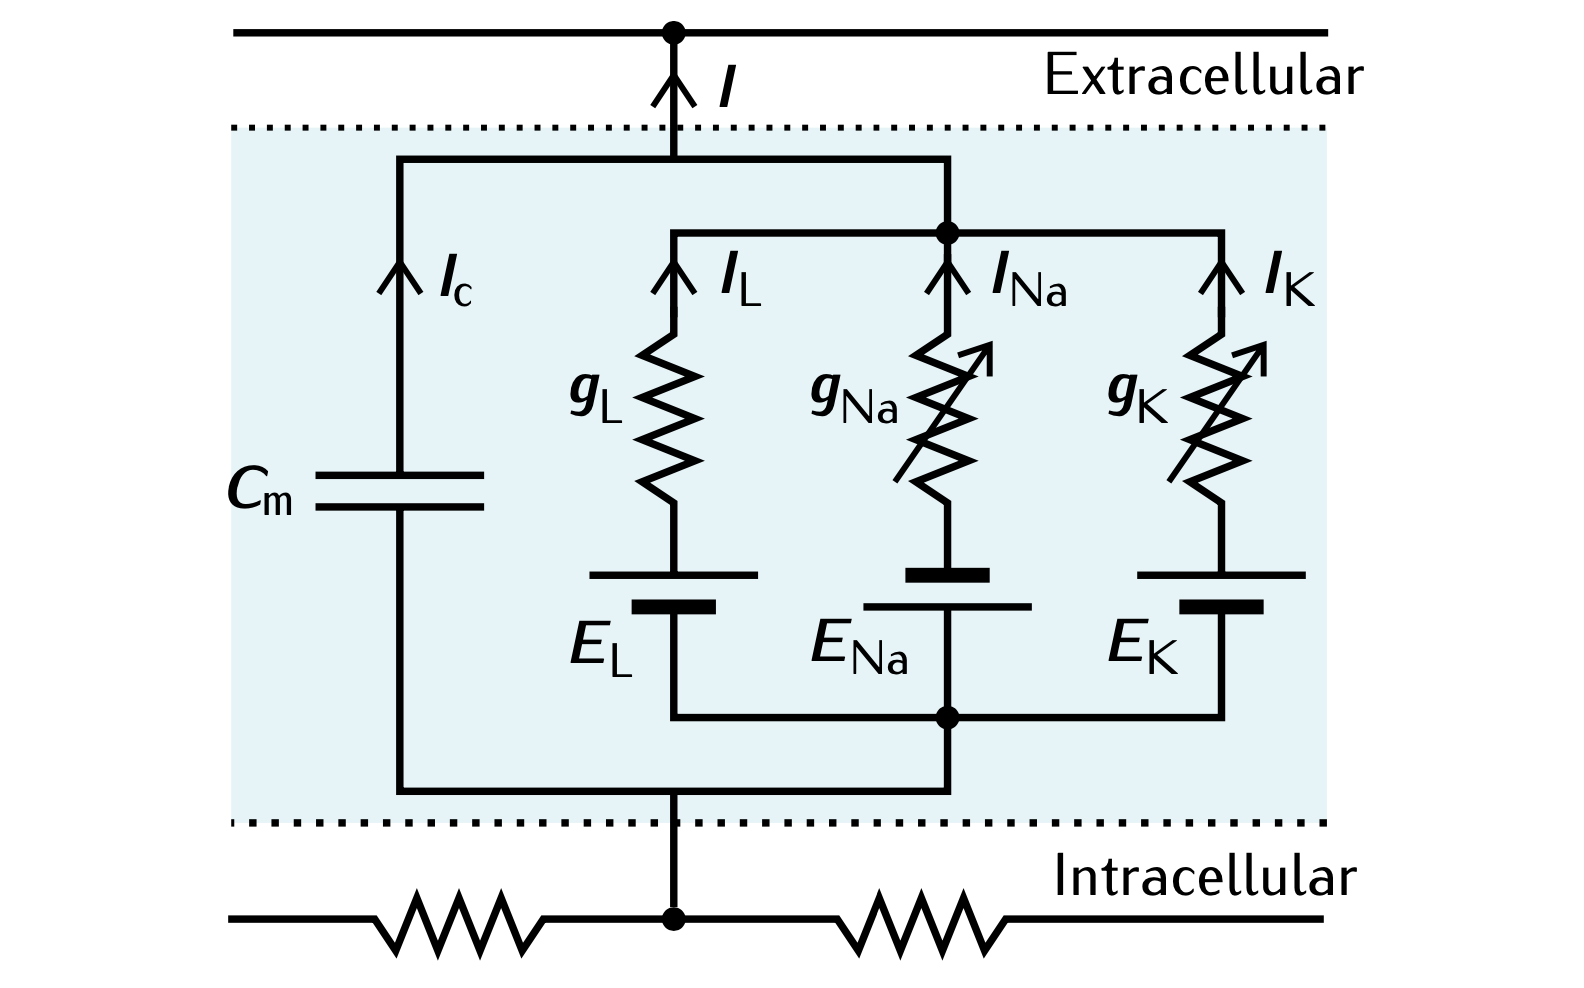
\includegraphics[scale=0.35]{hh_circuit}
    \caption{The HH equivalent circuit. 
    }
    \label{fig:hh_circuit}
    \source{\cite{Sterratt}.}
\end{figure}

Thus, the fundamental total current equation is:
\begin{equation}\label{eq:hh_total_current}
    \begin{aligned}
    I &= I_\mathrm{C} + I_\mathrm{K} + I_\mathrm{Na} + I_\mathrm{L} 
    \\
    &= C_m \frac{\dd{V}}{\dd{t}} + g_\mathrm{K} \qty(V - E_\mathrm{K}) + g_\mathrm{Na} \qty(V - E_\mathrm{Na}) + g_\mathrm{L} \qty(V - E_\mathrm{L})
    \end{aligned}
\end{equation}

In voltage-gated ion channels, the channel conductance $g_\mathrm{X}$ is a function of both voltage and time, $g_\mathrm{X} (V, t)$. We can write the time-dependent conductances like: 

\begin{equation*}
    g_\mathrm{X} (V, t) = \bar{g}_\mathrm{X} p_\mathrm{X} (V, t),
\end{equation*}

where $\bar{g}_\mathrm{X}$ is the total conductance when all channels of type $\mathrm{X}$ are fully open, i.e., the \textit{maximum conductance}, and $p_\mathrm{X} (V, t)$ is the fraction of channels of type $\mathrm{X}$ that are open, i.e., the \textit{channel density} (a number between 0 and 1). Hodgkin and Huxley suggested that the opening and closing of the voltage-gated ion channels were controlled by one or more \textit{gating particles}. Using a series of voltage clamp experiments, i.e., where the membrane potential is held at a level determined by the experimenter, and clever ionic substitutions, they were able to isolate the voltage-gated conductances of potassium and sodium. They obtained rate constants for the opening, closing and inactivation of the conductances by analyzing the voltage-dependence using first-order kinetics, and reduced these rate constants to a set of four ordinary differential equations:

\begin{subequations}\label{eq:hh_model}
    \begin{align}
    C_m \frac{\dd{V}}{\dd{t}} &= - \gbarK n^4 \qty(V - E_\mathrm{K}) - \gbarNa m^3h \qty(V - E_\mathrm{Na}) - \bar{g}_\mathrm{L} \qty(V - E_\mathrm{L}) + I
    \label{eq:hh_model_dVdt}
    \\
    \frac{\dd{n}}{\dd{t}} &= \alpha_n (V) (1-n) - \beta_n (V) n 
    \label{eq:hh_model_dndt}
    \\
    \frac{\dd{m}}{\dd{t}} &= \alpha_m (V) (1-m) - \beta_m (V) m
    \label{eq:hh_model_dmdt}
    \\
    \frac{\dd{h}}{\dd{t}} &= \alpha_h (V) (1-h) - \beta_h (V) h
    \label{eq:hh_model_dhdt}
    \end{align}
\end{subequations}

where the gating variables $n$, $m$ and $h$ are dimensionless quantities that are associated with potassium channel activation, sodium channel activation and sodium channel inactivation, respectively. The gating variables $n$ and $m$ range from $0$ (not activated) to $1$ (fully activated) and $h$ ranges from $0$ (fully inactivated) to $1$ (no inactivation). The voltage-dependent rate constants $\alpha_x (V)$ and $\beta_x(V)$, where $x \in \qty{n,m,h}$, represent the activation and inactivation rates, respectively, for gate $x$. \autoref{eq:hh_model} describes how the membrane potential $V$ across a membrane with capacitance $C_m$ responds to an input current $I$. Note that \autoref{eq:hh_model_dVdt} has been slightly reorganized from the formulation of the total current equation (\autoref{eq:hh_total_current}) to better reflect this. The potassium current, $I_\mathrm{K}$, is controlled by four identical gating particles, whereas the sodium current, $I_\mathrm{Na}$, is controlled by three identical and one distinct gating particle. The leak current, $I_\mathrm{L}$, is not voltage-dependent, and no gating particles are therefore associated with its conductance.

The forms of the $\alpha_x$ and $\beta_x$ functions were empirically proposed by the authors to fit the experimental recordings, yielding the following equations for the rate constants associated with the potassium activation gating variable;

\begin{subequations}
    \begin{align}
        \alpha_n (V) &= 0.01 \frac{V + 55}{1 - \exp \qty(-(V+55)/10)}
        \\
        \beta_n (V) &= 0.125 \exp \qty(-(V+55)/10)
    \end{align}
\end{subequations}

and for the sodium activation and inactivation gating variables: 

\begin{subequations}
    \begin{align}
        \alpha_m (V) &= 0.1 \frac{V + 40}{1 - \exp \qty(-(V+40)/10)}
        \\
        \beta_m (V) &= 4 \exp \qty(-(V+65)/18)
        \\
        \alpha_h (V) &= 0.07 \exp \qty(-(V+65)/20)
        \\
        \beta_h (V) &= \frac{1}{\exp \qty(-(V+35)/10) + 1}
    \end{align}
\end{subequations}


Here, we use a formulation of the model where the membrane voltage has been reversed in polarity from the original HH convention and shifted to reflect a resting potential of $-65 \mV$. An example of how to arrive at the alternative formulation is provided in \autoref{sec:Appendix B}. The original model parameter values are summarized in \autoref{tab:hh_model_parameters}.

\begin{table}[!htb]
  \caption{The original parametrization of the HH model.}
  %\footnotesize%
  \begin{center}
    \rowcolors{2}{gray!15}{white}
    \begin{tabular}{lll}
      \toprule
      \textbf{Parameter} & \textbf{Value} & \textbf{Description} \\
      \midrule
      $C_m$ & $1.0 \, \mathrm{\mu F \, cm}^{-2}$ & Membrane capacitance
      \\
      $\gbarK$ & $36.0 \gunit$ & Maximum potassium channel conductance 
      \\
      $\gbarNa$ & $120.0 \gunit$ & Maximum sodium channel conductance 
      \\
      $\bar{g}_\mathrm{L}$ & $0.3 \gunit$ & Maximum leakage channel conductance
      \\
      $E_\mathrm{K}$ & $-77.0 \mV$ & Potassium reversal potential
      \\
      $E_\mathrm{Na}$ & $50.0 \mV$ & Sodium reversal potential
      \\
      $E_\mathrm{L}$ & $-54.4 \mV$ & Leak reversal potential
      \\
      \bottomrule
    \end{tabular}
  \end{center}
  \label{tab:hh_model_parameters}
\end{table}

%================================================================ 
\subsection{Simulation of Action Potentials}
%================================================================ 

\autoref{fig:hh_states} shows the numerical solutions of a simulation of the HH model. As seen in the top panel, the shape of the simulated action potentials match the description of an action potential (see \cref{sec:ion_ch_and_ap}) well. Besides reproducing action potentials, the HH model offers insights into the mechanisms underlying them. The middle panel shows how the gating variables change during the temporal evolution of the action potentials. At stimulus onset (starting at $t=10 \ms$), the initial depolarization of the membrane potential is due to the input current. When the depolarization is above the threshold (at about $-55 \mV$), the sodium current activates, as reflected in the increase in $m$. As the sodium reversal potential is far higher than the resting membrane potential, the driving force of the sodium current pushes the membrane potential to sharply increase. The slower potassium conductance, reflected by the gating variable $n$, activates after the sharp rise in membrane potential and allows potassium ions to flow out of the neuron because of the low potassium reversal potential. In addition, the repolarization of the membrane potential is also assisted by the inactivating sodium gating variable, $h$, which shuts off the sodium current. This drives the membrane potential quickly back down towards its resting state, but undershoots somewhat, due to the slow de-inactivation of the sodium current, to hyperpolarize the neuron. The final recovery involves a rapid deactivation of the sodium current and a slower deactivation of the potassium current. Eventually all the state variables and the membrane potential return to their resting states. The HH model also explains the refractory period. Relative to the duration of an action potential, the gating variables recover to their resting states slowly. During this period, it is harder to generate an action potential. In the initial recovery phase, an increasing voltage will not increase the sodium conductance, and hence the membrane potential, considerably due to the ongoing inactivation of the sodium current and the prolonged activation of the potassium current. As the state variables advances in their recovery toward the resting states, an action potential can be initiated but will have a lower peak voltage. 

\begin{figure}[H]
    \centering
    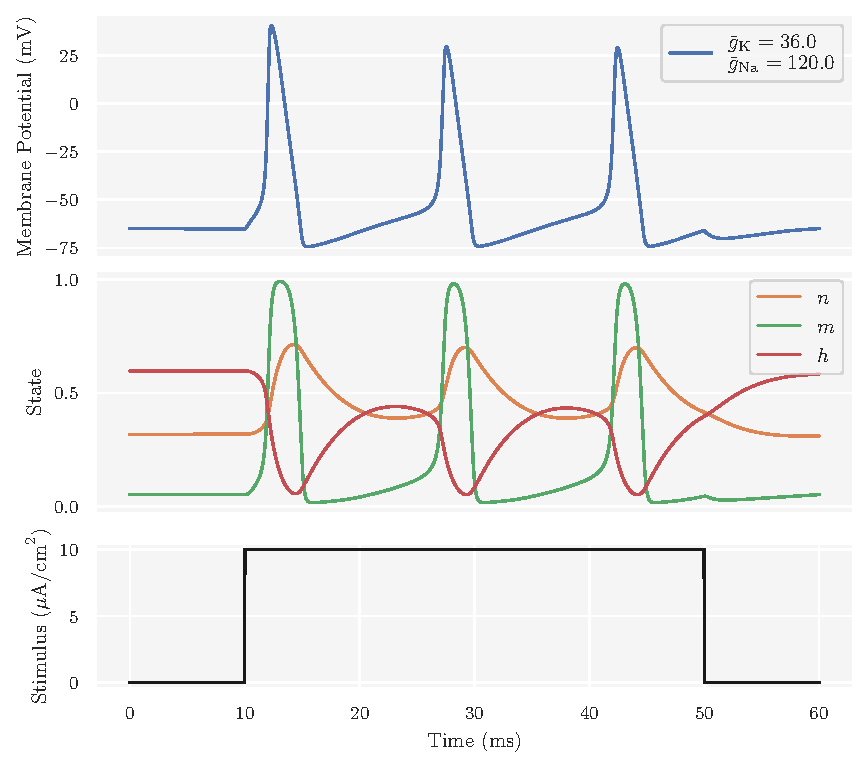
\includegraphics[scale=1.0]{hh_states}
    \caption{Simulated dynamics of $V$, $n$, $m$ and $h$ in the HH model during the firing of action potentials in the squid giant axon. The top panel shows the numerical solution of \autoref{eq:hh_model_dVdt} and the middle panel the numerical solutions of \Crefrange{eq:hh_model_dndt}{eq:hh_model_dhdt}. The system is simulated for $T = 60 \ms$ with time resolution $\Delta t=0.025 \ms$. The input stimulus received by the neuron (bottom panel) is a step current with amplitude $I = 10 \, \mathrm{\mu A/cm}^2$, and onset and offset at $10 \ms$ and $50 \ms$, respectively. The parametrization of the model is given by \autoref{tab:hh_model_parameters}. 
    }
    \label{fig:hh_states}
\end{figure}





%================================================================ 
%================================================================ 
%================================================================ 
%================================================================ 
%================================================================ 



%================================================================
\section{The Brunel Network Model}\label{sec:brunel_model}
%================================================================

Many neural networks of interest consist of thousands or millions of neurons, and, generally, it is infeasible to include all in the model. Neural network models are usually scaled down according to the ratio of different neuron populations in the network that the model tries to mimic. Furthermore, they often use simplified neuron models to reduce computational cost. Still, neural network models may exhibit a high diversity of spiking dynamics. In this section, we present one such model that is thoroughly analyzed in the literature; the Brunel network model \cite{Brunel2000}. Before we present the network model itself, we first discuss the central building block of the network: the leaky integrate-and-fire (LIF) neuron model. 


%================================================================
\subsection{Integrate-And-Fire Neurons}
%================================================================

While the ionic mechanisms behind APs are quite complicated, the conditions for AP generation are often quite straightforward: When the membrane potential reaches a specific threshold, a spike is generated and the membrane potential returns to the background state. Simulations of APs can be accelerated significantly by not explicitly modeling the responsible biophysical mechanisms. \textit{Integrate-and-fire} (IF) models are simplified neuron models with a spike generation and reset mechanism. In these models, whenever the membrane potential of a neuron reaches a threshold value $\theta$, a spike is generated and the membrane potential is reset to a value $V_\mathrm{reset}$ below the threshold potential, $V_\mathrm{reset} < \theta$. In the simplest IF model, all active membrane conductances are ignored and the entire membrane conductance is modeled as a single passive leakage conductance: 

\begin{equation*}
    I_\mathrm{L} = \bar{g}_\mathrm{L} \qty(V - E_m),
\end{equation*}

where $E_m$ is the resting membrane potential. Since the conductance is the reciprocal of the resistance, the above equation can be equivalently formulated as: 

\begin{equation*}
    I_\mathrm{L} = \frac{V - E_m}{R_m},
\end{equation*}

where $R_m$ is the membrane resistance. Furthermore, we assume that the model neuron behaves like an electric circuit consisting of a resistor and a capacitor in parallel, i.e., an RC circuit, driven by a current $I$. In addition, the circuit needs a switch, representing the reset mechanism, which is open until the membrane potential reaches $\theta$ and then closes to short-circuit the membrane resistance, bringing the membrane potential back to rest. The switch opens again after a refractory period $\tau_\mathrm{rp}$, allowing the membrane to charge. This neuron model is often called the \textit{leaky integrate-and-fire} (LIF) model. The circuit diagram and the RC circuit response to input stimulus is shown in \autoref{fig:lif_circuit}. When the membrane potential is below the threshold, its value is determined by the equation for an RC circuit: 

\begin{figure}[!htb]
    \centering
    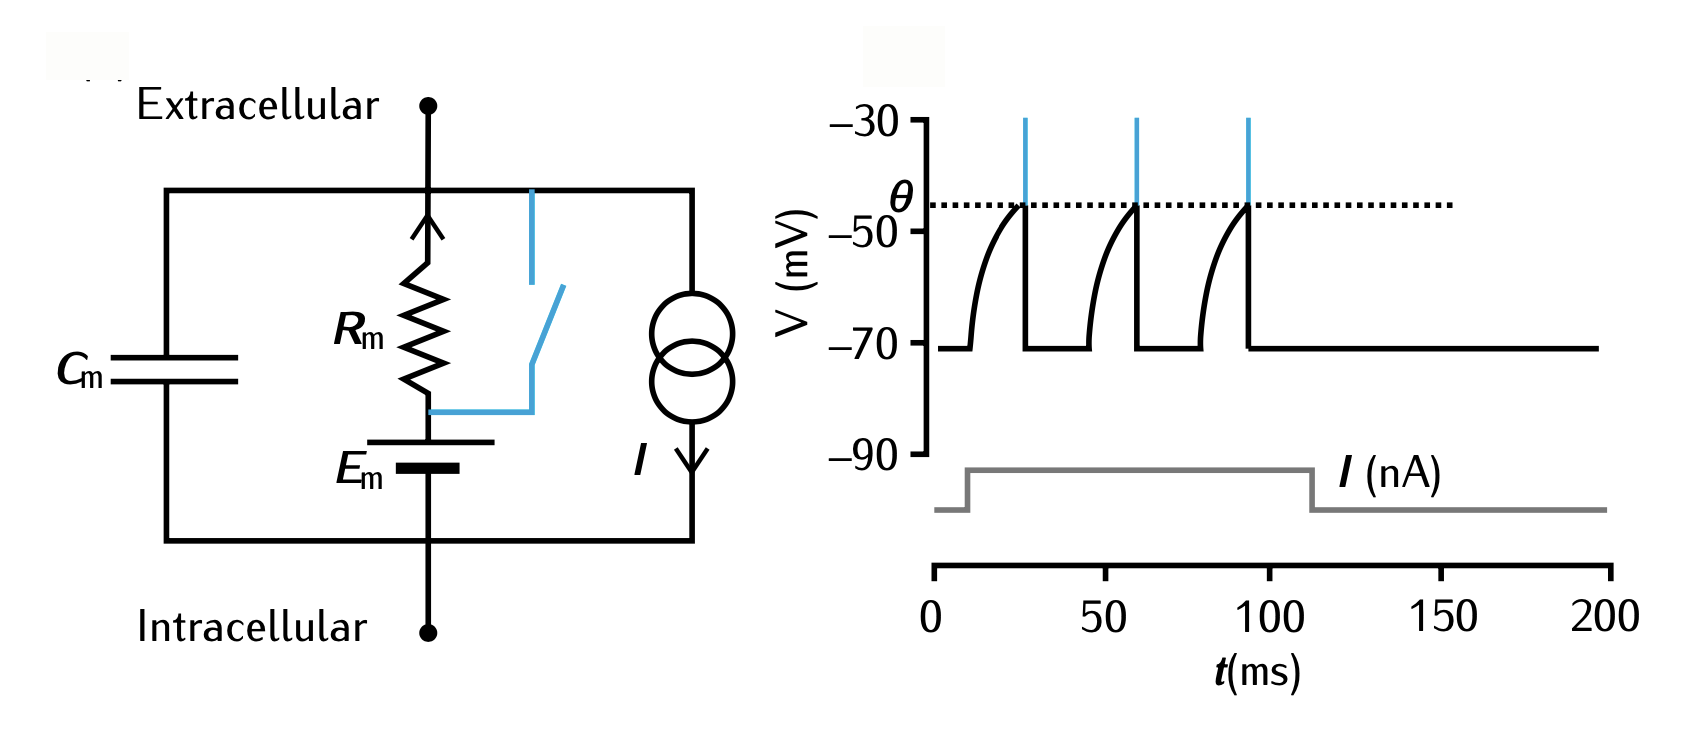
\includegraphics[scale=0.45]{lif_circuit}
    \caption{The LIF neuron model as an RC circuit diagram (left) with a switch (in blue on the diagram) and the response of the LIF neuron to input stimulus (right). When the switch is open, the membrane can charge. When the membrane potential reaches the threshold $\theta$ (indicated by the dashed line in the voltage trace), the neuron fires a spike (indicated by the vertical blue line in the voltage trace) and the switch closes. This short-circuits the membrane resistance, bringing the membrane potential back to its resting state. After a refractory period, the switch opens, allowing the membrane to charge again.
    }
    \label{fig:lif_circuit}
    \source{\cite{Sterratt}.}
\end{figure}

\begin{equation*}
    C_m \frac{\dd{V}}{\dd{t}} = - \frac{V-E_m}{R_m} + I.
\end{equation*}

The above equation is usually written in terms of the membrane time constant, $\tau_m = C_m R_m$: 

\begin{equation*}
    \tau_m \frac{\dd{V}}{\dd{t}} = - V + E_m + R_m + I.
\end{equation*}

Furthermore, the leak battery is often omitted from the circuit, with the only effect of making the resting membrane potential $0\mV$ instead of $E_m$: 

\begin{equation}\label{eq:lif_model}
    \tau_m \frac{\dd{V}}{\dd{t}} = - V + R_m + I.
\end{equation}

The simple LIF neuron model only captures the timing of each spike, but is fast to simulate compared to biophysically detailed neuron models. This makes it especially useful for simulating large networks, as these often contain thousands of neurons. 



%================================================================
\subsection{A Sparsely Connected Recurrent Network}\label{sec:recurrent_network}
%================================================================

The local cortical network consists of a population of excitatory neurons and a population of inhibitory neurons, with a ratio of about $80\%$ excitation and $20\%$ inhibition. The Brunel model characterizes the local cortical network as a network of $N$ identical LIF neurons, from which $N_E$ are excitatory and $N_I = N_E / 4$ inhibitory. Each neuron, be it excitatory or inhibitory, receives $C$ randomly connections from other neurons in the network, from which $C_E = \epsilon N_E$ are from the excitatory population and $C_I = \epsilon N_I$ from the inhibitory population. Here, $\epsilon$ denotes the fraction of incoming connections, and we consider a sparsely connected network with $\epsilon = C_E / N_E = C_I / N_I << 1$. In addition to the sparse recurrent inputs from within the local network, each neuron receives excitatory synaptic input from a population of $C_E$ randomly firing neurons outside the network with activation governed by identical, independent Poisson processes (PGs) with fixed-rate $\nu_\mathrm{ext}$. The randomly firing population mimics input from the rest of cortex. An illustration of the network is shown in \autoref{fig:brunel_diagram}.

\begin{figure}[!htb]
    \centering
    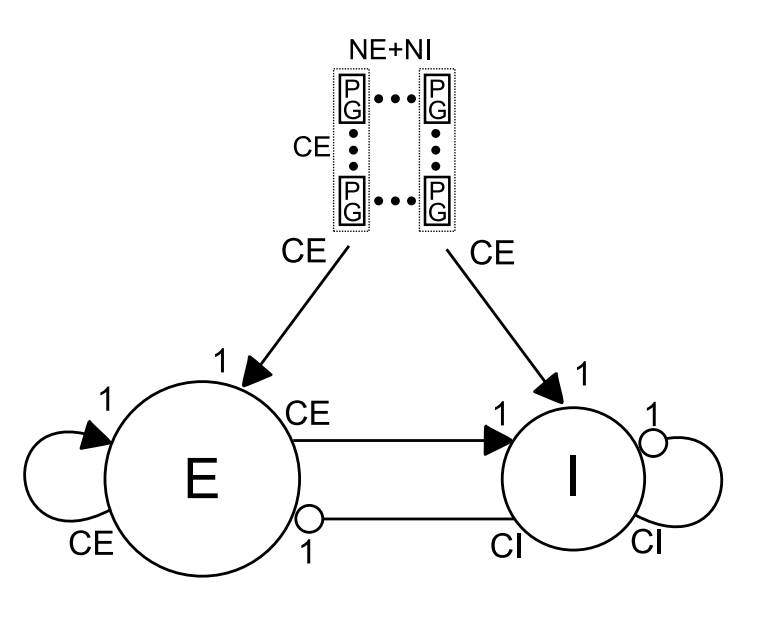
\includegraphics[scale=0.5]{brunel_diagram}
    \caption{Illustration of the Brunel network model. The network consists of two local populations, one with $N_E$ excitatory neurons (circle labeled E) and one with $N_I$ inhibitory neurons (circle labeled I), and one external population of identical, independent Poisson processes (PGs). The connections between network nodes are indicated by arrows, where triangular arrow-heads represent excitatory and round arrow-heads inhibitory connections. The numbers at the start and end of each arrow indicate the multiplicity of the connection.
    }
    \label{fig:brunel_diagram}
    \source{\cite{nest_by_example}.}
\end{figure}

The subthreshold dynamics of LIF neuron $i$ in the network ($i=1, ..., N$) evolves in time according to:

\begin{equation}
    \tau_m \frac{\dd{V_i (t)}}{\dd{t}} = - V_i(t) + R_m I_i(t),
\end{equation}

where $I_i$ are the synaptic inputs arriving at the soma. These synaptic inputs are the sum of spike contributions from both local and external synapses, and are modeled as $\delta$-current inputs, i.e., discontinuous voltage jumps: 

\begin{equation}
    R_m I_i (t) = \tau_m \sum_j J_{ij} \sum_k \delta \qty(t - t_j^k - D),
\end{equation}

where the first sum is over all the presynaptic neurons $j$ with postsynaptic potential amplitude (voltage jump) $J_{ij}$, while the second sum is over the spike times of those neurons. Here, $D$ is the synaptic delay, $\delta(x)$ the Dirac $\delta$ function, with $\delta(x)=0$ for $x \neq 0$ and $\int_{-\infty}^\infty \delta (x) \dd{x} = 1$, and $t_j^k$ represents the emission time of the $k$th spike of presynaptic neuron $j$. For simplicity, we assume the synaptic connection strengths are constant for each population. We let $J_{ij}=J>0$, and for excitatory neurons and external input $J_E = J$, while for inhibitory neurons $J_I = -g J_E$, where $g$ determines the relative strength of the inhibitory synapses compared to the excitatory synapses. The amount of input the local neurons receive from the external population is determined by the parameter $\eta = \nu_\mathrm{ext}/\nu_\mathrm{thr}$, where $\nu_\mathrm{thr} = \theta / \qty(J_E C_E \tau_m)$ is the minimum constant rate input needed for a neuron to reach threshold in absence of feedback. Thus, the external input rate is given by $\nu_\mathrm{ext} = \qty(\eta \theta) / \qty(J_E C_E \tau_m)$.  

When the membrane potential $V_i (t)$ of LIF neuron $i$ reaches the firing threshold $\theta$, the neuron fires a spike, the synapses onto all its postsynaptic neurons are activated after a time delay $D$ and the neuron's membrane potential is clamped to the reset potential $V_\mathrm{reset}$ for a refractory period $\tau_\mathrm{rp}$.


%================================================================
\subsection{States of Spiking Activity}
%================================================================

The Brunel network may be in several different states of spiking activity, largely dependent on the values of the synaptic weight parameters. In the context of a biological neural network, synaptic weight parameters refer to parameters that determines the influence the firing of one neuron has on another. With particular fixed values for $J$ and $D$ and varying values for $\eta$ and $g$, Brunel \cite{Brunel2000} characterized the spiking activity of the network by phase diagrams. An example of these is shown in \autoref{fig:brunel_phase}. The spiking activity can be in a state of synchronous regular (SR), asynchronous irregular (AI) or synchronous irregular (SI), with either fast or slow oscillations, activity. It can be seen from the phase diagram that $g=4$ corresponds to balance between excitation and inhibition, while $\eta=1$ corresponds to external input, in the absence of recurrent input from the network, just sufficient to reach the firing threshold. Stability of the AI state breaks down at the dashed or solid lines and can lead to SR or SI (either fast or slow) activity.

\begin{figure}[!htb]
    \centering
    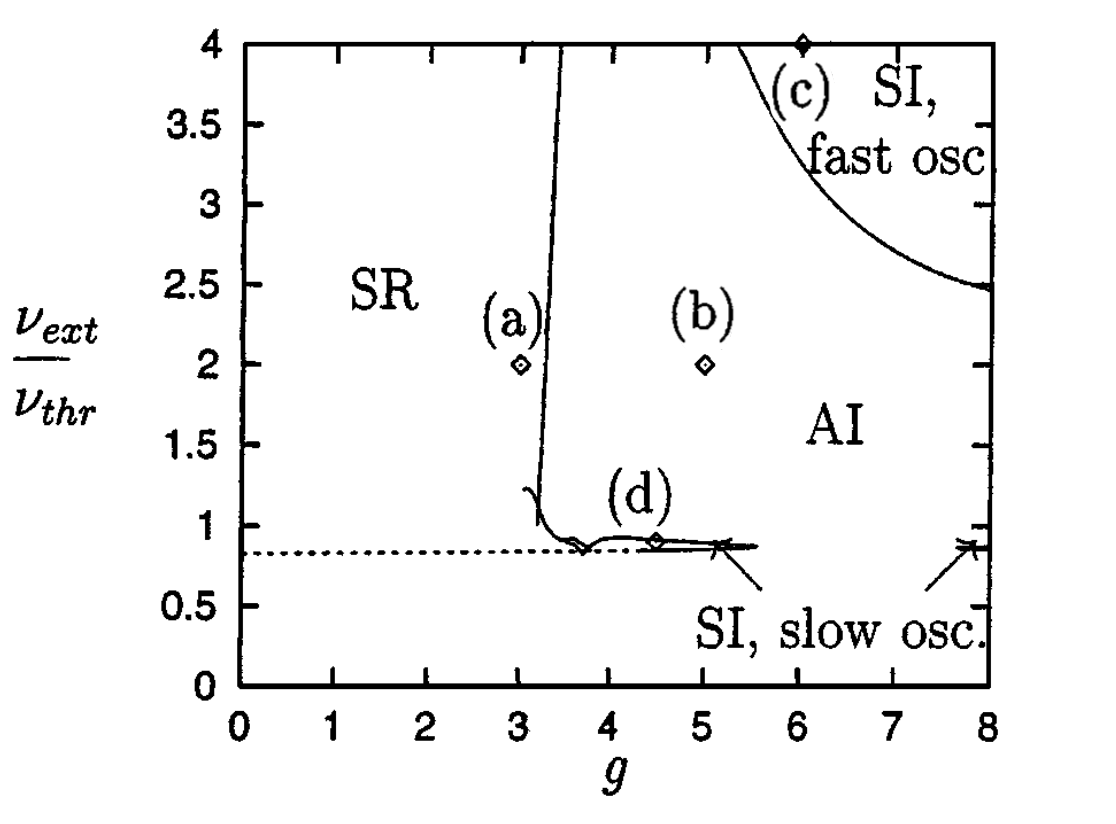
\includegraphics[scale=0.45]{brunel_phase}
    \caption{Phase diagram of different network states which arise depending on the parameters $\eta = \nu_\mathrm{ext}/\nu_\mathrm{thr}$ and $g$. In the present example, a fixed synaptic delay $D=1.5\ms$ and voltage jump (amplitude of excitatory synaptic input currents)  $J_E = 0.1 \mV$ is used. The simulation is of a network consisting of $N_\mathrm{E}=10,000$ excitatory and $N_\mathrm{I} = 2,500$ inhibitory neurons with connection probability $\epsilon = 0.1$, which corresponds to a network where each neuron has $C_\mathrm{E}=1,000$ and $C_\mathrm{I}=250$ randomly selected connections to excitatory and inhibitory neurons, respectively. The phase diagram shows four states of spiking activity: synchronous regular (SR), asynchronous irregular (AI) and of synchronous irregular (SI), fast and slow. The four points (shown by diamonds) indicate the example activities shown in \autoref{fig:brunel_states}.
    }
    \label{fig:brunel_phase}
    \source{\cite{Brunel2000}.}
\end{figure}

\autoref{fig:brunel_states} illustrates an example of each of the states of the Brunel network. For each state, the figure shows the firing times (rasters) of 20 randomly chosen excitatory neurons, the temporal evolution of the activity in the network (time resolved firing rate computed in bins of 10 ms) together with the mean firing rate (horizontal axis line), and the pairwise Pearson's correlation coefficient matrix (described in the next chapter) of the recorded neurons. The particular values for $\eta$ and $g$ are stated in the subplot titles and correspond to the points (diamonds) in \autoref{fig:brunel_phase}. In the SR state, the network is almost fully synchronized and the neurons fire at high rates. It is characterized by fast periodic oscillations of the spiking activity. In the AI state, neurons fire mostly independently at low rates. It is characterized by that neurons in the population fire at different times (\textit{asynchronous firing}) and at irregular intervals. In the SI states, the spiking activity of the network is characterized by either fast or slow synchrony, but individual neurons fire irregularly. It can be traced back to an instability of the AI firing regime towards oscillatory activity. The pairwise Pearson's correlation coefficient measures the correlation between spike trains of two neurons in the network, and can be used to examine how synchronous the spiking of a network is. We see that in the SR state, the correlation coefficients are much higher than in the AI state. The SI state with fast oscillations, however, is only scarcely more synchronous than the AI state. The SI state with slow oscillations, on the other hand, has increased synchrony compared to the AI state. 

\begin{figure}[H]
    \centering
    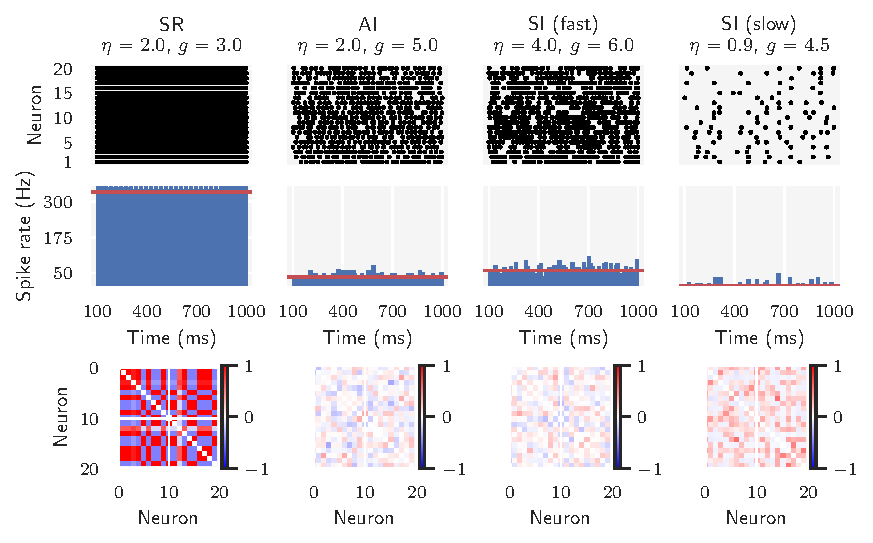
\includegraphics[scale=1.0]{brunel_states}
    \caption{Simulation of the network specified by \autoref{tab:bnet_model_parameters}, with the values of $\eta$ and $g$ stated in each subplot's title along with the network state. The network is simulated for $T_\mathrm{sim} = 1,000$ ms, and we record the output from $N_\mathrm{rec} = 20$ excitatory neurons. To avoid transient effects, we start recording after $T_\mathrm{transient} = 100$ ms. The top row shows the firing times (raster) of the recorded neurons. Each point in the raster corresponds to the firing of a neuron. The second row shows the network activity as a time resolved firing rate computed in bins of $10 \ms$. The mean firing rate is indicated by the horizontal (red) axis line. The third row shows the pairwise Pearson's correlation coefficient matrix of the recorded neurons.
    }
    \label{fig:brunel_states}
\end{figure}


\autoref{tab:bnet_model_parameters} summarizes the parametrization of the Brunel model used in the above simulations.

\begin{table}[!htb]
  \caption{The parametrization of the Brunel model. Specific values are not provided for the parameters derived from the varying $\eta$ and $g$.}
  %\footnotesize%
  \begin{center}
    \rowcolors{2}{gray!15}{white}
    \begin{tabular}{lll}
      \toprule
      \textbf{Parameter} & \textbf{Value} & \textbf{Description} \\
      \midrule
      $N$ & $12,500$ & Total number of neurons
      \\
      $N_E$ & $10,000$ & Number of excitatory neurons
      \\
      $N_I$ & $2,500$ & Number of inhibitory neurons
      \\
      $\epsilon$ & $0.1$ & Connection probability
      \\
      $C_E$ & $1,000$ & Excitatory synapses per neuron
      \\
      $C_I$ & $200$ & Inhibitory synapses per neuron
      \\
      $E_m$ &  $0 \mV$ & Resting membrane potential 
      \\
      $C_m$ &  $1 \, \mathrm{pF}$ & Membrane capacitance
      \\
      $\tau_m$ &  $20 \ms$ & Membrane time constant
      \\
      $\theta$ &  $20 \mV$ & Firing threshold
      \\
      $V_\mathrm{reset}$ &  $10 \mV$ & Reset membrane potential
      \\
      $\tau_\mathrm{rp}$ &  $2 \ms$ & Refractory period
      \\
      $D$ &  $1.5 \ms$ & Synaptic delay
      \\
      $J_E$ &  $0.1 \mV$ & Excitatory synapse strength
      \\
      $J_I$ &  $-g J_E$ & Inhibitory synapse strength
      \\
      $\nu_\mathrm{ext}$ &  $\qty(\eta \theta)/\qty(J_E C_E \tau_m)$ & External firing rate
      \\
      \bottomrule
    \end{tabular}
  \end{center}
  \label{tab:bnet_model_parameters}
\end{table}
 
%-------------------- examples -----------------------
%================================================================
\chapter{Theoretical Background}
%================================================================

%================================================================
\section{Theory}\label{sec:Theory}
%================================================================

%----------------------------------------------------------------
\subsection{Project Theory 1}\label{sec:project theory}
%----------------------------------------------------------------
This is \autoref{sec:project theory}.

Citation is done with \hologo{BibTeX} \cite[p.~100]{Sakurai}.

Cross-reference equations such as
\begin{equation}\label{eq:einstein}
    E = m c^2
\end{equation}
with \cref{eq:einstein}.

\autoref{fig:noise} brings the noise from the \textbf{figures folder}. 
\begin{figure}[H]
\begin{center}
\includegraphics[scale=0.5]{example} 
\end{center}
\caption{Make some noise.}
\label{fig:noise}
\end{figure}

\autoref{fig:happy} shows a happy animal found in the \textbf{Images folder}. 
\begin{figure}[H]
\begin{center}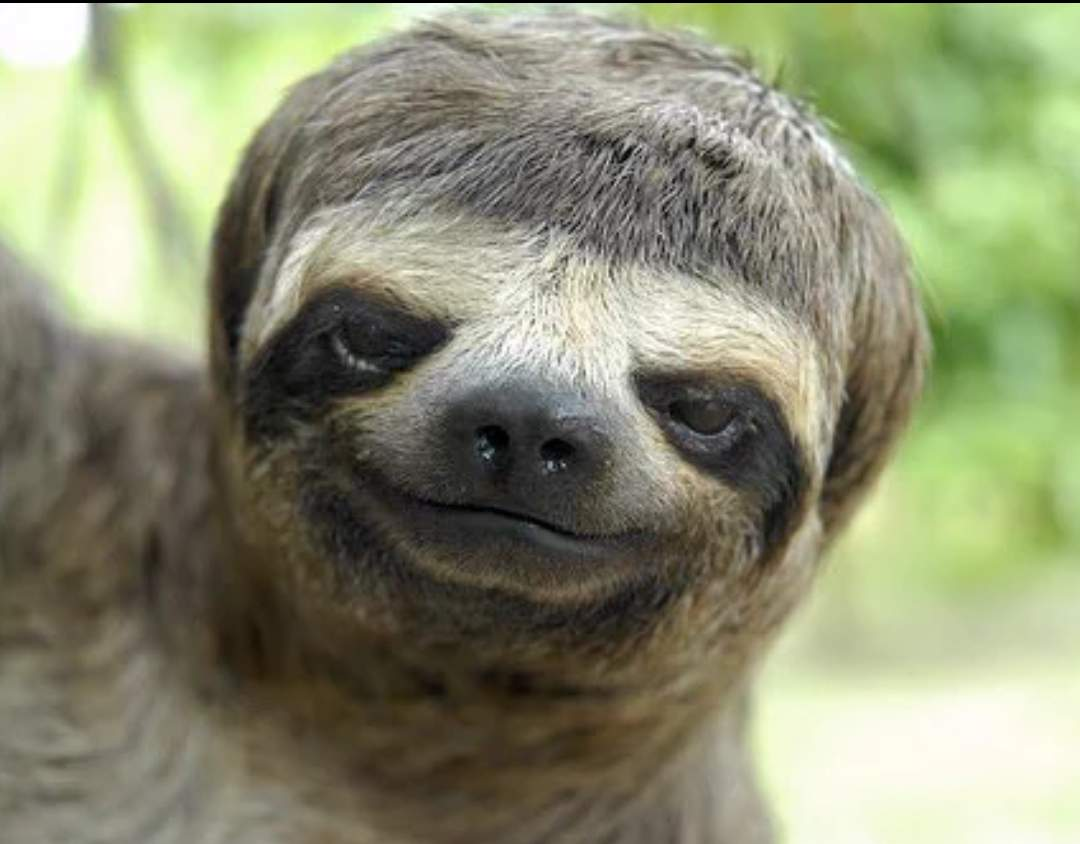
\includegraphics[scale=0.5]{./3_Images/Funny-Animal-Face} 
\end{center}
\caption{Sloths are arboreal mammals noted for slowness of movement and for spending most of their lives hanging upside down in the trees.}
\label{fig:happy}
\source{Insert image source here}
\end{figure}

The Hodgkin–Huxley model, or conductance-based model, is a mathematical model that describes how action potentials in neurons are initiated and propagated. It is a set of nonlinear differential equations that approximates the electrical characteristics of excitable cells such as neurons and cardiac myocytes. It is a continuous-time dynamical system.


\begin{figure}[hbt!]
    \centering
    \begin{subfigure}[c]{.45\linewidth}
        
\includegraphics[scale=0.5]{example} 
        \caption{Sloth A}
    \end{subfigure}
    \begin{subfigure}[c]{.45\linewidth}
        
\includegraphics[scale=0.5]{example} 
        \caption{}
    \end{subfigure}
    \caption{Sloths are arboreal mammals noted for slowness of movement and for spending most of their lives hanging upside down in the trees.}
    \label{fig:my_label}
\end{figure}


The Hodgkin–Huxley model, or conductance-based model, is a mathematical model that describes how action potentials in neurons are initiated and propagated. It is a set of nonlinear differential equations that approximates the electrical characteristics of excitable cells such as neurons and cardiac myocytes. It is a continuous-time dynamical system.

\begin{figure}[H]
\centering
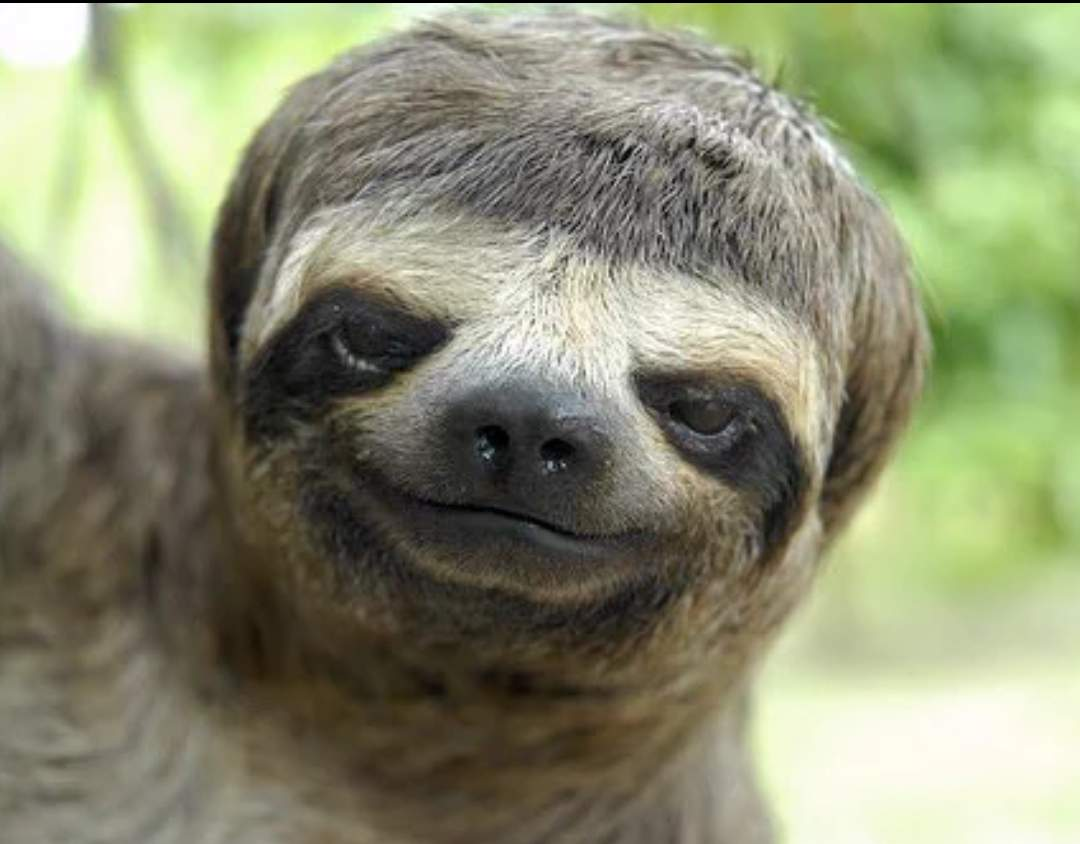
\includegraphics[width=0.5\textwidth]{./3_Images/Funny-Animal-Face} 
\caption{Sloths are arboreal mammals noted for slowness of movement and for spending most of their lives hanging upside down in the trees.}
\label{fig:happy2}
\source{Insert image source here}
\end{figure}




\autoref{tab:tab1} is from the \textbf{tables folder}. 
\begin{table}[H]
\caption{From pandas to latex.}
\centering
\rowcolors{2}{gray!25}{white}
\begin{tabular}{ccc}
\hline \hline
  $x$ &  $x^2$ &  $x^3$ \\
\hline \hline
0.250 &  0.062 &  0.016 \\
0.500 &  0.250 &  0.125 \\
0.750 &  0.562 &  0.422 \\
\hline \hline
\end{tabular}

\label{tab:tab1}
\end{table}

\autoref{tab:alternate} tabulates some values with alternating row colors.
\begin{table}[H]
\caption{Alternating background color for rows.}
\centering
\rowcolors{2}{gray!25}{white}
\begin{tabular}{ccc}
\hline
\hline 
$\alpha$ & $\beta$ & $\gamma$
\\
\hline 
\hline 
0.1 & 0.2 & 0.3
\\
0.4 & 0.5 & 0.6
\\
0.7 & 0.8 & 0.9
\\
\hline
\hline 
\end{tabular}
\label{tab:alternate}
\end{table} 

Table with nice rulers 

\begin{table}[h]
  \caption{Generic table with different sized rulers.}
  \footnotesize%
  \begin{center}
    \begin{tabular}{cccc}
      \toprule
      header1 & header2 & header3 & header4 \\
      \midrule
      col1 &  col2 & col3 & col4 \\
      col1 &  col2 & col3 & col4 \\
      col1 &  col2 & col3 & col4 \\
      col1 &  col2 & col3 & col4 \\
      \bottomrule
    \end{tabular}
  \end{center}
  \label{tab:tablerule}
\end{table}

Table with nice rulers and alternating rows

\begin{table}[h]
  \caption{Generic table with alternating rows and different sized rulers.}
  \footnotesize%
  \begin{center}
    \rowcolors{2}{white}{gray!15}
    \begin{tabular}{cccc}
      \toprule
      header1 & header2 & header3 & header4 \\
      \midrule
      col1 &  col2 & col3 & col4 \\
      col1 &  col2 & col3 & col4 \\
      col1 &  col2 & col3 & col4 \\
      col1 &  col2 & col3 & col4 \\
      \bottomrule
    \end{tabular}
  \end{center}
  \label{tab:tablerule2}
\end{table}

Table with nice rulers and alternating rows 2

\begin{table}[h]
  \caption{Generic table with alternating rows and different sized rulers.}
  \footnotesize%
  \begin{center}
    \rowcolors{2}{gray!15}{white}
    \begin{tabular}{cccc}
      \toprule
      header1 & header2 & header3 & header4 \\
      \midrule
      col1 &  col2 & col3 & col4 \\
      col1 &  col2 & col3 & col4 \\
      col1 &  col2 & col3 & col4 \\
      col1 &  col2 & col3 & col4 \\
      \bottomrule
    \end{tabular}
  \end{center}
  \label{tab:tablerule3}
\end{table}

Given
\begin{align*}
    f\colon \R \to \R,
    \intertext{magic happens}
    \int_{0}^{\infty} \mathrm{e}^{-x}\,\mathrm{d}x
\end{align*}


This is
\todo[inline]{Rewrite this!}

\section{Figures and Tables}

% Todonotes:
\begin{figure}[hbp]
    \centering
    \missingfigure{Three balls.}
    \caption[Three balls]{Three balls.}
\end{figure}


% Booktabs:
\begin{table}[htbp]
    \centering
    \begin{tabular}{@{}ll@{}}
        \toprule
        \textbf{Correct}               & \textbf{Incorrect}      \\
        \midrule
        \( \varphi \colon X \to Y \)   & \( \varphi : X \to Y \) \\[0.5ex]
        \( \varphi(x) \coloneqq x^2 \) & \( \varphi(x) := x^2 \) \\
        \bottomrule
    \end{tabular}
    \caption[Colons]{Proper colon usage.}
\end{table}

\begin{table}[htbp]
    \centering
    \begin{tabular}{@{}ll@{}}
        \toprule
        \textbf{Correct}     & \textbf{Incorrect}         \\
        \midrule
        \( A \implies B \)   & \( A \Rightarrow B \)      \\
        \( A \impliedby B \) & \( A \Leftarrow B \)       \\
        \( A \iff B \)       & \( A \Leftrightarrow B \)  \\
        \bottomrule
    \end{tabular}
    \caption[Arrows]{Proper arrow usage.}
\end{table}

% Tablefootnote and multirow:
\begin{table}[htbp]
    \centering
    \begin{tabular}{@{}ll@{}}
        \toprule
        \textbf{Correct}
        & 
        \textbf{Incorrect}
        \\
        \midrule
        \( -1 \) 
        & 
        -1
        \\[0.3ex]
        1--10
        &
        1-10
        \\[0.3ex]
        Birch--Swinnerton-Dyer conjecture
        &
        Birch-Swinnerton-Dyer conjecture
        \\[0.3ex]
        The ball \dash which is blue \dash is round.
        &
        \multirow{ 2}{*}{The ball - which is blue - is round.}
        \\[0.3ex]
        The ball---which is blue---is round. 
        &
        \\
        \bottomrule
    \end{tabular}
    \caption[Dashes]{Proper dash usage.}
\end{table}

It is now easy to tell that Birch and Swinnerton-Dyer are two people.

\begin{table}[hbtp]
    \centering
    \begin{tabular}{@{}*{2}{p{0.5\textwidth}}@{}}
        \toprule
        \textbf{Correct} &  \textbf{Incorrect}
        \\
        \midrule
        \enquote{This is an \enquote{inner quote} inside an outer quote}
        &
        "This is an 'inner quote' inside an outer quote"
        \\
        \bottomrule
    \end{tabular}
    \caption[Quotation marks]
    {Proper quotation mark usage.
    The \texttt{\textbackslash enquote} command chooses the correct
    quotation marks for the specified language.}
\end{table} 


%==========================================================
%------- part 2: methodology & computational approach -----
%==========================================================
\part{Methodology \& Computational Approach}
%-------------------- placeholder --------------------
%================================================================
\chapter{Methodology}\label{chap:methodology}
%================================================================

%================================================================
\section{Computation}
%================================================================

\subsection{Log densities}

To avoid computational overflows and underflows, one should compute with the logarithm of posterior densities whenever possible. Exponentiation should be performed only when necessary and as late as possible; for example, in the Metropolis algorithm, the required ratio of two densities (11.1) should be computed as the exponential of the difference of the log-densities \cite[p. 261]{BDA}

\subsection{Numerical integration} 


\subsection{MCMC-ABC}

Flip-ordering, accept prob first then simulation

MCMC-ABC was also implemented in pyLFI, however, in order to focus the study on the objective, it is not included in the following analyses as it would not give any significant insights into the questions we seek than the more naive rejection sampler would. 


\subsection{Distance function}

\textbf{Relevant papers:}

* H. Jung and P. Marjoram (2011). "Choice of Summary Statistic Weights in Approximate Bayesian Computation". \url{https://www.ncbi.nlm.nih.gov/pmc/articles/PMC3192002/}
    * Develops a Genetic Algorithm that computes how one should weight the summary statistics 
    * Fairly advanced, so we won't implement their approach, but should be mentioned in thesis
* D. Prangle (2015). "Adapting the ABC distance function". \url{https://arxiv.org/pdf/1507.00874.pdf}
    * Methods for adaptive distances
    * Won't implement this either, but will use the weighted distance defined in the paper
* S. Druckmann et al. (2007) "A novel multiple objective optimization framework for constraining conductance-based neuron models by experimental data". 
    * MOO
    
    
In the ABC algorithms, each simulation is converted to a vector of summary statistics $\mathbf{s} = (s_1, s_2, ..., s_m)$ and a distance between this and the summary statistics of the observed data, $\mathbf{s}_{obs}$, is calculated. Parameters producing distances below some threshold are accepted and form a sample from an approximation to the posterior. 

However, without normalization of the summary statistics, we are comparing oranges with apples. The most variable summaries will dominate the distances because of their larger scales. Handling the scales of the summaries ... blabla ... important.  

Normalizing the summaries so that they vary over roughly the same scale can be achieved by using a weighted Euclidean distance: 

$$ d \left(\mathbf{s}, \mathbf{s}_{obs} \right) = \left[ \sum_{i=1}^m \left( \frac{s_i - s_{obs, i}}{\sigma_i} \right)^2 \right]^{1/2},$$

where $\sigma_i$ is an estimate of the prior predictive standard deviation of the $i$th summary statistic. A convenient estimate is the empirical standard deviation of simulated $s_i$ values. The normalization we acquire from scaling by $\sigma_i$ prevents the distances from being dominated by the most variable summaries.  

Furthermore, we should also weight the importance of the summary statistics ...

\subsection{Sensitivity analysis} 

pearson correlation coefficient

Use Pearson's Coefficient of Correlation to weight importance of summary statistics.

* This is a simple approach for producing weighted statistics 
    * Method developed by H. Jung and P. Marjoram (2011) is more advanced and likely better
* The correlation coefficient, $r$, relates $Y$ to $X$ 
* The squared correlation coefficient, $r^2$, indicates the proportion of variance in $Y$ that is shared with (or accounted for) by $X$.

**Cons of using Pearson's Coefficient of Correlation:**

* Assumes:
    1. Normality of data (meaning that the data should approximate the normal distribution; most data points should tend to hover close to the mean)
    2. Homoscedasticity (means ‘equal variances’), i.e. a situation in which the variance of the dependent variable is the same for all the data.
    3. Linearity; simply means that the data follows a linear relationship. 
* (2. and 3. can be checked visually by scatter plot)
* Is sensitive to outliers; outliers can can significantly skew the correlation coefficient and make it inaccurate. Outliers are also easy to spot visually from the scatter plot

* vekte utifra sensitivitet

\textbf{Relevant papers:}

H. Jung and P. Marjoram (2011). "Choice of Summary Statistic Weights in Approximate Bayesian Computation". \url{https://www.ncbi.nlm.nih.gov/pmc/articles/PMC3192002/}

* Develops a Genetic Algorithm that computes how one should weight the summary statistics 

* Fairly advanced, so we won't implement their approach, but should be mentioned in thesis

\subsection{Summary statistics weights}

\textbf{Relevant papers:}

H. Jung and P. Marjoram (2011). "Choice of Summary Statistic Weights in Approximate Bayesian Computation". \url{https://www.ncbi.nlm.nih.gov/pmc/articles/PMC3192002/}

* Develops a Genetic Algorithm that computes how one should weight the summary statistics 

* Fairly advanced, so we won't implement their approach, but should be mentioned in thesis

* S. Druckmann et al. (2007) "A novel multiple objective optimization framework for constraining conductance-based neuron models by experimental data". 

%================================================================
\section{Notes}
%================================================================

Tabs to open again:

\url{https://learning.oreilly.com/library/view/bayesian-analysis-with/9781789341652/0d1ffa98-7336-4d71-aade-88f0973f4b13.xhtml}

\url{https://arxiv.org/pdf/2012.09612.pdf?fbclid=IwAR1xmEDRcPKHvcHK2KtQ1FO0B8K_yqKRlbPwdYuw0vv3-jjBTTR3CnMQEgY}

\url{https://arxiv.org/pdf/1707.01254.pdf}

\url{https://arxiv.org/pdf/1202.3819.pdf}

\url{https://www.ncbi.nlm.nih.gov/pmc/articles/PMC1462356/pdf/12524368.pdf}

\url{https://github.com/pymc-devs/pymc-examples/blob/main/examples/diagnostics_and_criticism/posterior_predictive.ipynb}

\section{Choice of Priors}

\url{https://en.wikipedia.org/wiki/Prior_probability}


The choice of priors ... beyond the scope of this thesis. We will mainly be using flat (uniform) or informed (normal centered about the true value)

Non- and weakly informative priors, p. 51 and 55 in BDA

As we saw in sec coin flip, the influence of the prior diminishes as more data is available.  


See LFI for cognitive science book, Ch. 2.1

Although the steps listed above may give the impression that all likelihood- free algorithms are simple, this is unfortunately not the case. Many sophisticated techniques have been created in the hopes of increasing the efficiency of an algorithm on a given problem, and as one might expect, the efficiency of the algorithms below do vary by the type of problem to which they are applied. Because the algorithms we present later in this chapter are sometimes complex, we first introduce a few concepts at a high level by describing the different choices one can make at Steps 1, 2, or 3.


The model performance when using a chosen active sensing scheme is defined as the Root Mean Squared Error (RMSE) over the predicted measurements, the lower the RMSE, the better the model performance, and hence the more accurate the map.

The model accuracy can be evaluated by comparing the predicted measurements with respect to the ground truth values and evaluating the RMSE to associate a scalar value as a uniform performance measure for the model being considered.


Since a single estimate amount to only a single stochastic trial, we perform 10 trials to see the spread. prior predictive distribution 


distance 

\url{https://stats.stackexchange.com/questions/15289/when-to-use-weighted-euclidean-distance-and-how-to-determine-the-weights-to-use}


\subsection{Brunel Network}

\url{https://link.springer.com/content/pdf/10.1023/A:1008925309027.pdf}

\url{https://www.frontiersin.org/articles/10.3389/fninf.2018.00049/full}

. However, the analysis does predict the transition
toward such synchronized states as soon as the excitation starts to dominate over inhibition

%================================================================
\section{Post-Processing of Posterior Samples}\label{sec:post_processing}
%================================================================

Post-sampling Adjustment



%================================================================
\subsection{Regression Adjustment}\label{sec:reg_adjust}
%================================================================

%================================================================
\section{HH Feature Extraction}\label{sec:hh_feature_extract}
%================================================================

\url{https://www.ncbi.nlm.nih.gov/pmc/articles/PMC2570085/pdf/fnins-01-007.pdf}



12.2 ms effective rfp

"Variability of Firing of Hodgkin-Huxley and FitzHugh-Nagumo Neurons with Stochastic Synaptic Input", David Brown, Jianfeng Feng, and Stuart Feerick 

%================================================================
\chapter{Computational Approach}\label{chap:computational}
%================================================================

See: Automatically Selecting a Suitable Integration Scheme for Systems of Differential Equations in Neuron Models

2.2. Choice of a Suitable Numeric Integration Scheme

3. REFERENCE IMPLEMENTATION

The use of the toolbox as a Python module is explained in detail in the README.md file of the git repository at \url{http://github.com/ nest/ode-toolbox}. Here, we demonstrate the use of the analysis toolbox by executing the script file ode\_analyzer.py in a stand-alone fashion for generating a solver specification for a conductance-based integrate-and-fire neuron with alpha-shaped postsynaptic conductances


Our presented framework is re-usable independently of NESTML and NEST. The source code is available under the terms of the GNU General Public License version 2 or later on GitHub at \url{https://github.com/nest/ode-toolbox/} and we hope that the code can serve both as a useful tool for neuroscientists today, and as a basis for a future community effort in developing a simulator-independent system for the analysis of neuronal model equations.


To simulate (1) as efficiently as possible, one wishes to minimize the number of evaluations
of the nonlinear functions ai and bi
. (This becomes especially important when d is large,
as is the case for large biological neural networks.) It is therefore desirable to use an
explicit numerical integrator that allows for large time step sizes while still producing
sufficiently accurate dynamics. One of the main obstacles to doing so is stiffness: when ai
is
a large negative number, a traditional explicit Runge–Kutta method (like Euler’s method)
becomes numerically unstable unless the time step size is very small. 


However, there is another obstacle to taking large time step sizes, having to do with
preserving the qualitative dynamics of neuronal spiking in the Hodgkin–Huxley model.
When the input current into a neuron is low, the membrane voltage is attracted to a
resting equilibrium; however, when the input current exceeds a threshold, the voltage begins
rapidly rising and falling periodically. These voltage spikes, called action potentials, are the
mechanism by which neurons send signals to one another. From a dynamical systems point
of view, this corresponds to a bifurcation: the “resting” fixed point becomes unstable, and
the system is attracted to a stable “spiking” limit cycle lying on a two-dimensional center
manifold (Hassard [12], Izhikevich [16]). In order to simulate these dynamics faithfully and
efficiently, it is therefore desirable that a numerical integrator be able to preserve these limit
cycles at large time step sizes. Yet, Euler’s method does a poor job of preserving limit cycles
in nonlinear dynamical systems, even for simple systems like the Van der Pol oscillator,
unless one takes very small time steps—even smaller than one would need for numerical
stability (Hairer and Lubich [8]).

%================================================================
\section{pyLFI}\label{sec:pylfi}
%================================================================

... example code ...

Most well-tested implementations will do a bit more than this under the hood, but the preceding function gives the gist of the expectation–maximization approach.

An ABC software should be flexible enough to accommodate the new developments of the field. Here, we introduce a generalist Python package \cw{pyLFI}. The price to pay for the generality and flexibility is that the simulation of data and the calculation of summary statistics are left to the users. 

There are already a few stable ABC Python packages with several samplers implemented, the perhaps most notable packages being ELFI and ABCpy. However, we opted to make our own for several reasons:
- gain a thourogh understanding of the inner workings (under-the-hood)
- gain control over the bayesian workflow 
- abcpy requires a highly specific input and is not versatile when it comes to certain customizations, like sum stats
- ELFI, the better option of the two in the authors opinion, is being actively developed (also a nuisance with sbi) and drastic changes may thus occur on a frequent basis
- lacks integration with proper analysis tools (mostly basic visual and numerical diagnosis tools)

What pylfi is and isn’t:
- not a collection of the most advanced samplers
- is parallelized, like both ELFI and ABCpy
- reproducable, by using prng. Note: a caveat of multiprocessing and prng is that exact reproducibility is only possible when the number of procceses is the same (e.g. 3 processes will not generate the exact same result as 4 for a given seed, but a new run with 3 will generate the same with the same seed)
- arviz integration
- seaborn integration
- flexible kde
- flexible post-processing


\textbf{Simulation-based inference} 

%[Adapted from SNPE paper 2, need to rewrite this a bit in order to not plagiarize]

To perform Bayesian parameter identification with pyLFI, four types of input need to be specified: 

\begin{enumerate}
    \item A mechanistic model. The model only needs to be specified through a simulator, that is that one can generate a simulation result $x$ for any parameters $\theta$. We do not assume access to the likelihood $p(x | \theta)$ or the equations or internals of the code defining the model, nor do we require the model to be differentiable. 
    \item A summary statistics calculator. The ABC algorithms require the use of summary statistics $S(x)=s$ calculated from the raw data $x$. 
    \item Observed data $x_0$ of the same form as the results $x$ produced by model simulations
    \item A prior distribution $\pi (\theta)$ describing the range of possible parameters. $\pi (\theta)$ could consist of upper and lower bounds for each parameter, or a more complex distribution incorporating mechanistic first principles or knowledge gained from previous inference procedures on other data. In our applications, we chose priors deemed reasonable or informed by previous studies (see Materials and methods), although setting such priors is an open problem in itself, and outside of the scope of this study.
\end{enumerate}

For each problem, the goal is to estimate the posterior distribution $\pi(\theta | x_0)$. Setting up the inference procedure requires three design choices: 
\begin{enumerate}
    \item A distance metric
    \item Tuning parameters. The number of tuning parameters depends on which ABC algorithm is being used. The central tuning parameter for all algorithms is the threshold $\epsilon$. For MCMC algorithms, there are additional tuning parameters like proposal density scale, burn-in iterations ++. 
    \item A simulation budget, i.e. the number of samples to generate. Running the simulator is generally the most time consuming part of the procedure, and the ABC methods require many simulator runs to accurately produce the posterior. 
\end{enumerate}

We emphasize that pyLFI is highly modular, that is, that the the inputs (data, the prior over parameters, the mechanistic model, the summary statistic calculator), and algorithmic components (distance metric, optimization approach) can all be modified and chosen independently. This allows neuroscientists to work with models which are designed with mechanistic principles–—and not convenience of inference–—in mind.
Furthermore, pyLFI is extendable and more powerful algorithms or optimization strategies can be seamlessly incorporated into the framework (though the actual implementation of the algorithms might be a challenge).



%================================================================
\section{Software Development}
%================================================================ 

\textbf{Why Python?}

\begin{enumerate}
    \item Open source
    \item Easy, flexible coding
    \item Plethora of available packages for visualizations and analysis
    \item Interfacing other programs/languages:
    \begin{itemize}
        \item NEURON (\url{www.neuron.yale.edu})
        \item NEST (\url{www.nest-initiative.org})
        \item BRIAN (\url{http://briansimulator.org})
    \end{itemize}
\end{enumerate}


%================================================================
\subsection{pyLFI}
%================================================================

\textbf{ABC samplers} 

\begin{enumerate}
    \item Pathos used for parallel mapping
    \item Parallel Random Number Generation: Pool and seeding \url{https://numpy.org/doc/stable/reference/random/parallel.html} 
    \item 
\end{enumerate}

implementing something random means relying on a pseudo Random Number Generator (RNG).

Advancing a RNG updates the underlying RNG state as-if a given number of calls to the underlying RNG have been made. In general there is not a one-to-one relationship between the number output random values from a particular distribution and the number of draws from the core RNG. This occurs for two reasons:

1. The random values are simulated using a rejection-based method and so, on average, more than one value from the underlying RNG is required to generate an single draw.

2. Not relevant

Parallel Random Number Generation (PRNG) 

Advancing the PRNG’s state

Most of the cryptographic PRNGs are counter-based, and so support advancing which increments the counter. Advancing a PRNG updates the underlying PRNG state as if a given number of calls to the underlying PRNG have been made. In general there is not a one-to-one relationship between the number output random values from a particular distribution and the number of draws from the core PRNG. This occurs for two reasons:

1. The random values are simulated using a rejection-based method and so, on average, more than one value from the underlying PRNG is required to generate a single draw.

2. The number of bits required to generate a simulated value differs from the number of bits generated by the underlying PRNG. For example, two 16-bit integer values can be simulated from a single draw of a 32-bit PRNG.

Advancing the PRNG state resets any pre-computed random numbers. This is required to ensure exact reproducibility.

A major advantage of this scheme is its amenability to parallelization. Because rejection sampling (lines 7–14) is performed independently for each particle, sampling can be divided between different threads/processes. The calculation of weights (lines 20–22) can also be parallelized once rejection sampling for the current posterior estimate has completed. In our Python implementation, this parallelization was accomplished through the use of the Pathos multiprocessing module

%================================================================
\subsection{NeuroModels}
%================================================================

\textbf{Hodgkin-Huxley}

\begin{enumerate}
    \item about solve\_ivp and choices 
    \item arrays and interp1d
    \item vtrap 
    \item Q10 correction
\end{enumerate}

\textbf{Extracting spiking features}

\begin{enumerate}
    \item find\_peaks: prominence etc 
    \item algorithms for finding features from peaks 
\end{enumerate} 

brunel net

parameters are specified as Quantity objects: these are essentially arrays or numbers with a unit of measurement attached.

The nice thing about Quantities is that once the unit is specified you don’t need to worry about rescaling the values to a common unit ‘cause Quantities takes care of this for you

\url{https://python-quantities.readthedocs.io/en/latest/}

%================================================================
\subsection{Documentation and Unit Testing}
%================================================================

Uses continuous integration (CI) workflows, facilitated by GitHub Actions, to build and test the projects directly.

Sphinx to build the documentation. Readthedocs hosts the documentation and build environment. 

PyPI to publish packages. 

%================================================================
\section{Method}\label{sec:Method}
%================================================================

%----------------------------------------------------------------
\subsection{Project Method 1}\label{sec:project method}
%----------------------------------------------------------------

% the LFI methods: used own implementations (pylfi) and well-managed Python packages (ABCpy, sbi). => one goal is to see how they compare
% optimization beyond the scope of this thesis => use the established tools for the final (complex) analyses. 


%==========================================================
%-------------- part 3: results & discussion --------------
%==========================================================

%\part{Results \& Discussion}
\part{Results}
%-------------------- placeholder --------------------
%================================================================
%\chapter{Analysis of the Hodgkin-Huxley Model}
\chapter{Analysis of the Neuroscientific Models}
%================================================================

%================================================================
\section{The Hodgkin-Huxley Model}
%================================================================

Chapter Inference on the HH model 

- observed data (clean)
- priors
- prior predictive sum stats 
- rej-abc analysis 
- rej-abc (original) posteriors 
- reg adj posteriors
- ppc 

- observed data noisy 
- rej-abc (original) posteriors 
- reg adj posteriors
- ppc 

- sbi

Chapter Inference on the Brunel model
- observed data 
- priors
- prior predictive sum stats 
- rej-abc (original) posteriors 
- reg adj posteriors
- ppc 
- sbi

\subsection{Observed data}

Observed data 

\begin{figure}[H]
    \centering
    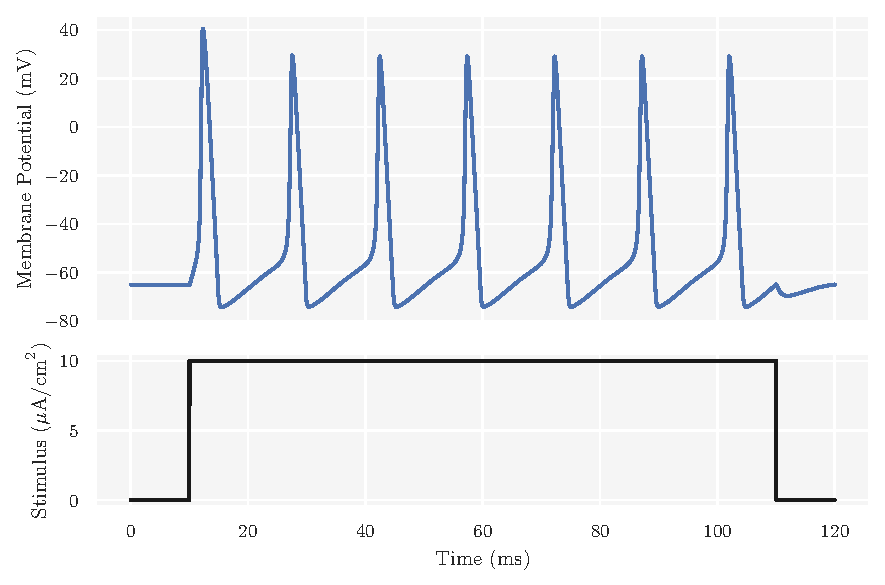
\includegraphics[scale=0.9]{hh_obs_data}
    \caption{caption}
    \label{fig:fig1}
\end{figure} 

Found locations in voltage trace for extraction of summary statistics 

\begin{figure}[H]
    \centering
    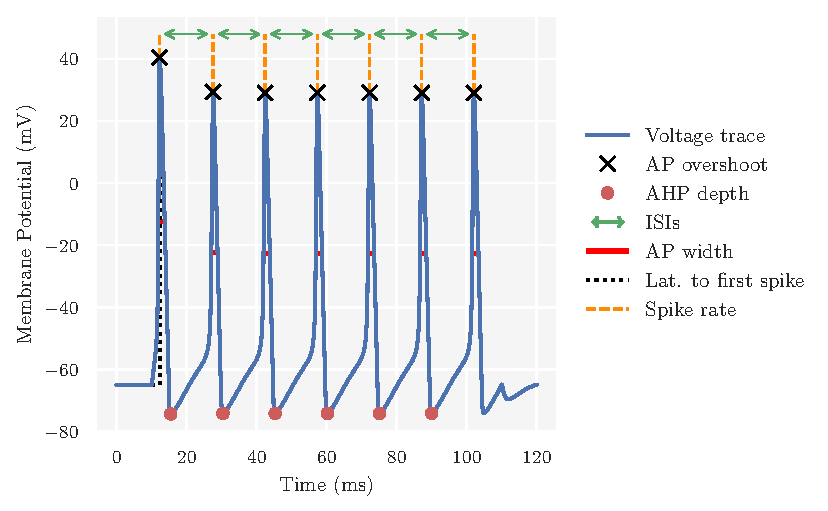
\includegraphics[scale=1]{hh_stat_extraction}
    \caption{caption}
    \label{fig:fig1}
\end{figure} 

table of observed summary statistics 

% Alternating row colors
\begin{table}[H]
  \caption{Generic table with alternating rows and different sized rulers. The number of spikes is not used as a summary statistic in and of itself, but is included to show that the statistic extraction indeed finds all spikes.}
  %\footnotesize%
  \begin{center}
    \rowcolors{2}{gray!15}{white}
    \begin{tabular}{cccc}
      \toprule
      \textbf{Summary statistic} & \textbf{Observed value} \\
      \midrule
      Number of spikes &  7 \\
      Spike rate &  0.0700 mHz \\
      Average AP overshoot & 30.7316 mV  \\
      Average AP width &  2.0501 mV \\
      Average AHP depth & -74.2234 mV \\
      Latency to first spike & 2.3000 ms \\
      Accommodation index &  $2 \cdot 10^{-17}$ \\
      \bottomrule
    \end{tabular}
  \end{center}
  \label{tab:hh_obs_sumstats}
\end{table}


\subsection{A deeper look into the statistics}

Priors for HH

\begin{figure}[H]
    \centering
    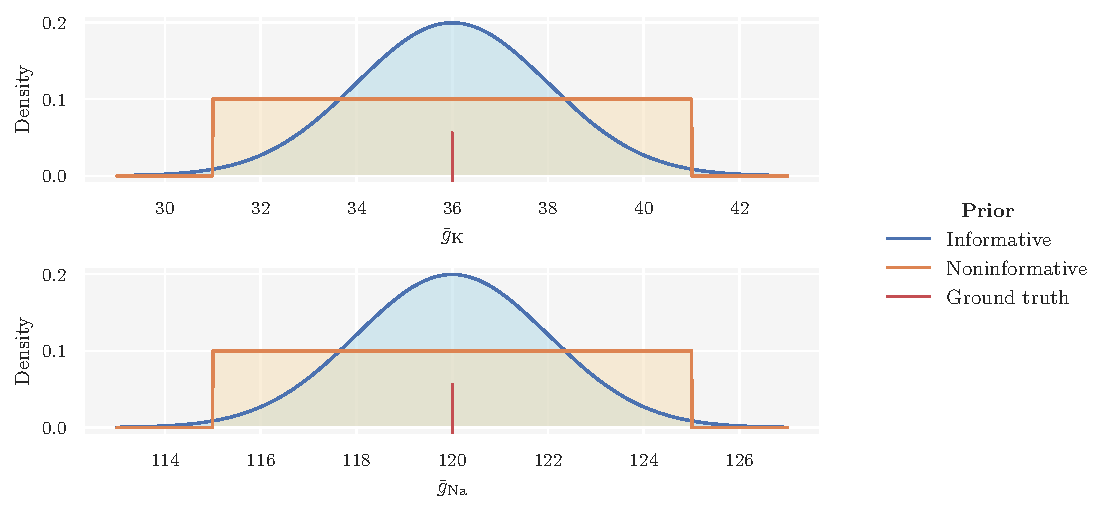
\includegraphics[scale=0.8]{hh_priors}
    \caption{caption}
    \label{fig:fig1}
\end{figure} 


Summary statistics under the (informative) prior predictive distribution (draw 2000 samples, dropna -> left with 1881 samples, but here we only plot a subset of 470 samples)

\begin{figure}[H]
    \centering
    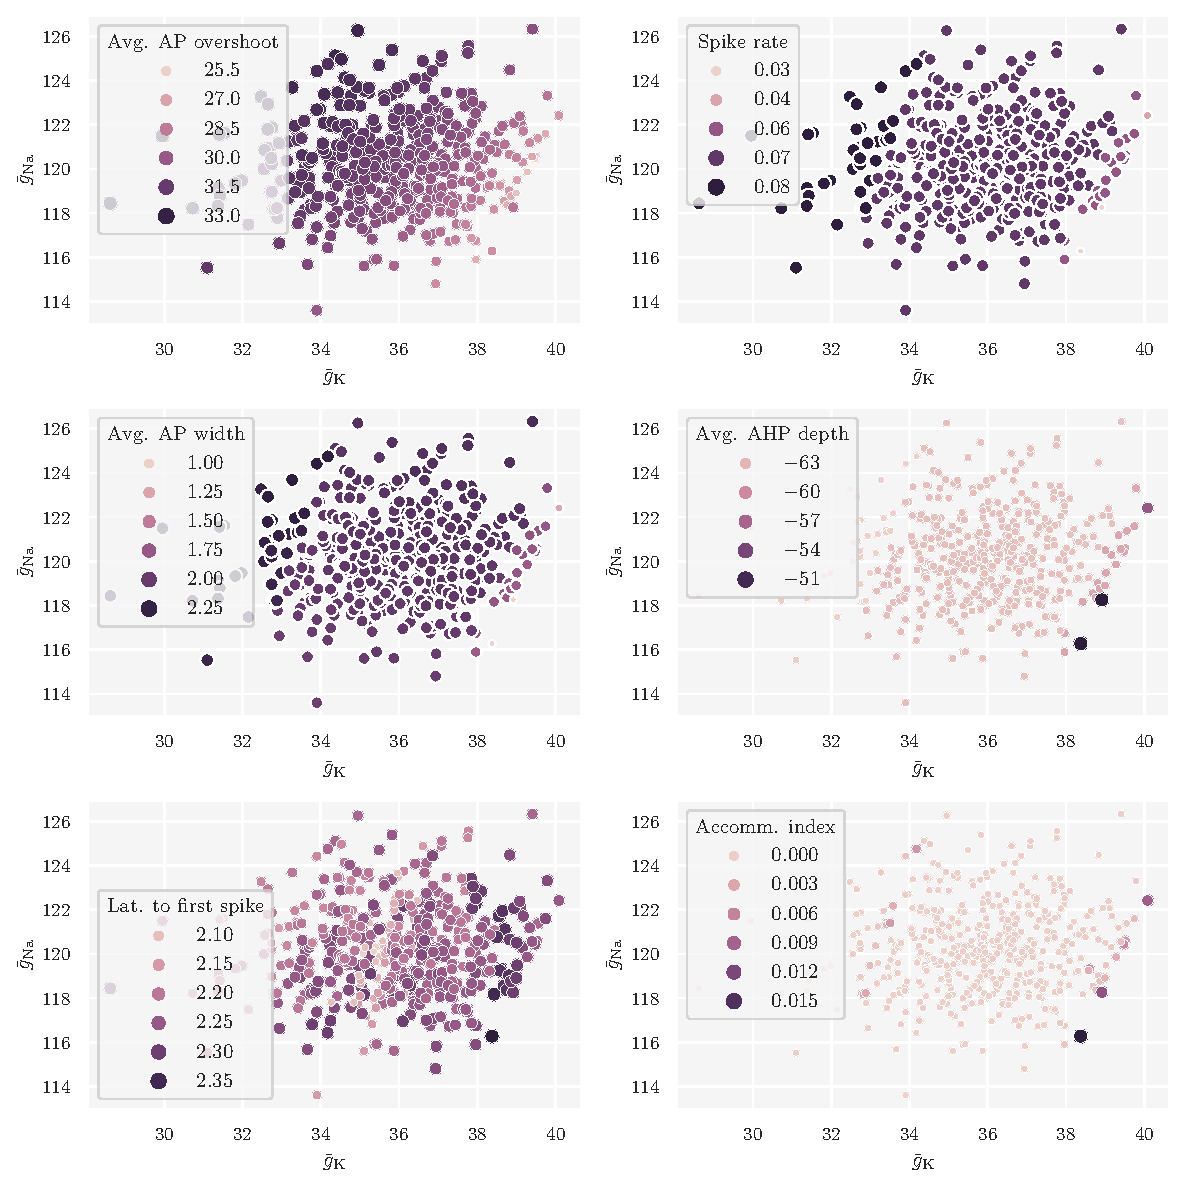
\includegraphics[scale=0.8]{hh_priorpred_sstats_normal}
    \caption{caption}
    \label{fig:fig1}
\end{figure} 


Correlation (pearson) 

\begin{figure}[H]
    \centering
    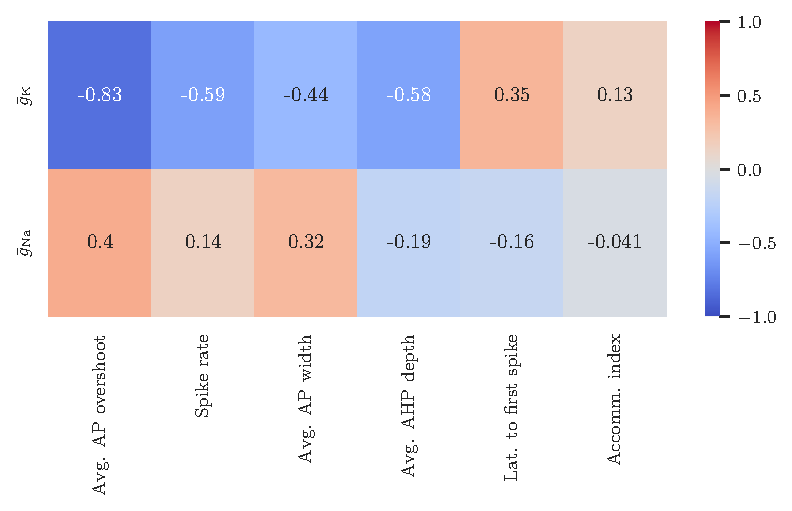
\includegraphics[scale=0.8]{hh_priorpred_corr_normal}
    \caption{caption}
    \label{fig:fig1}
\end{figure} 

weights from corr coef

\begin{figure}[H]
    \centering
    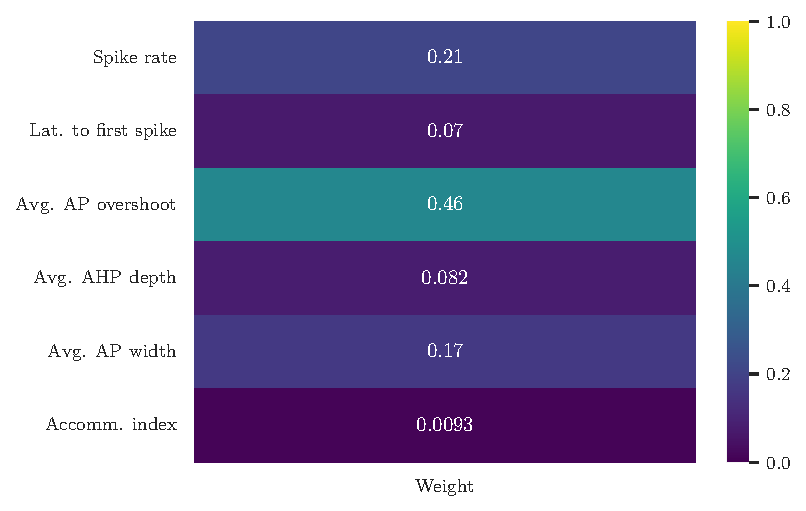
\includegraphics[scale=0.8]{hh_priorpred_weights_normal}
    \caption{caption}
    \label{fig:fig1}
\end{figure} 

Perhaps unsurprisingly, since the prior distribution does not alter the inherent relationship between the quantities, we obtain the same weights from the summary statistics generated under the noninformative prior predictive distribution. The same results as above for the noninformative prior can be found in ... ref appendix A section ...

%


\subsection{Noisy HH Data}

\begin{figure}[H]
    \centering
    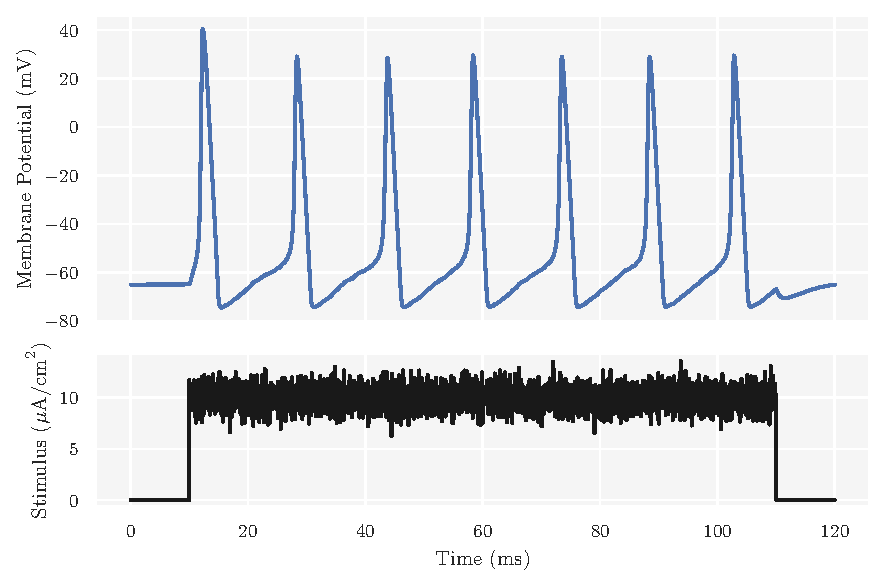
\includegraphics[scale=0.9]{hh_noisy_data}
    \caption{caption}
    \label{fig:fig1}
\end{figure} 


% Alternating row colors
\begin{table}[H]
  \caption{Generic table with alternating rows and different sized rulers. The number of spikes is not used as a summary statistic in and of itself, but is included to show that the statistic extraction indeed finds all spikes.}
  %\footnotesize%
  \begin{center}
    \rowcolors{2}{gray!15}{white}
    \begin{tabular}{cccc}
      \toprule
      \textbf{Summary statistic} & \textbf{Observed value} \\
      \midrule
      Number of spikes &  7 \\
      Spike rate &  0.0700 mHz \\
      Average AP overshoot & 30.7223 mV  \\
      Average AP width & 2.0679 mV \\
      Average AHP depth & -74.3394 mV \\
      Latency to first spike & 2.2750 ms \\
      Accommodation index &  -0.0067 \\
      \bottomrule
    \end{tabular}
  \end{center}
  \label{tab:hh_noisy_sumstats}
\end{table}



----

observed data w/o noise 

feature extraction 

plot features 

compute weights (plot correlation matrix) 

plot priors (informative, noninformative)


---

create the observed data

summary statistics of observation 

summary statistics from prior predictive

weights

(observed data with noise; same as above)

%================================================================
\section{The Brunel Network Model}
%================================================================

create the observed data

summary statistics of observation 

summary statistics from prior predictive

weights


%================================================================
\chapter{Parameter Identification with REJ-ABC}
%================================================================

%================================================================
\section{Rejection ABC Posteriors on Conductance Parameters}
%================================================================

show how Hodgkin–Huxley model is more tightly constrained by increasing numbers of data features

We also inferred HH parameters for 8 in vitro recordings from the Allen Cell Types database using the same current-clamp stimulation protocol as in our model [60, 70] (Fig. 4F, Supplementary Fig. 8). In each case, simulations based on the SNPE-inferred posterior closely resembled the original data (Fig. 4F). We note that while inferred parameters differed across recordings, some parameters (the spike threshold, the density of sodium channels, the membrane reversal potential and the density of potassium channels) were consistently more strongly constrained than others (the intrinsic neural noise, the adaptation time constant, the density of slow voltage-dependent channels and the leak conductance) (Supplementary Fig. 8). Overall, these results suggest that the electrophysiological responses measured by this current-clamp protocol can be approximated by a single-compartment HH model, and that SNPE can identify the admissible parameters.

%================================================================
\subsection{ABC Settings for Identification of Hodgkin-Huxley Parameters}
%================================================================

RMSE averaged over 10 posteriors for each quantile value. 1000 posterior samples in each posterior. 

\begin{figure}[H]
    \centering
    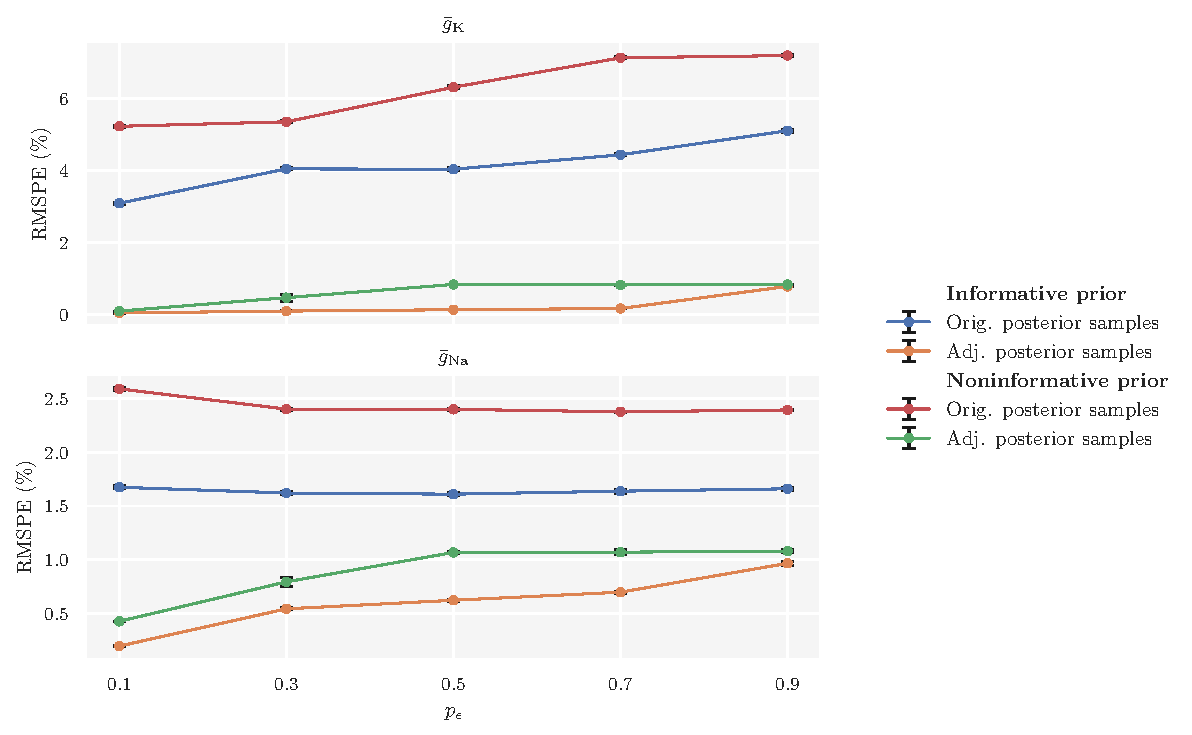
\includegraphics[scale=0.8]{RMSPE_vs_quantile}
    \caption{caption}
    \label{fig:fig1}
\end{figure} 

Run time

\begin{figure}[H]
    \centering
    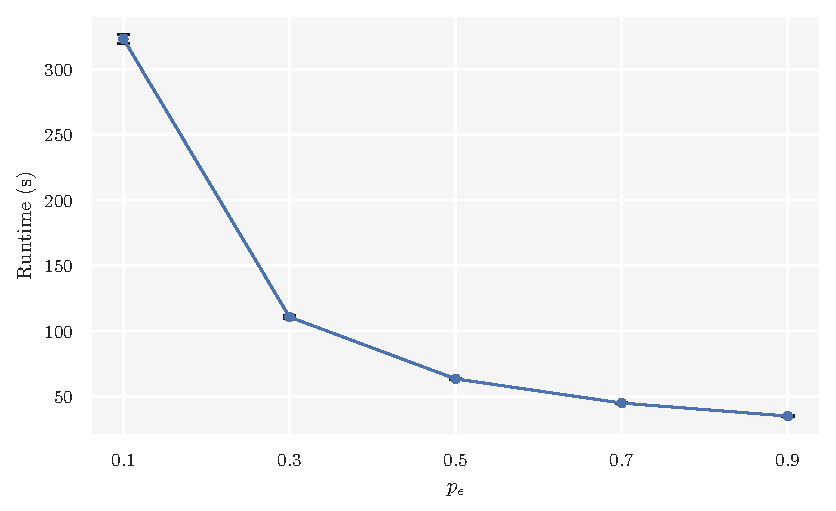
\includegraphics[scale=0.8]{comp_time_quantile}
    \caption{caption}
    \label{fig:fig1}
\end{figure}


Number of summary statistics

\begin{figure}[H]
    \centering
    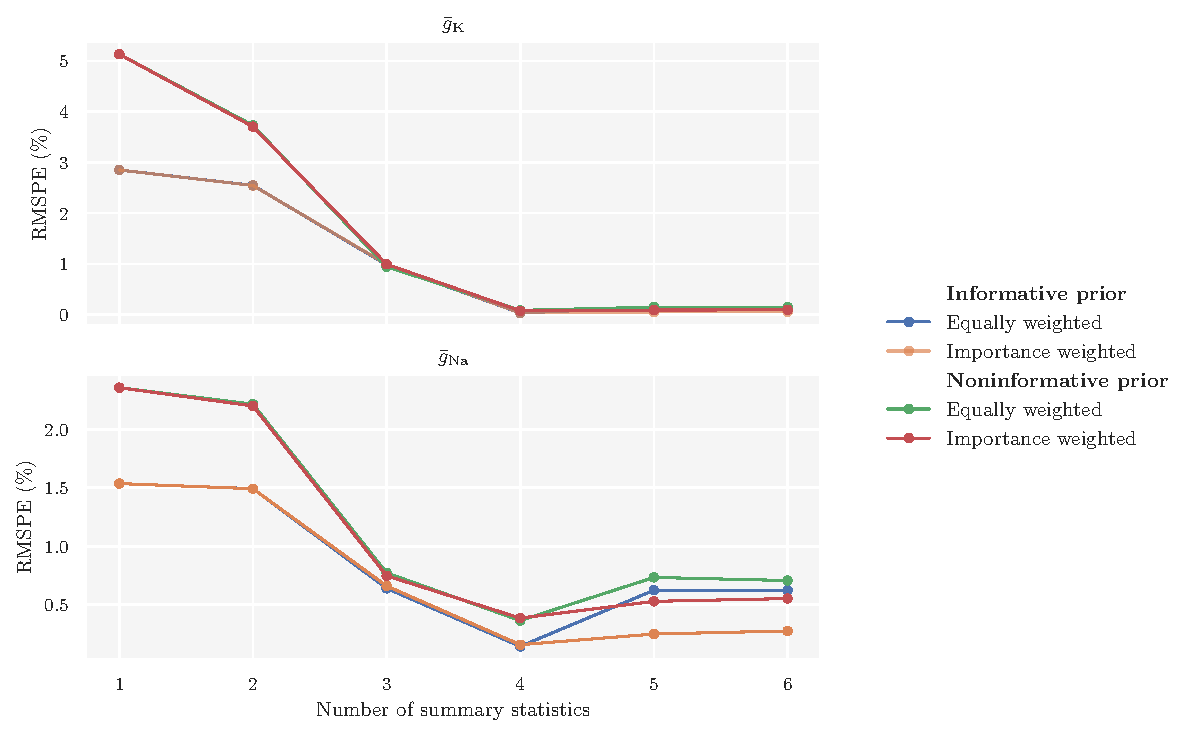
\includegraphics[scale=0.8]{RMSPE_vs_n_sumstats}
    \caption{caption}
    \label{fig:fig1}
\end{figure} 


\subsection{Summarizing Posteriors, informative priors}

Posteriors with original samples, informative prior

\begin{figure}[H]
    \centering
    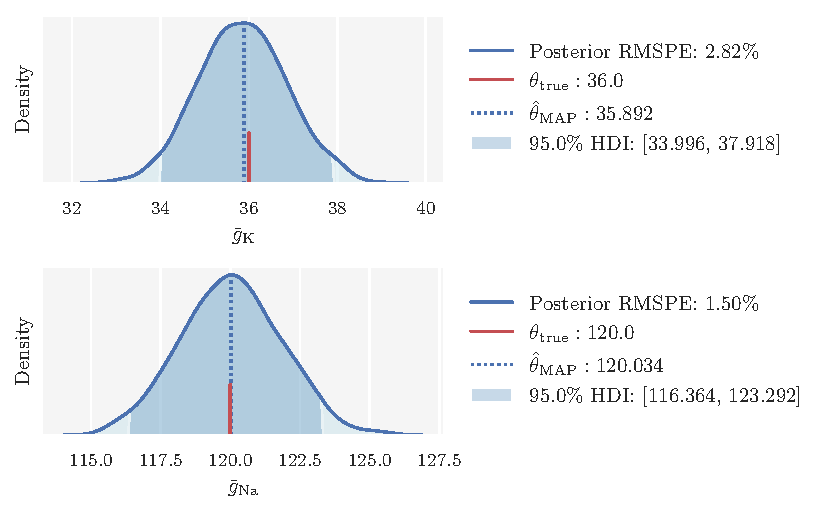
\includegraphics[scale=1]{hh_posterior_org_normal}
    \caption{caption}
    \label{fig:fig1}
\end{figure}

Correlation

\begin{figure}[H]
    \centering
    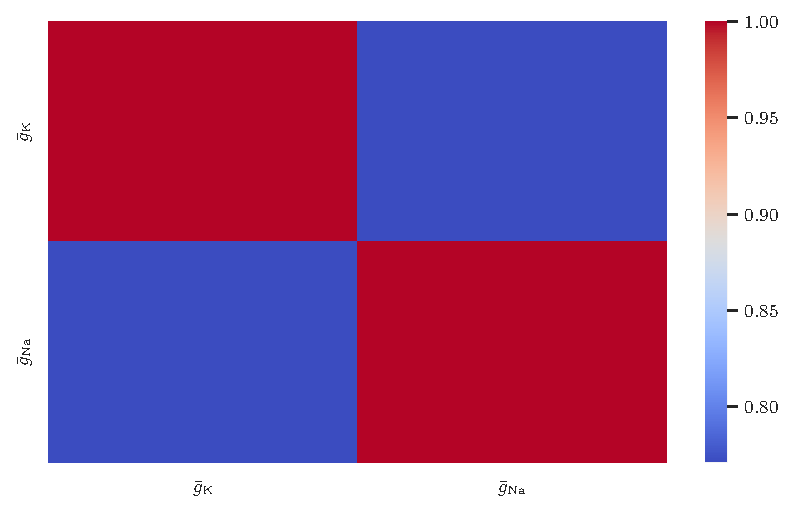
\includegraphics[scale=0.8]{hh_corr_org_normal}
    \caption{caption}
    \label{fig:fig1}
\end{figure}

Joint posterior 

\begin{figure}[H]
    \centering
    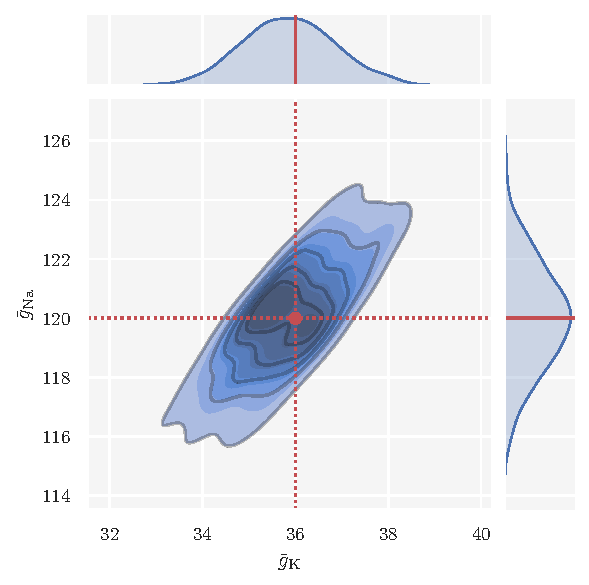
\includegraphics[scale=1.0]{hh_joint_posterior_org_normal}
    \caption{caption}
    \label{fig:fig1}
\end{figure}

Posteriors, reg adjusted samples, informative prior

\begin{figure}[H]
    \centering
    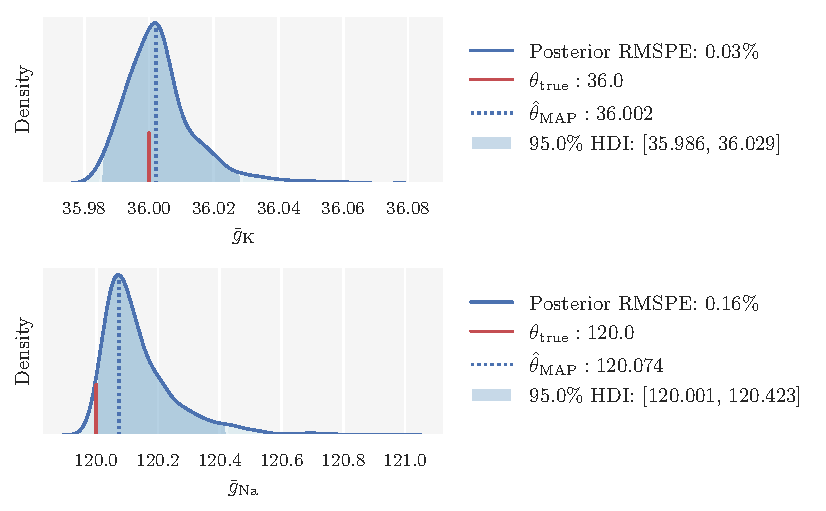
\includegraphics[scale=1.0]{hh_posterior_reg_normal}
    \caption{caption}
    \label{fig:fig1}
\end{figure}

PPC reg adjusted posterior predictive 

\begin{figure}[H]
    \centering
    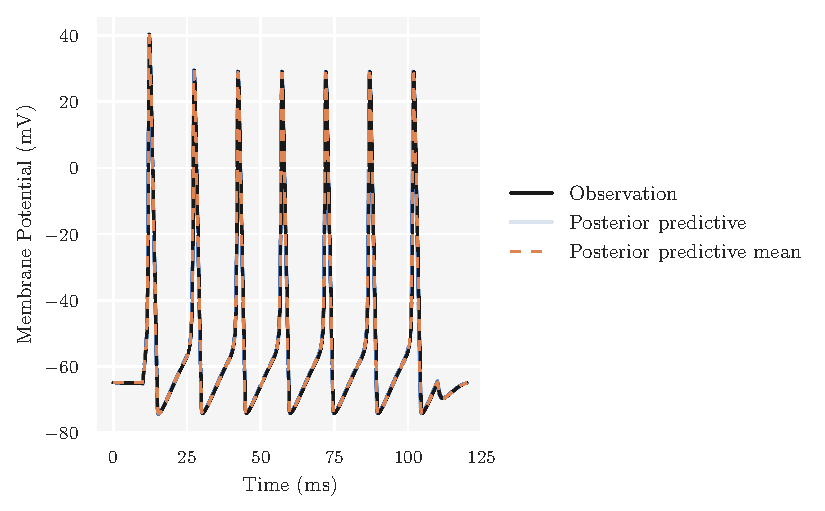
\includegraphics[scale=1.0]{hh_postpred_reg_normal}
    \caption{caption}
    \label{fig:fig1}
\end{figure}


\subsection{Summarizing Posteriors, noninformative priors}

posterior, original, noninfo prior

\begin{figure}[H]
    \centering
    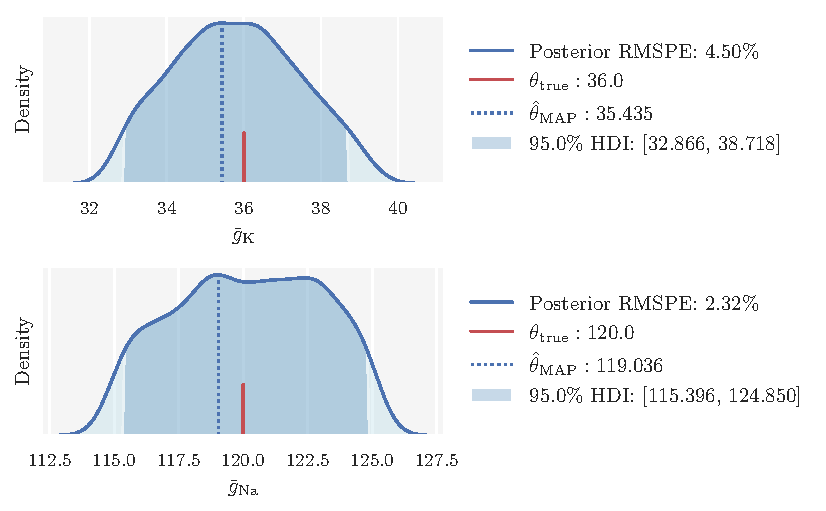
\includegraphics[scale=1.0]{hh_posterior_org_uniform}
    \caption{caption}
    \label{fig:fig1}
\end{figure}

Adjusted posterior, noninformative prior

\begin{figure}[H]
    \centering
    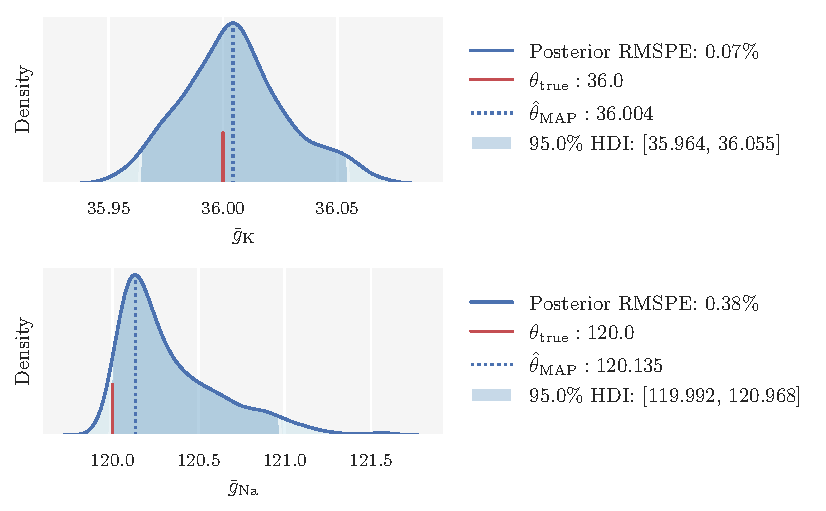
\includegraphics[scale=1.0]{hh_posterior_reg_uniform}
    \caption{caption}
    \label{fig:fig1}
\end{figure} 

PPC adjusted posterior 

\begin{figure}[H]
    \centering
    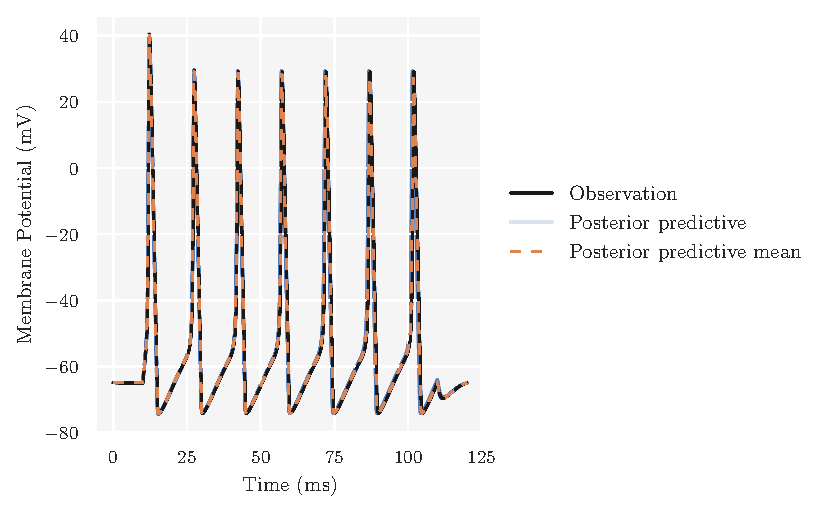
\includegraphics[scale=1.0]{hh_postpred_reg_uniform}
    \caption{caption}
    \label{fig:fig1}
\end{figure}

\subsection{Noisy observation} 

original posterior on noisy observed data

\begin{figure}[H]
    \centering
    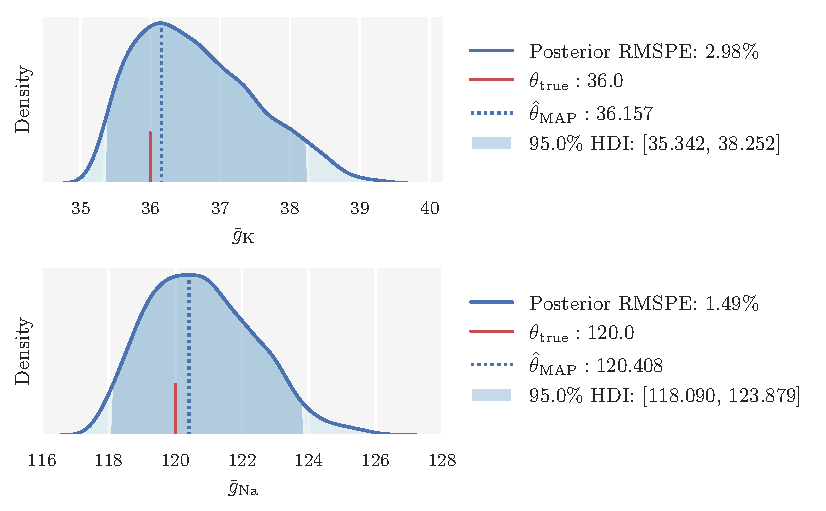
\includegraphics[scale=1.0]{hh_posterior_org_noisy}
    \caption{caption}
    \label{fig:fig1}
\end{figure} 

adjusted posterior on noisy observed data

\begin{figure}[H]
    \centering
    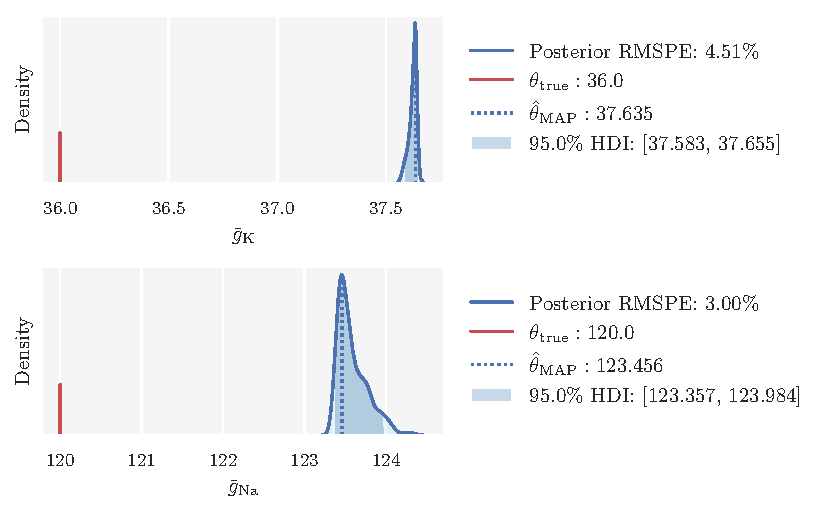
\includegraphics[scale=1.0]{hh_posterior_reg_noisy}
    \caption{caption}
    \label{fig:fig1}
\end{figure} 

ppc with reg adjusted posterior samples (100 posterior samples)


\begin{figure}[H]
    \centering
    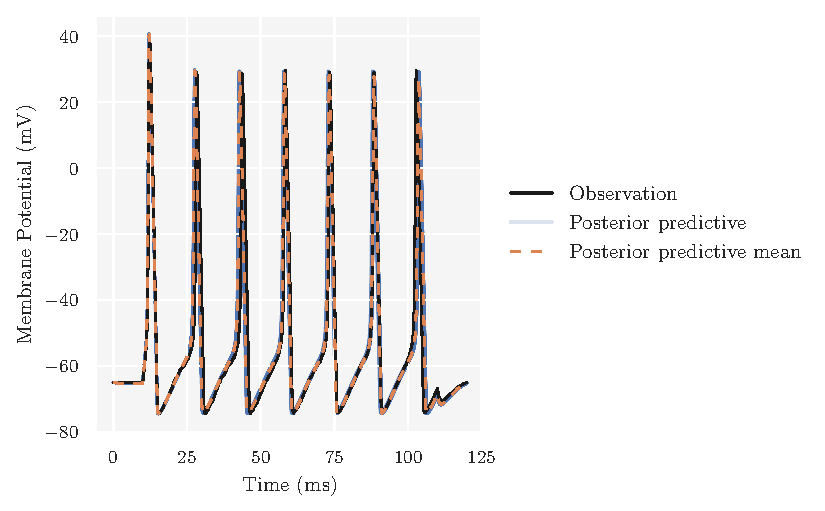
\includegraphics[scale=1.0]{hh_postpred_reg_noisy}
    \caption{caption}
    \label{fig:fig1}
\end{figure}

%================================================================
\section{ABC Settings for Identification of Brunel Network Parameters}
%================================================================

%================================================================
\section{Rejection ABC Posteriors on Synaptic Weight Parameters}
%================================================================

%================================================================
\chapter{Markov Chain Monte Carlo ABC on the Models}
%================================================================

Brunel 

\section{Observation}

observed spiketrain 

\begin{figure}[H]
    \centering
    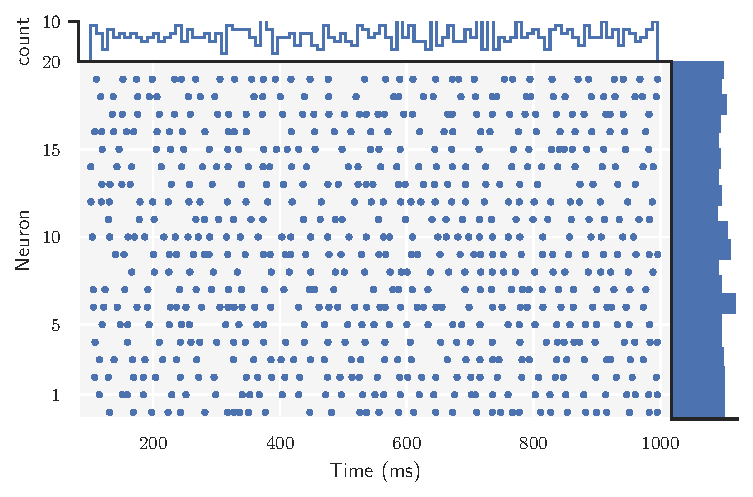
\includegraphics[scale=1.0]{brunel_obs_ai}
    \caption{caption}
    \label{fig:fig1}
\end{figure}

sum stats

%mean_firing_rate: 0.03661111111111111
%mean_cv: 0.42506007658105566
%fanofactor: 0.23413793103448277

correlation (pearson) coefficient matrix

\begin{figure}[H]
    \centering
    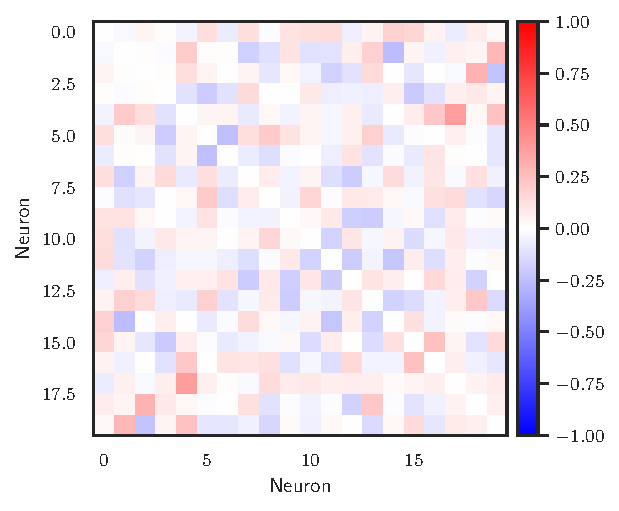
\includegraphics[scale=1.0]{brunel_obs_corr}
    \caption{caption}
    \label{fig:fig1}
\end{figure}

\section{prior pred}

priors

\begin{figure}[H]
    \centering
    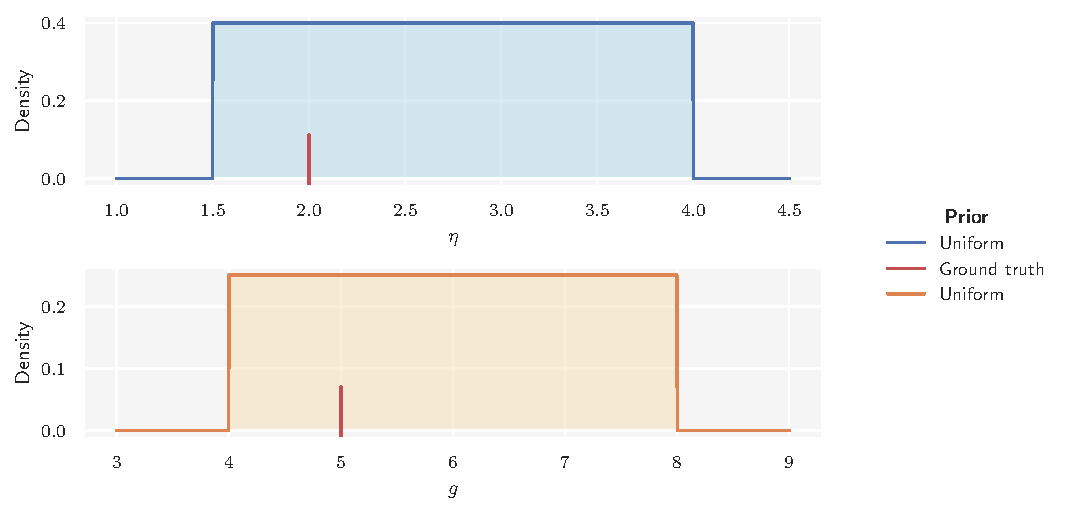
\includegraphics[scale=1.0]{brunel_priors}
    \caption{caption}
    \label{fig:fig1}
\end{figure}

sum stats scatter (500 samples)

\begin{figure}[H]
    \centering
    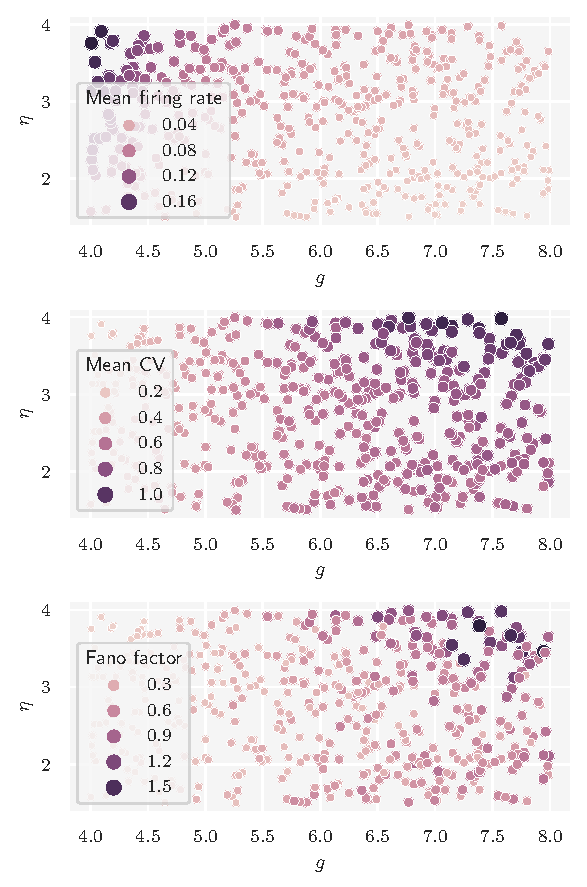
\includegraphics[scale=1.0]{brunel_sum_stats}
    \caption{caption}
    \label{fig:fig1}
\end{figure}

sum stats correlation

\begin{figure}[H]
    \centering
    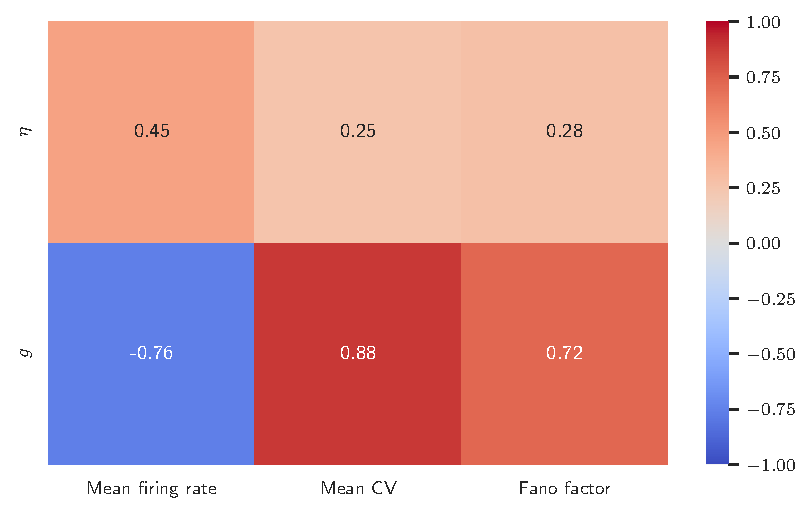
\includegraphics[scale=1.0]{brunel_sum_stats_corr}
    \caption{caption}
    \label{fig:fig1}
\end{figure}

sum stats weights

\begin{figure}[H]
    \centering
    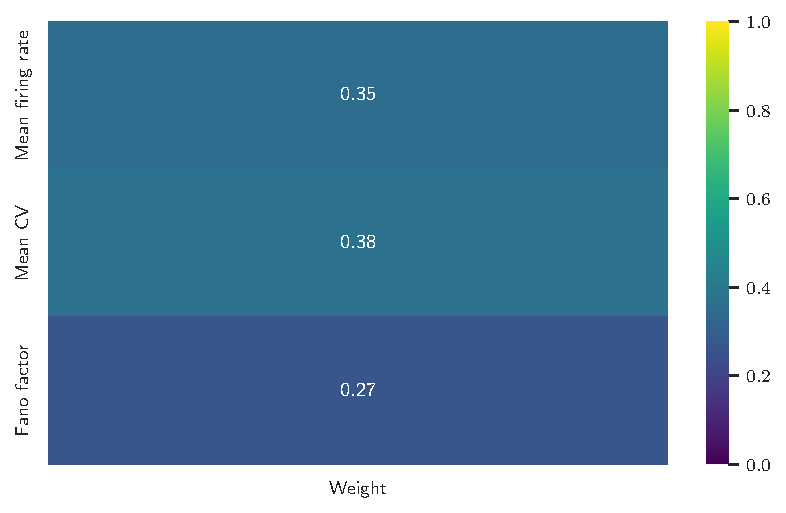
\includegraphics[scale=1.0]{brunel_sum_stats_weights}
    \caption{caption}
    \label{fig:fig1}
\end{figure}

\section{Posteriors} 

original posterior

\begin{figure}[H]
    \centering
    \includegraphics[scale=1.0]{brunel_posterior_org}
    \caption{caption}
    \label{fig:fig1}
\end{figure}


joint posterior (original)

\begin{figure}[H]
    \centering
    \includegraphics[scale=1.0]{brunel_joint_posterior_org}
    \caption{caption}
    \label{fig:fig1}
\end{figure} 

reg adjusted posterior

\begin{figure}[H]
    \centering
    \includegraphics[scale=1.0]{brunel_posterior_reg}
    \caption{caption}
    \label{fig:fig1}
\end{figure}


joint posterior (reg adjusted)

\begin{figure}[H]
    \centering
    \includegraphics[scale=1.0]{brunel_joint_posterior_reg}
    \caption{caption}
    \label{fig:fig1}
\end{figure}


%==========================================================
%------------ part 4: conclusion & future -----------------
%==========================================================

%\part{Conclusion \& Future Research}
\part{Summary \& Conclusions}
%-------------------- placeholder --------------------
%================================================================
\chapter{Summary}\label{chap:summary}
%================================================================

Mechanistic models of neural dynamics are poorly suited for inference and lead to challenging inverse problems. The objective of this thesis is to investigate the ability and utility of simulation-based inference for identifying parameters in mechanistic models of neural dynamics. We have used two simulation-based inference algorithms; (i) \textit{Approximate Bayesian Computation} (ABC) with quantile-based rejection sampling and post-sampling regression adjustment; (ii) the neural density estimator \textit{Sequential Neural Posterior Estimation} (SNPE); to infer model parameters in the Hodgkin-Huxley model \cite{HH1952} and the Brunel network model \cite{Brunel2000}. The primary focus of the study was on ABC, and SNPE results are mostly for comparison. In this chapter, we summarize our findings. 

%================================================================
\section{Correlation Analysis}
%================================================================ 

What we did, and what we found, why pearson might not be the best approach

As with covariance itself, the measure can only reflect a linear correlation of variables, and ignores many other types of relationship or correlation. 

---

correlation analysis results are indicating related results to the sensitivity analysis. Correlation analysis can be used in linear cases for the determination of important inputs on certain outputs. Here stands the condition that a meaningful number of observations are taken into account for the calculation of the empirical covariance and variances.

---

Sensitivity analysis

In a model with uncertain variables, you might want to know how much each uncertain input contributes to the uncertainty in the output. Typically, a few uncertain inputs are responsible for the lion’s share of the uncertainty in the output, while the rest have little impact. You can then concentrate on getting better estimates or building a more detailed model for the one or two most important inputs without spending considerable time investigating issues that turn out not to matter very much.

---

---

pearson correlation coefficient

Use Pearson's Coefficient of Correlation to weight importance of summary statistics.

* This is a simple approach for producing weighted statistics 
    * Method developed by H. Jung and P. Marjoram (2011) is more advanced and likely better
* The correlation coefficient, $r$, relates $Y$ to $X$ 
* The squared correlation coefficient, $r^2$, indicates the proportion of variance in $Y$ that is shared with (or accounted for) by $X$.

**Cons of using Pearson's Coefficient of Correlation:**

* Assumes:
    1. Normality of data (meaning that the data should approximate the normal distribution; most data points should tend to hover close to the mean)
    2. Homoscedasticity (means ‘equal variances’), i.e. a situation in which the variance of the dependent variable is the same for all the data.
    3. Linearity; simply means that the data follows a linear relationship. 
* (2. and 3. can be checked visually by scatter plot)
* Is sensitive to outliers; outliers can can significantly skew the correlation coefficient and make it inaccurate. Outliers are also easy to spot visually from the scatter plot

* vekte utifra sensitivitet

%================================================================
\section{Approximate Bayesian Computation}
%================================================================ 

One of the principal topics of research in likelihood-free inference is how to obtain state-of-the-art results with fewer simulations. By dissecting and studying the methods in great detail, another aim is to contribute to this research within the time and scope a master thesis permits. 

ABC: Sampling and rejection methods. In this essay, two types of ABC methods were discussed: the vanilla rejection ABC, and the more sophisticated variant Markov chain Monte Carlo ABC. There are, however, more advanced refinements that can be explored further, such as partial least squares dimension reductions for summaries and post-processing regression adjustments. An excellent point of departure for material on improvements is the video lecture by Nott [11].
• ABC: General pitfalls and remedies. ABC has been successfully applied to a wide range of problems with an complex or absent associated likelihood. There are, however, several pitfalls to be aware of. The approach is simulation intensive, requires tuning of the tolerance threshold, discrepancy function and weighting function, and suffers from a curse of dimensionality of the summary statistic [5, p. 322]. Therefore, refinements to the methods that may remedy some of the pitfalls should be explored. A point of departure could be [5] and its suggested further reading. 

---

A major methodological advance in ABC is that rather than implementing the algorithm described above, parameter sets can be more heavily weighted if the resulting simulation more closely matches the summaries of real data (Beaumont et al. 2002). In this framework, one can accept parameter values that are not as close a match to the empirical data, increasing the efficiency of the ABC. This framework has been implemented in local linear regression models (Beaumont et al. 2002) as well as other nonlinear regression approaches (Blum \& Francois 2010). 

ABC methods have several disadvantages. Firstly, the methods are highly computationally intensive, often involving billions of coalescent simulations, which may limit the parameter space explored and can lead to incorrect inference. However, the simplest ABC approaches are easily parallelizable and computational power is continuing to increase, potentially ameliorating this concern. Secondly, ABC approaches may not be efficient if the prior distributions are wide or if the type of model being considered is unlikely to generate the observed data. Under these conditions, a high proportion of parameter values will be rejected, although the local regression  approach discussed above will mitigate some of this concern. A more serious drawback is that the success of ABC inference may depend on the choice of summary statistics. If the summary statistics are not capturing enough information from the data or the relevant information for the parameters of interest, then the posterior distributions will appear similar to the prior distribution, suggesting that the data are noninformative. 


The tuning necessary is also a challenge

---

ABC methods were borne out of a need to tackle problems that defy conventional statistical methodologies. It has become clear, however, that whenever suitable Bayesian alternatives that do deal with the proper likelihood are available, ABC becomes computationally too expensive. The reason for this is primarily the fact that the representation of the posterior (as a weighted sum over Dirac delta functions) is not very efficient. So when alternatives are available, they ought to be used. In parallel to their role in computationally demanding applications, ABC techniques have, more recently, also attracted attention as an inferential framework in their own right [16,51]. From this, interesting new approaches to deal with real-world problems may well emerge [52].

In conclusion, ABC-based methods are best suited to those problems for which other likelihood-based (or exact) Bayesian inference procedures do not yet exist. This appears to still include a host of challenging and interesting problems. Many stochastic and highly structured spatio-temporal problems in ecology, epidemiology, and evolutionary genetics clearly fall into this category. The recent developments discussed above mean that ABC has become a viable new way of tackling computationally demanding parameter inference problems. Given a model—as long as we can simulate it—ABC gives us a handle to evaluate approximate posterior distributions, which then can be further evaluated. Sensitivity and robustness analyses, but also predictions of future behavior or the likely effects of any interventions or perturbations, can be analyzed by simulating the model with parameters sampled from the posterior. There is enormous scope for basing the exploration of, for example, policy or conservation measures on the available data in this way. ABC has, for example, been used in experimental design [50,53] and in synthetic biology [14,54] to generate designs of molecular pathways that exhibit certain types of behavior. In such cases, we replace the observed data, D, by a representation of the desired behavior (such as the desired abundance of a species). Then the inference procedure is used to identify the scenario for which we are most likely to observe this outcome. Such predictions then reflect the best available evidence in light of the data and the model.


%================================================================
\subsection{Regression adjustment}
%================================================================

A crucial limitation of the rejection-sampling method is that only a small number of summary statistics can usually be handled. Otherwise, either acceptance rates become prohibitively low or the tolerance $\epsilon$ must be increased, which can distort the approximation., because $\ssim$ are treated equally whenever $\rho \qty(\ssim, \sobs) \leq \epsilon$ irrespective of the precise value of $\rho \qty(\ssim, \sobs)$. Here, we introduce two improvements to existing rejection sampling methods, smooth weighting and regression adjustment. The key benefit is insensitivity of the approximation to $\epsilon$. This insensitivity permits increasing the number of summary statistics, thus potentially increasing the information extracted from the data. 

With summary statistic $T_1$, the adjustment is able to correct for the bias caused by the nonzero tolerance $\epsilon$. With summary statistic $T_2$, the tolerance is too large for accurate adjustment, although the result is still closer to the target distribution than the original.

individual components of $\theta$ are treated separately, thus not accounting for possible correlations between them. Fig. X shows that the posterior samples indeed are correlated.

Also nonlinear models have been proposed, see e.g. Blum (2010)

%================================================================
\subsection{Choice of ABC Algorithm}
%================================================================

Although neither rejection nor mcmc abc are not the best methods for sampling accurately and efficiently, and scale poorly to higher dimensional problems, they provide a solid basis for understanding more sophisticated/refined sampling schemes and post-hoc adjustments. They showcase that abc provides a robust framework for parameter identification


The efficiency of the method is, however, largely dependent on the efficieny of the simulator model. As an informal side note: all results in this thesis were produced on a personal laptop. Inference on the most time-consuming model, the Brunel network, took about 2 hours with ABC (2000 simulations) and 2.5 hours with SNPE (running 1000 (adaptively proposed) simulations to train the network). 

rejection abc not efficient if the prior .. posterior. MCMC, as discussed in theory section, improves on this by ... 

There are more advanced importance sampling ABC methods that builds on the MCMC approach: SMC, PMC, HMC - ABC (link to papers)

Perhaps the most notable difference between the approach of ABC and SNPE, is that SNPE uses \textit{all} model simulations to train the network opposed to ABC that usually ends up rejecting most of the simulations. Another important difference is that once the network is trained, it can be used to predict posterior on any empirical data with just one pass through the network. Whereas ABC would need to be performed again when presented with another set of empirical data. 

%================================================================
\subsection{Choice of Summary Statistics}
%================================================================

The choice of summary statistics is vital in determining the outcome of the inverse modelling with ABC. The set of statistics must effectively encode all phenomena of the original data that the experimenter wishes to be modelled. 

For our purposes, requiring that S.Y/ be sufficient is problematic because we
can’t examine an unknown or intractable likelihood to determine if the Fisher- Neyman Factorization Theorem holds. Although there are a growing number of different strategies for resolving the sufficiency problem [42], the most common approach has been to select a large set of summary statistics and hope that this set of statistics is large enough that it is at least close to being jointly sufficient for the parameters of interest. While adding more summary statistics to this set will

tend to provide more information about theta, sufficiency can still never be guaranteed, and some summary statistics may provide identical information about the model parameters. When a set of summary statistics are not sufficient for the parameters, then the influence of the information conveyed by the observed data will be weaker, resulting in posterior distributions that are inaccurate, particularly with respect to the degree of variability in the estimated posteriors


---

A further motivation for this approach is that real-world experiments often are interested in capturing summary statistics of the experimental data. 

In practice, in order to maintain the acceptance probability at manageable levels, we typically transform the data into a small number of features, also known as summary statistics, in order to reduce the dimensionality D. If the summary statistics are sufficient for inferring $\theta$, then turning data into summary statistics incurs no loss of information about $\theta$ (for a formal definition of sufficiency, see e.g. Wasserman, 2010, definition 9.32). However, it can be hard to find sufficient summary statistics, and so in practice summary statistics are often chosen based on domain knowledge about the inference task. A large section of the ABC literature is devoted to constructing good summary statistics (see e.g. Blum et al., 2013; Charnock et al., 2018; Fearnhead and Prangle, 2012; Prangle et al., 2014, and references therein).


figure x shows how the Hodgkin-Huxley model is more tightly constrained by increasing the number of summary statistics. Though, if we use summary statistics that do not capture relevant information for the parameters of interest it might lead to worse inference, as seen in the figure for the latency to first spike and accommodation index statistics.  

However, this result showcases the importance of carrying out a sensitivity analysis on the model parameters. Uncertainpy

explanatory power

the success of ABC inference depends on the choice of summary statistics. If the summary statistics are not capturing enough information from the data or the relevant information for the parameters of interest, then the posterior distributions will appear similar to the prior distribution, suggesting that the data are noninformative. 

--- 
To deal with high dimensional data, ABC algorithms typically reduce them to lower dimensional summary statistics and accept when simulated summaries are close to the observed summaries. 

A crucial limitation of the ABC approach is that only a small number of summary statistics can usually be handled. Otherwise, either acceptance rates or become prohibitively low or the tolerance must be increased, which can distort the approximation. The problem is related to the general issue of the curse of dimensionality: many statistical tasks are substantially more difficult in high dimensional settings. 


%================================================================
\subsection{Choice of Distance Metric}
%================================================================ 

While the choice of summary statistics is of primary importance, the choice of distance metric can also have a substantial impact on the quality of the posterior approximation. In the present study, we used the Euclidean distance. This amounts to a circular acceptance region, as illustrated by \autoref{fig:abc_illustration}, which implies independence and identical scales of the summary statistics. Technically, because of the dimensionality of the summary statistics vectors we used, the acceptance regions were spherical. However, we stick with the circular analogy as it is easier to conceptualize. In order to suppress domination of the summary statistics with largest scale, we used a weighted version of the Euclidean distance that scaled the summary statistics with their respective standard deviation estimated from the prior predictive distribution. Moreover, we also weighted the importance of the summary statistics based on the correlation analysis. Despite these efforts, the Euclidean distance might not have the acceptance region that results in the most accurate ABC posterior approximation. If we, reasonably, suppose that the different summary statistics are dependent and on different scales, their true distribution under the model may be better represented by an elliptical acceptance region rather than a circular. The Mahalanobis distance is an example of a distance metric with elliptical acceptance region. However, the different levels of information encoded by the different summary statistics make finding the optimal acceptance region a challenge. Even with different scales and dependences, a circular acceptance region might result in a more accurate ABC posterior approximation than an elliptical region if the circular is better tied up with the most informative statistics. How the best acceptance region is connected with the choice of summary statistics is discussed in detail by Prangle in \cite{prangle_distance}. 



%================================================================
\section{Identifiability}
%================================================================  

To assess the goodness of the inferred solution, we have generated an image with known con- figuration and compared the estimated posterior with the input configuration. We find that ABC produced a reliable approximate posterior that was consistent with the input param- eter values and mapped the correlation between simulation parameters. The ABC method with its PMC implementation is thus promising for numerous forward modeling problems in cosmology and astrophysics.

To assess the goodness of the inferred posterior, we have discussed several considerations for good performance, including the MAP estimate, highest density interval and posterior predictive checks. Particularly, since the ground truth parameters are known, we have used an error measure that considers the width of the posterior by averaging over the posterior, RMSPE.

see HH ABC 

We will assess the identifiability of the potassium and sodium conductance parameters by examining the width of the resulting posterior estimates. A wide, flat posterior on a parameter indicates a large number of equally optimal values, which suggests that the parameter may be unidentifiable.

Application of these new techniques also allows us to explore the issue of model identifiability. By examining posterior distributions over model parameters, we can quantify and characterize model uncertainty, which can either inform us as to the ability of our data to constrain the model or the degree of biological variability in the system, as we outline below.

If a cellular model were to have a non-unique optimal parametrization, with either several or infinitely many equally likely possibilities, the model may be deemed 'unidentifiable'. Unidentifiability can be divided into two types: structural unidentifiability, where the model is overly complex to describe the system (this is often called over-parametrization), and practical unidentifiability, where there are not enough data to fully constrain the model. Distinguishing between the two types of unidentifiability can be important for experimental design. Pinpointing a structural  unidentifiability, which is characterized by a functional relationship between several parameters (and thus infinitely many equally optimal parametrizations), may be cause for concern, and prompt changes in model formulation before attempting further experimentation. However, if there is a high degree of prior faith in the model formulation, this may instead suggest a biologically important redundancy in the system characterized by the functional relationship between biophysical parameters. Practical unidentifiability, on the other hand, may inform how additional experimental data might be collected in an effort to further constrain the model, or may be a representation of inherent variability of the biophysical parameters in the experimental system. 

%================================================================
\subsection{The Hodgkin-Huxley Model}
%================================================================ 

Hodgkin-Huxley, reason for why $\bar{g}_\mathrm{K}$ is better constrained than $\bar{g}_\mathrm{Na}$:

The sensitivity analysis reveals that the variance in the membrane potential mainly is due to the uncertainty in two parameters: the maximum conductance of the $\mathrm{K}^+$ channel, $\bar{g}_\mathrm{K}$, and the $\mathrm{Na}^+$ reversal potential, $E_\mathrm{Na}$.

A similar study of using ABC to constrain the Hodgkin-Huxley model parameters was carried out in .. hh abc .. They primarily focused on constraining the rate parameters, and were also able to successfully identify the parameters.  

Indicating that Abc is a viable method for parameter identification in the many models using the hodgkin-huxley formalism

%================================================================
\subsection{The Brunel Network Model}
%================================================================ 

Brunel 

Able to accurately predict summary statistics ...

Indicates that $\eta$ is not dominant in determining the dynamics of the SR state. 

Supported by the findings of (uncertainpy paper), where a sensitivity analysis of the Brunel model parameters was carried out. In the SR state, (uncertainpy paper) found that the Brunel network is most sensitive to the synaptic delay $D$ (which is kept constant in our results). However, the network was also found to be more sensitive to $g$ than $\eta$ in the SR state. 

In the AI state, the network was found to be most sensitive to the relative strength of inhibitory synapses $g$. The $\eta$ parameter also plays a role in the AI state, but not as much as $g$. The synaptic delay $D$ plays no role. 

SNPE both Brunel states

Expected unidentifiability: SR state Brunel, biophysical explanation. In this state of neurons firing almost synchronously at high rates, the spiking activity is to a large extent generated by the network population itself due to the recurrent connections. (Positive feedback). Thus, will the external input play a lesser role. The $\eta$ parameter that describes the amount/strength of external input (background rate) will therefore be overshadowed by the internal drive of the activity if the internal rate is significantly larger. Also seen in/confirmed by Uncertainpy analysis.

%================================================================
\subsection{Constraining Model Parameters}
%================================================================ 


When fitting mechanistic models to data, it is common to target summary features to isolate specific behaviors, rather than the full data. For example, the spike shape is known to constrain sodium and potassium conductances (Druckmann et al., 2007; Pospischil et al., 2008; Hay et al., 2011). When modeling population dynamics, it is often desirable to achieve realistic firing rates, rate-correlations and response nonlinearities (Rubin et al., 2015; Bittner et al., 2019), or specified oscillations (Prinz et al., 2004). Choice of summary features might also be guided by known limitations of either the model or the measurement approach, or necessitated by the fact that published data are only available in summarized form.  In all cases, care is needed when interpreting models fit to summary features, as choice of features can influence the results (Blum et al., 2013; Jiang et al., 2017; Izbicki et al., 2019).


While there is no universally accepted automated means to assess identifiability, many different methods, such as parameter sensitivity analysis and analysis of curvature of an objective function, have been applied to cardiac cell models.   


- parameter sensitivity analysis: uncertainpy 

- analysis of curvature of an objective function: druckmann

... have been applied to models of neural dynamics

\textbf{Relevant papers:}

H. Jung and P. Marjoram (2011). "Choice of Summary Statistic Weights in Approximate Bayesian Computation". \url{https://www.ncbi.nlm.nih.gov/pmc/articles/PMC3192002/}

* Develops a Genetic Algorithm that computes how one should weight the summary statistics 

* Fairly advanced, so we won't implement their approach, but should be mentioned in thesis

%================================================================
\section{Scalability}
%================================================================ 

We now turn to a discussion of scalability ... not investigated in this thesis. 

SNPE has also been applied by the creators on several models of neural dynamics in \cite{SNPE_applied}. They were able to use SNPE to identify up to ... parameters. (scalability)


We have only demonstrated the success of simulation-based inference on low dimensional problems, i.e., few parameters to identify. 

state-of-the-art V1 allen model, 1500 free parameters. Although it might be excessive to infer all of these parameters at once, the problem will nonetheless be high-dimensional. 

ABC have been shown to scale poorly to higher dimensions

SNPE have been demonstrated to obtain good results for systems with about X free parameters (ref paper), but has yet to demonstrate scalability to problems like the V1 model. In its current state, one of the principal investigators behind SNPE, J. Macke, stated that SNPE is only able to infer up to a couple of dozen parameters, depending on the problem (ref: in conference).


\section{Notes}

In this thesis, we have formulated a framework for the inverse modelling of neural dynamics based upon an algorithm using rejection ABC with post-hoc corrections through regression adjustment. We characterized the properties of this method when applied to models typically used in computational neuroscience; a biophysically detailed neuron model (HH model) and a neural network of point neurons model (Brunel model). Examination of the outcomes of the rejection ABC algorithm indicated that parameter estimates converge to yield best fit approximations to the summary statistics of empirical data and provide constraints upon the parameter estimates associated with a data dependent reduction in the estimated posterior precision. 

To assess the validity of the procedure we tested for predictive validity. These results demonstrated that the model inversion and comparison approach are able to reliably identify the model that generated the data. 

%================================================================
\chapter{Conclusions}\label{chap:conclusions}
%================================================================

We investigated how simulation-based inference can be applied to inverse modelling of mechanistic models of neural dynamics, where the likelihood is unavailable or intractable. In particular, we explored the ability of approximate Bayesian computation (ABC) and neural density estimation (NDE) to identify the conductance parameters in the Hodgkin-Huxley model and the synaptic weight parameters in the Brunel network model. 

We discussed an implementation of the rejection ABC algorithm with quantile-based tolerance and post-sampling local linear regression adjustment. Even though rejection ABC just sample proposal parameters from the prior densities, we were, in general, successful in identifying the model parameters of interest. By applying local linear regression adjustment, we obtained narrow posterior densities with the ground truth values of the parameters in regions of high posterior density. The posterior error decreases in the limit of small tolerances. With regression adjustment, we found that we could accept more simulations without sacrificing substantial accuracy for the model parameters that were the most constrained by the summary statistics. The choice of summary statistics is crucial for the performance of ABC. In practice, the success of ABC relies on expert-crafted low-dimensional summary statistics that constrain the model parameters of interest. Although the rejection ABC approach were able to perform efficiently, in particular on the Hodgkin-Huxley model, and recover the ground truth parameters, more advanced sampling algorithms with better proposal mechanisms should be considered. The accurate results we were able to obtain with the simple rejection sampler implies that even better results can be expected by using more advanced samplers. 

We compared the rejection ABC algorithm with the NDE machine learning tool Sequential Neural Posterior Estimation (SNPE), which trains an artificial neural network to map features of observed data to posteriors over parameters by using adaptively proposed model simulations. Inference on the Brunel network model demonstrates the power and flexibility of SNPE; by training on simulations that included the parameter ranges for two of the network states, SNPE was able to accurately predict posteriors that corresponded to the network's state in the observed data. The advantage of the SNPE approach is that once trained, the network can be applied to any observed data and estimate the posterior densities over model parameters with only a single pass through the network. 


%Recently, there have been developed simulation-based inference machine learning algorithms using \textit{artificial neural network-based conditional density estimators}. In particular, the  \textit{Sequential Neural Posterior Estimation} (SNPE) algorithm targets parametrically learning the posteriors over model parameters by using adaptively proposed model simulations instead of likelihood calculations. More specifically, the algorithm trains a Bayesian mixture-density network (MDN) to learn the association between data, or summary statistics of the data, and underlying parameters. Instead of filtering out simulations, as ABC algorithms do, SNPE uses \textit{all} simulations to train the MDN to identify admissible parameters. Once trained, the network can then be applied to observed data to derive the posterior densities over the parameters of the simulator model. 


A limiting factor of the simulation-based approach to inference is that the algorithms are simulation intensive. Consequently, the efficiency of an algorithm predominantly depends on the computational demands of the simulator. There are also challenges (and opportunities) ahead in scaling and automating simulation-based inference approaches. However, the frontier of simulation-based inference as a methodological research field is rapidly advancing. This activity is promising for the numerous inverse modelling problems in neuroscience. The generality of the simulation-based inference methods allows them to be applied to a wide range of computational investigations in need of improved inference quality. In addition to being able to aid in designing better models of neural dynamics, simulation-based inference may ultimately help to bridge the gap between mechanistic hypotheses and experimental neural data. 


%However, simulation-based inference is promising for the numerous inverse modelling problems in neuroscience. The generality of the methods allows them to be applied to a wide range of computational investigations in need of improved inference quality. In addition to being able to aid in designing better models of neural dynamics, simulation-based inference may help to bridge the gap between mechanistic hypotheses and experimental neural data. 

%A limiting factor of the ABC methods are that they are simulation intensive and the efficiency of the procedure depends on the the computational demands of the simulator. ABC has been successfully applied to a wide range of problems with an complex or absent associated likelihood. There are, however, several pitfalls to be aware of. The approach is simulation intensive, requires tuning of the tolerance threshold, discrepancy function and weighting function, and suffers from a curse of dimensionality of the summary statistic. 

% Until recently, scientists confronted with inverse problems and a complex simulator as a forward model had little recourse other than to choose ABC or methods based on classical density estimation techniques. While these approaches have served some domains of science quite well, they have relied heavily on the labor-intensive process of experts providing powerful summary statistics. As a result, there is a frontier beyond which these traditional methods are less useful and new techniques are needed.

% The term likelihood-free inference has served as a point of convergence for what were previously disparate communities, and a new lingua franca has emerged. This has catalyzed significant cross-pollination and led to a renaissance in simulation-based inference. The advent of powerful ML methods is enabling practitioners to work directly with high-dimensional data and to reduce the reliance on expert-crafted summary statistics. New programming paradigms such as probabilistic programming and differentiable programming provide new capabilities that enable entirely new approaches to simulation-based inference. Finally, taking a more systems-level view of simulation-based inference that brings together the statistical and computational considerations has taken root. Here active learning is leading the way, but we expect more advances like this as simulation-based inference matures.

%The rapidly advancing frontier means that several domains of science should expect either a significant improvement in inference quality or the transition from heuristic approaches to those grounded in statistical terms tied to the underlying mechanistic model. It is not unreasonable to expect that this transition may have a profound impact on science.



%================================================================
\chapter{Future Research}\label{chap:future}
%================================================================

%Armed with these insights .. conclusion

We here provide an outline of potential future research building off of the present work.  

In this study, we have only investigated low-dimensional problems, i.e., inferential tasks with few parameters to identify. However, 

Recent studies, see e.g. Skaar et al. 

%Concluding remarks.

Possible future studies. Reference other relevant studies. 

Use more refined ABC methods
(SMC ABC ++, SNPE and SNL)

Compare with principled modelling; thermodynamic models

Metamodelling

Scalability 

Check if is scalable in the number of parameters;
Higher dimensional problems (more parameters to estimate)

Try to make contact between real-world experimental data and mechanistic models of neural dynamics. 


%==========================================================
%--------------------- appendices -------------------------
%==========================================================

\appendix           % "Chapter" is renamed "Appendix"
\part*{Appendices}
\addcontentsline{toc}{part}{Appendices}


%\appendixpage       % Similar to \part*{Appendices}, but appears in TOC

%--------------------- appendix A --------------------
%================================================================
%\chapter{Selection of Standard Probability Distributions}\label{sec:Appendix A}
\chapter{Additional Results}\label{sec:Appendix A}
%================================================================


\begin{figure}[H]
    \centering
    \includegraphics[scale=1.0]{hh_different_gs}
    \caption{Simulation of action potentials with the Hodgkin-Huxley simulator for different values of $\gbarK$ and $\gbarNa$ (stated in the legend). The rest of the parametrization is given by \autoref{tab:hh_model_parameters}.
    }
    %\label{fig:hh_different_gs}
\end{figure}


\begin{figure}[H]
    \centering
    \includegraphics[scale=0.7]{hh_priorpred_sstats_uniform}
    \caption{Similar to \autoref{fig:hh_priorpred_sstats_normal}, only with summary statistics simulated under the joint noninformative prior distribution. Of the 2000 samples generated, 1703 were well-defined. Here a subset of 425 samples is shown.}
    %\label{fig:fig1}
\end{figure} 

% subfigure
\begin{figure}[H]
\centering
\subfloat[]{{\includegraphics[scale=0.65]{hh_priorpred_corr_uniform}}}
\qquad
\subfloat[]{{\includegraphics[scale=0.65]{hh_priorpred_weights_uniform}}}
\caption{Similar to \autoref{fig:hh_weights_normal}, but with samples from the joint noninformative prior distribution. \textbf{(a)} The pairwise Pearson's correlation coefficients. \textbf{(b)} Importance weights calculated from the correlation coefficients (summed to 1).
}
%\label{fig:hh_weights_uniform}
\end{figure}


 
%REJ-ABC hyperparam study 

%Run time

\begin{figure}[H]
    \centering
    \includegraphics[scale=0.8]{comp_time_quantile}
    \caption{Illustration of computational run time for obtaining 1000 posterior samples with the HH simulator vs. tolerance quantile, i.e., the proportion of simulations that are accepted.}
    \label{fig:runtime}
\end{figure}

%num of pilot study simulations 

\begin{figure}[H]
    \centering
    \includegraphics[scale=0.8]{pilot_eps_nsims}
    \caption{Estimated tolerance $\epsilon$ vs. the number of simulations in the pilot study. Here, both summary statistic scales and weights are set to 1 when calculating the distance, so the estimates might not be representative for all use cases.}
    %\label{fig:fig1}
\end{figure} 

%num of posterior draws

%\begin{figure}[H]
%    \centering
%    \includegraphics[scale=0.8]{RMSPE_vs_nsamples}
%    \caption{caption}
%    \label{fig:fig1}
%\end{figure} 

\begin{figure}[H]
    \centering
    \includegraphics[scale=1.0]{hh_posterior_org_uniform}
    \caption{Original rejection ABC posteriors over the Hodgkin-Huxley model parameters $\gbarK$ (top) and $\gbarNa$ (bottom) with noise-free observed voltage trace. Here, the parameter proposals were sampled from the joint noninformative prior distribution. The dark shaded region indicates the 95\% HDI and the dotted line the MAP estimate. The ground truth is indicated by the red line. The legend states the numerical values for each of these, in addition to the RMSPE in the posterior.}
    %\label{fig:fig1}
\end{figure}


\begin{figure}[H]
    \centering
    \includegraphics[scale=1.0]{hh_postpred_reg_uniform}
    \caption{Graphical posterior predictive check comparing the observed voltage trace to simulated data predicted by the Hodgkin-Huxley model under the regression adjusted joint posterior predictive distribution that is shown as marginal posteriors in \autoref{fig:hh_posterior_reg_uniform}.}
    %\label{fig:fig1}
\end{figure}


\begin{figure}[H]
    \centering
    \includegraphics[scale=1.0]{hh_posterior_org_noisy}
    \caption{Original rejection ABC posteriors over the Hodgkin-Huxley model parameters $\gbarK$ (top) and $\gbarNa$ (bottom) with noisy observed voltage trace. Here, the parameter proposals were sampled from the joint informative prior distribution. The dark shaded region indicates the 95\% HDI and the dotted line the MAP estimate. The ground truth is indicated by the red line. The legend states the numerical values for each of these, in addition to the RMSPE in the posterior.}
    \label{fig:hh_posterior_org_noisy}
\end{figure} 


\begin{figure}[H]
    \centering
    \includegraphics[scale=1.0]{brunel_posterior_org}
    \caption{Original rejection ABC posteriors over the Brunel network model parameters $\eta$ (top) and $g$ (bottom) with observed data from the AI state. The dark shaded region indicates the 95\% HDI and the dotted line the MAP estimate. The ground truth is indicated by the red line. The legend states the numerical values for each of these, in addition to the RMSPE in the posterior.
    }
    %\label{fig:fig1}
\end{figure}

%Brunel joint posterior (original) (REMOVE?)

%\begin{figure}[H]
%    \centering
%    \includegraphics[scale=1.0]{brunel_joint_posterior_org}
%    \caption{caption}
%    \label{fig:fig1}
%\end{figure} 




%--------------------- appendix B --------------------
%================================================================
\chapter{Abbreviations and Units}\label{sec:Appendix B}
%================================================================

%----------------------------------------------------------------
\section{List of Abbreviations}
%---------------------------------------------------------------

\begin{abbreviations}
    \item[AURKA] Aurora Kinase A
    \item[AURKB] Aurora Kinase B
    \item[AURKC] Aurora Kinase C
    \item[CDK] Cyclin-Dependent Kinase
    \item[CHARMM] Chemistry at HARvard Macromolecular Mechanics
    \item[CML] Chronic Myelogenous Leukemia 
    \item[CPC] Chromosomal Passenger Complex
    \item[DOF] Degrees of Freedom
    \item[EGFR] Epidermal Growth Factor Receptor
    \item[GROMACS] GROningen MAchine for Chemical Simulations
    \item[HDX] Hydrogen-Deuterium Exchange
    \item[INCENP] Inner Centromere Protein
    \item[MD] Molecular Dynamics
    \item[MS] Mass Spectrometry
    \item[NMR] Nuclear Magnetic Resonance
    \item[PBC] Periodic Boundary Conditions
    \item[PCA] Principal Component Analysis
    \item[PK] Protein Kinase
    \item[PKA] Protein Kinase A
    \item[RMSD] Root-Mean-Square Deviation
    \item[RMSF] Root-Mean-Square Fluctuation
    \item[VMD] Visual Molecular Dynamics
\end{abbreviations}

%----------------------------------------------------------------
\section{Units}
%---------------------------------------------------------------
\begin{table}[H]
\caption*{}
\centering
%\rowcolors{2}{gray!15}{white}
\addtolength{\tabcolsep}{7pt} 
\begin{tabular}{ll}
\hline
M & molar (1 mol/L)
\\
$\mu$s & microsecond ($10^{-6}$ s)
\\
ns & nanosecond ($10^{-9}$ s)
\\
ps & picosecond ($10^{-12}$ s)
\\
Å & Ångström ($10^{-10}$ m)
\\
\hline
\end{tabular}
\addtolength{\tabcolsep}{7pt} 
\label{tab:units}
\end{table} 


%==========================================================
%-------------------- bibliography-------------------------
%==========================================================
\newpage 
\printbibliography[heading=bibintoc, title={References}]


\end{document}
%==========================================================
% ------------------- END OF MAIN CONTENT -----------------
%==========================================================
